%%%%%%%%%%%%%%%%%%%%%%%%%%%%%%%%%%%%%%%%%%%%%%%
%
% Template per Elaborato di Laurea
% DISI - Dipartimento di Ingegneria e Scienza dell’Informazione
%
% update 2015-09-10
%
% Per la generazione corretta del 
% pdflatex nome_file.tex
% bibtex nome_file.aux
% pdflatex nome_file.tex
% pdflatex nome_file.tex
%
%%%%%%%%%%%%%%%%%%%%%%%%%%%%%%%%%%%%%%%%%%%%%%%


% formato FRONTE RETRO
\documentclass[epsfig,a4paper,11pt,titlepage,twoside,openany]{book}
\usepackage{import}
\usepackage{preamble}

\begin{document}

  % nessuna numerazione
  \pagenumbering{gobble} 
  \pagestyle{plain}

\thispagestyle{empty}

\begin{center}
  \begin{figure}[h!]
    \centerline{
\psfig{file=images/marchio_unitrento_colore_it_202002.eps,width=0.6\textwidth}}
  \end{figure}

  \vspace{2 cm} 

  \LARGE{Dept. of Information Engineering and Computer Science\\}

  \vspace{1 cm} 
  \Large{Master's Degree in\\
	Computer Science
  }

  \vspace{2 cm} 
  \Large\textsc{Final Dissertation\\} 
  \vspace{1 cm} 
  \Huge\textsc{BGP, Catch the noise\\}
  \Large{\it{A study on the noise detectors of BGP and their correlation}}


  \vspace{2 cm} 
  \begin{tabular*}{\textwidth}{ c @{\extracolsep{\fill}} c }
  \Large{Supervisors} & \Large{graduating student}\\
  \Large{Renato Antonio Lo Cigno\\Timothy G Griffin}& \Large{Milani Mattia}\\
  \end{tabular*}

  \vspace{2 cm} 

  \Large{Accademic Year 2019/2020}
  
  \vspace{2 cm} 

  \Large{In collaboration with the University of Cambridge}
  
\end{center}



  \clearpage
 
  \thispagestyle{empty}

\begin{center}
  {\bf \Huge Thanks}
\end{center}

\vspace{4cm}


\emph{
  Thanks to everyone who believed in me
}

  \clearpage
  \pagestyle{plain} % nessuna intestazione e pie pagina con numero al centro

  % inizio numerazione pagine in numeri arabi
  \mainmatter

  % indice
  \tableofcontents
  \clearpage
  
  % gruppo per definizone di successione capitoli senza interruzione di pagina
  \begingroup
    % redefinizione del formato del titolo del capitolo
    % da formato
    %   Capitolo X
    %   Titolo capitolo
    % a formato
    %   X   Titolo capitolo
    
    \titleformat{\chapter}
      {\normalfont\Huge\bfseries}{\thechapter}{1em}{}
      
    \titlespacing*{\chapter}{0pt}{0.59in}{0.02in}
    \titlespacing*{\section}{0pt}{0.20in}{0.02in}
    \titlespacing*{\subsection}{0pt}{0.10in}{0.02in}
    
    % sommario
    \chapter*{Summary} % senza numerazione
\label{cha:summary}

\addcontentsline{toc}{chapter}{Summary} % da aggiungere comunque all'indice

%\begin{itemize}
%		\item There are few studies about the problem
%		\item FSM explosion because of the path exploration problem
%		\item MRAI interaction with the problem
%		\item RFD interaction with the problem
%		\item Interaction between the mechanisms
%\end{itemize}

%\rlc{Il sommario può anche essere più lungo di 1 pagina, io aggiungerei un paragrafo sui ``goal'' della tesi prima di ``For this reason \ldots'' \\
%Rivedi ancora l'inglese, la punteggiatura è approssimativa, non si inizia mai una frase con That o But (meglio However, ma ci sono anche altre forme)}
\rlc{Rived la punteggiatura e la grammatica, ed il paragrafo sui goal della tesi}

%Presentation of BGP and the problems
\ac{BGP} is the protocol daily used on the Internet to propagate changes in the
reachability of the publicly available networks.
Like the majority of the network protocols, \ac{BGP} uses control messages to
distribute information to all the nodes of the network.
The tune of multiple parameters can influence the general performances of the
network.
However, it has been proven in~\cite{fabrikant2011there} that an uncontrolled configuration
of those parameters could provoke an exponential explosion in the number of messages
and, by consequence, also increase the general convergence time.
This problem is called \textit{Path Exploration}, it arises when a node shares
a sequence of non-optimal choices before actually distribute the best possible
decision that eventually occurs.

\ac{BGP} is also a protocol that emphasizes this particular behaviour because
it tends to act as an echo-chamber for every new information.
A \ac{BGP} node shares its decision with all the neighbours that respect
its policies, provoking a cascade effect.
This is the first cause of \q{noise} in \ac{BGP}, the inherent noise, the second
source is external and could be represented by a \ac{BGP} node that frequently
changes its decisions because of a faulty interface or wrong configurations.

%Hypothesis
\ac{BGP} implements two different mechanisms to reduce the effects of the
noise that otherwise would make the protocol unusable.
The first one is \ac{MRAI} and recent studies show that the correct
configuration of it can lead to more efficient use of the
resources~\cite{griffin2001experimental,fabrikant2011there,deshpande2004impact,milani2020improving}.
The second type of noise is mitigated by \ac{BGP} using the \ac{RFD} mechanism.
It uses the incoming messages to evaluate if an incoming route has
to be suppressed because too noisy.
Multiple studies on it show how it can be tuned to have better performances in
the case of small variations on the network, but still, be effective on heavily
flapping routes~\cite{mao2002route,gray2020bgp,rfc7196}.
Those two mechanisms use the same triggering event to take any action,
a message that contains new information.

The main hypothesis behind this thesis is that: there is an interaction
between \ac{MRAI} and \ac{RFD}.
A common factor in all those studies is that they do not take the other
mechanism sufficiently into account.
This lack of consideration can lead to a distancing of the results from
reality.
The goal of this thesis is to study what can influence \ac{MRAI} and \ac{RFD}
and by consequence the network performances, proving that an interaction
exists between them.
One of the objectives is also to show the influence of these mechanisms from
the point of view of a single node to the macroscopic performance of the
entire network.
This study is also meant to be a warning to other researchers in this field, it
is not possible to make a proper assessment without considering a complete picture.

%Studies in the thesis
For this reason, I developed a software tool chain that permits to simulate and
study the evolution of \ac{BGP} synthetic graphs using a \ac{DES}.
Thanks to the high adaptability of the environment, it has been possible to tune
the parameters with different strategies and compare them.
Not all the nodes react in the same way to different changes, thanks to this
platform it has been also possible to study the evolution of single nodes
with respect to the average performances of the network.

Thanks to the results of all the simulations it has been possible to confirm
the intuition at the basis of this thesis.
Multiple factors can influence the performances of \ac{MRAI} and \ac{RFD} with
various different outcomes in the evolution of the network.
Also, I have been able to confirm the hypothesis presented in~\cite{griffinFSM,fabrikant2011there}
on the effects of the \textit{Path Exploration} problem.

%My contribution to the thesis
My contribution to this thesis can be summed up in the following points:
\begin{itemize}
		\item Deployment of a software tool chain that permits to experiment
		with \ac{BGP} networks and multiple parameters combined in order to study
		different possible evolutions;
		\item Verification of the theoretical hypothesis presented in
		\cite{griffinFSM,fabrikant2011there} through a \ac{FSM} generated by
		multiple simulations;
		\item Study on the factors that can influence \ac{MRAI} and \ac{RFD} and
		by consequence the network performances.
		\item Verification that an interaction actually exists between \ac{MRAI}
		and \ac{RFD} and that \ac{MRAI} can have a higher influence.
\end{itemize}

    \chapter{Introduction}
\label{cha:introduction}

%\begin{itemize}
%    \item How is internet built
%    \item the protocol that controls internet
%\end{itemize}

%\fxfatal{Expand the concepts}

With the name \q{The Internet} we define a network composed of more than \num{60000}
entities that share their knowledge in order to permit us to reach every website,
identified by a unique prefix, whenever we want.
A prefix is the translation from the textual form to the \ac{IP} addresses
standard representation used on the Internet.
It is composed by two parts, the address and a suffix that permits to identify the
prefix set, respecting the \ac{CIDR} notation \cite{fuller1993classless}.
We are used to thinking about the Internet as something far away from us, something
that we do not have to care about, leaving all the complexity
out.
However, from a more physical point of view, what is the Internet? It is nothing
more than a big network where interconnected entities keep the prefixes reachable.
Those entities are in reality called \acp{AS} and their function is to hold and
control some \ac{IP} prefixes used by one or more operators.

Every \ac{AS} is responsible for the connectivity to the prefixes that it shares.
We know that networks are able to react to changes thanks to routing protocols,
and the Internet does not differ on that.
Every \ac{AS} has to keep active its own instance of an Internet routing protocol
so that it can react to changes.
This routing protocol is the glue of the Internet, is what permits
us to always be able to reach the other side of the world without knowing
the actual route that our packets take.

The path that we use could change because of different factors that could
be technical, economical or even political.
That's because the \ac{AS} relationships are controlled by contracts and different
arrangements can have different fees applied to the transmission of the knowledge.
Some paths may be used only as backups if the primary one fails, or even used
only for certain types of traffic flows.
These policies must be implementable in the Internet routing protocol that has
to discern on which path, among all the known alternatives, is the best one
considering the \ac{AS} convenience.

The protocol that has been designed to handle these situations is  \ac{BGP}.
It has been released in \num{1989} and is in use on the Internet since \num{1994}.
It reached its last version, the fourth one, in \num{2006} \cite{rfc4271}.
Is easy to imagine that in almost \num{30} year \ac{BGP} is changed a lot from
the beginning and also the needs of the different \acp{AS} are changed a lot
because of the technology improvements.
Up to now, \ac{BGP} can be expanded with tens of \acp{RFC} that improve the
range of possibilities, those optional parameters are actually very important
for the \acp{AS} because the complexity of the relationships is growth a lot
in the last years.

\ac{BGP} is an instance of the \textit{Bellman-Ford} distance vector routing
protocol that shares, besides the prefixes known by the speakers, also the
path used to reach the destination.
Other than that, to control all the possible policies applied by the \acp{AS},
\ac{BGP} implements also different parameters and attributes that can be
personalized.
In \ac{BGP} multiple parameters play a central role, and the correct setting
of them could influence the performances of, not only the single \ac{AS} but,
the entire network.
For this reason, the research is still active to find new technologies and
a trade-off, between convergence time and messages transmitted, that could
be sustainable by the current hardware.

%\rlc{Non passare in prima persona qui e ricorda che in uno scritto formale non si usano le abbreviazioni tipo I'm we're e così via}
In this thesis, more precisely in \Cref{cha:bgp_art}, two of those important
mechanisms will be introduced, \ac{MRAI} and \ac{RFD}.
The first one is used to compress multiple input messages into one
output packet in order to reduce the network load provoked by a change.
The second one, \ac{RFD}, is used to penalize unstable paths, suppressing
the route and blocking the spreading of it to further nodes to circumscribe
the zone of instability.

The existence of those two mechanisms has been studied separately many different
times \cite{fabrikant2011there,daggitt2018rate,qiu2005optimal,gray2020bgp}.
But, there are almost no studies on the interaction of them.
Even if the effects of one interact with the other.

\section{Internet Today}
\label{sec:internet_today}

Internet, as a network, is constantly growing, in terms of \acp{AS}, prefixes
and messages transmitted.
This continuous growth increase also the load on the \ac{BGP} nodes that
receives more messages and have to manage the effects in terms of memory
and processing power.
As a consequence, this increases also the load on the network, because of the
nature of \ac{BGP} to act as echo-chamber.

Thanks to the annual report from \ac{APNIC} we can have a snapshot of
the situation of the Internet and the evolution of it.
The data collected by \ac{APNIC} from \num{2007} concern the knowledge
of the \ac{AS} 131072 that has two links with other \acp{AS}, one in Japan and
the other one in Australia\footnote{\href{https://blog.apnic.net/2021/01/05/bgp-in-2020-the-bgp-table/}{source APNIC data}}.
Prefixes of smaller and smaller sizes are continuously shared, the number of
%\rlc{Non hai definito la notazione CIDR quindi $/24$  non ha senso se non per gli iniziati. Introducila prima quando spieghi cos'è un prefisso \ldots così poi puoi usare una terminologia più tecnica senza ambiguità}
networks with a $/24$ netmask distributed in the last year has been growing constantly,
fomenting the problem described above.

This redundancy of the \ac{BGP} nodes provokes the \textit{Path Exploration}
problem.
This particular issue occurs when a node enters a transitory state where it
continuously shares non-optimal paths while it doesn't reach a stable state.
Provoking the propagation of non-ideal routes to other nodes causing a vicious
circle.
The growing of the Internet is not negligible because of this problem, a continuous
growth in terms of nodes and edges cause the growth of favorable conditions for
the \textit{Path Exploration}.

\section{Interaction between variables and convergence}
\label{sec:bgp_correlations}

The two parameters  studied in this thesis are \ac{MRAI} and \ac{RFD}
and how the interaction between them works.
Our first hypothesis is that, indeed, there is an interaction.
This hypothesis is sustained by the fact that both mechanisms operate to
reduce the noise of \ac{BGP} (defined in \Cref{sec:bgp_noise}).
Both have different parameters and different behaviours,
but, if a node wants to transmit a message it must respect \ac{MRAI} and the input
could be caused by \ac{RFD} that suppress/reintroduce a route.
In the opposite case, a too small \ac{MRAI} value could permit different message
storms that would trigger the \ac{RFD} suppression systems.

One of the goals of reducing the value of \ac{MRAI} is to reach a faster convergence
paying the cost of more messages.
Unfortunately, looking only at \ac{MRAI} is not possible to get reliable results
for general purposes, in-fact, like showed in \Cref{cha:bgp_rfd_vs_mrai}, is possible
to obtain the opposite result due to the fact that to solve \ac{RFD} suppression
is required a longer time.

In the opposite case, if \ac{RFD} is configured in the wrong way is possible to
end up to be too much permissive, leaving \ac{MRAI} to handle all the noise and
it could be not effective if the storms are sufficiently delayed in time.

For those reasons is important to study these two parameters together, because
there could be a strong co-dependence.

\section{The goal of this thesis}
\label{sec:thesis_goal}

%\begin{itemize}
%    \item Why is important understand this correlation?
%\end{itemize}

The goal of this thesis is to prove that the noise reduction mechanisms of \ac{BGP}
interact with one another, studying this interaction through simulative experiments
and from those give useful hints on how the two parameters interact with one another.
In order to build the basis for future experiments that can study more deeply
and maybe in a formal way the phenomena.
Is also mandatory for this thesis to develop the platform where those experiments
would be executed and make that platform publicly
available\footnote{\href{https://github.com/tiamilani/BGPFSM}{GitHub repository}}.

The protocol and the two mechanisms are more deeply explained in \Cref{cha:bgp_art},
while, in \Cref{cha:des} the experimentation system is explained.
This system will be used in
\Cref{cha:bgp_fsm,cha:bgp_mrai_experiments,cha:bgp_rfd,cha:bgp_rfd_vs_mrai}
to perform the experiments about the \textit{Path Exploration} problem and then
how \ac{MRAI} and \ac{RFD} can impact the performances, conclusions to follow
in \Cref{cha:conclusion}.

The \ac{BGP} community has not yet reached a common agreement on what values
to use; for this reason I will evaluate different possible techniques that can
be applied to both the parameters and comment on the network performances obtained.


    \chapter{BGP state of the art}
\label{cha:bgp_art}

\ac{BGP} is the protocol used to control the information spreading on the Internet.
It is currently at version \num{4}, published in \num{2006} with the \ac{RFC} \num{4271}
\cite{rfc4271}.
\ac{BGP} is a \ac{PV} protocol, it distinguishes itself from the \ac{DV} and \ac{LS}
protocols with the major difference that it shares other than the knowledge of
a path also the path itself to reach the destination.

\ac{BGP} has two major sub-categories with a difference in the flow of information
direction:
\begin{itemize}
	\item \textbf{\textit{\ac{eBGP}}:} I will talk about \ac{eBGP} when the
		flow of information goes from the inside
		of the \ac{AS} to other \acp{AS};
	\item \textbf{\textit{\ac{iBGP}}:} I will talk about \ac{iBGP} when the flow
		of information goes from the outside of the \ac{AS} to the inside of
		it, to make aware of the new routes also the internal routing protocol.
\end{itemize}

The main focus of my thesis is on the \ac{eBGP} part of the protocol, from
now on I will refer to it talking in general of \ac{BGP} without further distinguishing
it from the internal protocol.

When there is an interconnection between two \acp{AS} that creates a \ac{BGP}
link, I will talk about peering referring to the connection, and those \ac{BGP}
speakers interconnected will be the peers.
Each \ac{BGP} link is based on a direct \ac{TCP} connection.
On these links, every \ac{AS} can configure its own policies that would be used
to evaluate routes at the reception or in the moment there is something new
to share.
There are three different possible types of relations that can be created by two
\ac{BGP} speaker, accordingly to the \ac{CAIDA}:

\begin{itemize}
	\item \textbf{\textit{\ac{c2p}}:} This relationship highlights the fact that
		lower \ac{AS} pays a higher level \ac{AS} to get connectivity and access
		to the Internet;
	\item \textbf{\textit{\ac{p2p}}:} This relationship is used to share the knowledge
		between two \acp{AS} of their customer providers without paying a higher
		level \ac{AS};
	\item \textbf{\textit{\ac{s2s}}:} This relationship defines the connection
		between \acp{AS} under the same \ac{ISP}.
\end{itemize}

%\rlc{La tesi è un documento \ldots anche se voi lo vivete come un periodo della vita \ldots}
In this thesis, I will only consider the first two relationships \ac{c2p} and
\ac{p2p}, the schema in \Cref{fig:AS_flow} shows how the traffic is affected
based on the type of the link crossed.

\begin{figure}[ht]
    \centering
    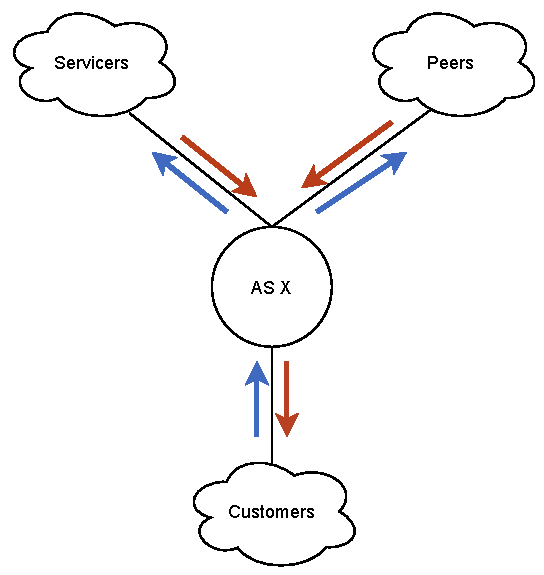
\includegraphics[scale=0.75]{images/BGP/ASKnowledgeDistribution.pdf}
	\caption{Distribution schema for the \acp{AS}, the row colours distinguish
	different flows, $AS\_X$ is a customer of the servicer set, a peer with the
	peers set and servicer for the customers set}
    \label{fig:AS_flow}
\end{figure}


As shown by the flows with a different colour in \Cref{fig:AS_flow} a single
\ac{AS} will share information considering the receiving link.
If something comes from one of its customers it will share the knowledge with
every other link that it has, even other customers (always respecting the output policies).
If a route has come from its provider or a peer then it will be only shared with
its own customers.
Those policies are commonly called \q{valley-free} and are dictated by convenience,
an \ac{AS} has all the advantages when
other \acp{AS} decide to use it to reach a specific destination.
For this reason is convenient for an \ac{AS} that everyone knows about its clients'
networks, and, on the opposite side, that its clients know only the route
through it to reach other networks.

This behaviour can be modelled with a variant of the \ac{SSP} algebra described
in \cite{daggitt2018rate}.
This is the same algebra that will be used in \Cref{cha:des} to describe the links
relationships.

%\begin{itemize}
%    \item BGP de facto standard on the internet
%    \item What is an AS
%    \item interconnection between ASes
%\end{itemize}

\section{The protocol in details}
\label{sec:bgp_intro}

Once a \ac{BGP} node has established a connection with another peer it will
start to exchange routes with that neighbour, always respecting the policies.
Its important to underline that, a \ac{BGP} speaker only shares its best routes
and in this protocol the best decision is dictated by the policies, and
then other possibilities would be evaluated (number of hops, bandwidth etc).
For this reason the best path decided by a node could differ from the actual
best path from a topological point of view.

Every \ac{BGP} node has a \ac{RIB} as data structure to keep the information
about the received routes, the alternative routes and what should be exported.
The \ac{RIB} is divided into \num{3} sections.
\begin{itemize}
	\item \textbf{\textit{ADJ-RIB\_in}:} This \ac{RIB} contains all the routes
		that have been received by other \ac{AS} in order to be evaluated;
	\item \textbf{\textit{LOC-RIB}:} This \ac{RIB} contains all the best routes
		that have been chosen from the \textit{ADJ-RIB\_in} from the node;
	\item \textbf{\textit{ADJ-RIB\_out}:} There is an output \ac{RIB} for every
		neighbour of the node, it contains the route that should be advertised
		to the specific node.
\end{itemize}

One of the most important parts of \ac{BGP} is its decision process, that would
be applied to discern between the routes in the \textit{ADJ-RIB\_in} in order
to update the \textit{LOC-RIB} and, if necessary also the \textit{ADJ-RIB\_out}.
The decision process is composed of three parts:
\begin{itemize}
	\item[1] Calculation of the preference: This function is called every time
		there are new reachability information that needs to be evaluated, it
		will assign/update the preference value at every route in the
		\textit{ADJ-RIB\_in} using policy filters pre-configured. If a route
		doesn't respect the policy filters it will be then marked as ineligible,
		otherwise, a \textit{PREF\_VALUE} will be calculated and assigned to the
		route;
	\item[2] Route selection: This function is called at the end of the first
		phase, it collects all the eligible routes and evaluates them removing
		routes that would create loops or that create conflicting situations.
		The evaluated routes are then ordered by the \textit{PREF\_VALUE} and
		then the best route will be then installed in the \textit{LOC-RIB}.
		In case of ties, there is an algorithm that can be used to break them;
	\item[3] Route dissemination: This function can be called in different
		situations, it will use the information in the \textit{LOC-RIB} to
		populate every \textit{ADJ-RIB\_out}, according to configuration
		policy.
\end{itemize}
The decision process is also responsible for the route aggregation and information
reduction.
At the end of the third phase, the \ac{BGP} speaker will execute the
\textit{Update-send} process, that is responsible for the effective dissemination.

There are multiple types of packets that can be sent by a \ac{BGP} speaker, but
I will focus only on the \ac{ADV} packets.
The \ac{ADV} packets are responsible for the dissemination of the information
to other nodes that will analyze and use the attribute inside the message
to assign a preference value to the route.
In particular, there are two sections of the \ac{ADV} messages that will
contain additive information and subtractive information.
Is possible to distinguish \ac{ADV} messages using the type of information that are
transmitting:
\begin{itemize}
	\item \textbf{\textit{UPDATE}:} This type of messages represents the distribution
		of new reachability information, a new best route to a destination will be
		shared through an update message;
	\item \textbf{\textit{WITHDRAW}:} This type of messages is distributed when
		a node want to share that it doesn't know how to reach
		a destination anymore.
\end{itemize}
Inside those packets, there are different attributes that permit to transfer
information about the route (advertised or withdrawn).
There is an attribute that describes the address that the route represents,
another one that contains the path that will be used to reach the
destination, the next-hop used, etc.
During the years multiple new \acp{RFC} have introduced, modified, updated and removed
attributes that can be found inside an advertisement message.
Not all the attributes are mandatory for \ac{BGP} nodes, in fact, for a node
is possible to receive a route with an attribute that it is not able to interpret
but (if configured to do so) it will share the route with also the unknown
attributes.

Is important to remember that all those information are useful for the policy
filters that every node can have, for example, some nodes would automatically discard
any route that contains a specific \ac{AS} in the received path.

The \textit{Update-send} process is responsible for the distribution of the
messages that are stored in the \textit{ADJ-RIB\_out}.
It executes again some checks on the \ac{RIB}, removing unfeasible routes
and removing routes that have already been advertised to the pear.
It also has to respect a temporal constraint, introduced in \cite{rfc4271},
a \ac{BGP} speaker can't send to the same neighbour routes for the same destination
more often than the \ac{MRAI} value.
\ac{MRAI} act as a timer whose goal is to avoid continuous update storm caused
by decision changes in some peers in the network.

Another property that can be found in \ac{BGP} nodes, that affects the messages
transmitted, is the \ac{IW}.
This property permits to reduce the number of messages that are distributed.
Without this option when a \ac{BGP} node discovers a new best path to reach
a destination should send a withdraw followed by an update to its neighbourhood.
Thanks to this option is sufficient to send just the update, the other nodes
will learn that the best path is changed simply looking to the previous
alternative and comparing them.

%\begin{itemize}
%    \item High level of BGP
%    \item BGP messages
%    \item BGP Update messages
%    \item BGP policies
%	\item two type of BGP noise, the one caused by BGP itself and the one
%		caused by flapping interfaces
%\end{itemize}

%\section{BGP Wedgies}
%\label{sec:bgp_wedgies}
%
%\begin{itemize}
%    \item What are wedgies?
%    \item why are them important?
%    \item which situations them occur?
%\end{itemize}

\section{BGP inherent noise vs external noise}
\label{sec:bgp_noise}

With the term \textit{BGP Noise}, I define a particular behaviour
of \ac{BGP}.
It underlines a situation where the nodes are distributing routes
that would be retrieved a few moments later.
Non-optimal messages are shared while nodes don't have a compleate knowledge
to take the best possible solution, producing multiple \ac{ADV} storms.
This behaviour is defined as noise because of the tendency of \ac{BGP} to act
as an echo-chamber amplifying this distribution of incorrect information.
%All those wrong messages are going to disturb the convergence of the protocol.
In fact, a \ac{BGP} node that receives an update from a neighbour will probably
redistribute the route to multiple neighbours, peers and servicer.
Given the hierarchical topology of the Internet, this behaviour grows
exponentially while the information reaches the centre of the network.

There are basically two sources of noise in \ac{BGP}, the inherent noise of
the protocol and the noise caused by external sources.
Those two types of noise are triggered by different causes and are
not discernible from one another.
Because, both the noise situations are characterized by an intense distribution
of messages and there are no other distinguishing features.

The first one is caused by the protocol itself when it tries to converge
on new knowledge.
The sharing of new routes can cause new \ac{ADV} that can then trigger the
\textit{Path Exploration} problem.
This is a noise caused by the protocol itself that distributes \ac{ADV} for
new paths that will change until the best possible path is taken into consideration.

One \ac{BGP} parameter tries to limit this noise acting as a message cache with
a compression system.
This parameter is \ac{MRAI} and it permits to avoid sending a message for every
new one received using a timer.
Only the best decision after that delay will be shared.

The second type of noise is caused by a source outside the protocol.
A miss-configuration or a faulty interface can cause the transmission of not necessary messages.
For example, the withdraw and the advertisement of a route at a continuous interval.
This type of behaviour will cause continuous storms of messages and the triggering
of the first noise type.
Also, the transmission of a withdraw followed by an announcement is considered
a \q{flap}.

\ac{BGP} introduce a parameter with the \ac{RFC} \num{2439} \cite{rfc2439} that
is called \ac{RFD} to overcome this behaviour.
This parameter increases a value every time a flap or a route change is detected,
when this value passes a predefined threshold the route will be suppressed.
This value will always decay using an exponential decay function, even if it
doesn't overpass the threshold.
The decay function is calculated defining the time that the function should take
to half the value, by default \SI{15}{\minute}.
Once the route has been suppressed the \ac{BGP} speaker must wait enough time
that the value goes below another indicator before sharing it again.

Those two parameters are clearly connected one another from the fact that
one triggers the other and vice versa, is possible to create a particular topology
that has different performances based on the values assigned to those
parameters.
Think about two clique networks interconnected by only one node, that
node will act as a bottleneck, probably its \ac{RFD} threshold would be easily
overpassed and then it depends on its decay function before it can share
again the prefix to the second clique triggering \ac{MRAI} on those nodes that
will experience the path exploration problem.

%\fxfatal{I think that the graphs in Fig 2 and Fig 3 of Fabrikant et al. in
%\cite{fabrikant2011there} will easily trigger both \ac{MRAI} and \ac{RFD}}

\section{BGP MRAI, designed to reduce inherent noise}
\label{sec:bgp_mrai}

\ac{MRAI} is one of the parameters that mostly affect the convergence of \ac{BGP}.
A high value of it could unnecessarily delay the transmission of messages, but,
in the opposite case, a value too small can provoke a lot of messages, one for
every decision change of the node.
The main function of it is to reduce the intrinsic noise of \ac{BGP} compressing
the set of messages received.
There are a lot of studies about it, and it has already been shown that
the number of messages and the convergence time can depend on it~\cite{griffin2001experimental}.
Also, it has been already proven by Fabrikant, Rexford et al.~\cite{fabrikant2011there}
that an incorrect configuration of it could lead to tremendous consequences.

\ac{MRAI} has been introduced in the \num{4}th version of \ac{BGP}~\cite{rfc4271} and
it is nowadays a mandatory mechanism for every \ac{BGP} node, otherwise the load
in terms of messages to process and decision changes would be incalculable.
Its main purpose, as anticipated in \Cref{sec:bgp_noise}, is to prevent or
at least mitigate the noise created by \ac{BGP} itself.

The most important component of \ac{MRAI} is a timer that controls how much time must pass
between one \ac{ADV} and the following one.
The timer is peer-based, for each interconnection an \ac{AS} could have a different
\ac{MRAI}, but it acts for every destination in parallel, this means that there
is a different timer for each destination that a node would share for every
\ac{BGP} relations that it has.
The idea behind it is that, in the period of time between one \ac{ADV} and the
following one the \ac{BGP} node will be able to receive other possible routes.
The enriched set of possibilities would give to the speaker the ability to take
a decision closer to the absolute best.
\ac{MRAI} has the property to compress the input messages sequence in order to have
an output message sequence with a smaller number of \ac{ADV}.

The behaviour of a \ac{BGP} node with \ac{MRAI} is defined as follow for every
change in the \textit{ADJ-RIB\_out} of a neighbour caused by the
\textit{Update-send} process:
\begin{itemize}
	\item If there isn't an active \ac{MRAI} timer for the destination changed
		send the \ac{ADV} and set an \ac{MRAI} timer;
	\item If there is an active \ac{MRAI} timer for the destination then
		don't send anything;
	\item When the active \ac{MRAI} timer ends if there is still the necessity
		to send an \ac{ADV} then send it and set another \ac{MRAI} timer.
\end{itemize}

The second passage permits the route selection process to be executed multiple
times before the actual transmission of the decision.
That because \ac{MRAI} limits only the transmission and not the decision process.
The condition to the last passage is due to the fact that the compression some
times could lead to the not necessity to actually send a message.

The default value defined in the \ac{RFC} \num{4271} for \ac{MRAI} is equal to
\SI{30}{\second}.
But, \ac{MRAI} is a really controversial parameter, it has received multiple
revisions and studies.

In \num{2008}, thanks to different studies that take into consideration the
dimension of the topology and the latency~\cite{qiu2005optimal}, there has been
the proposal to reset its default value to \SI{5}{\second}~\cite{jakma2008revised}
In \num{2010}, a proposal \ac{RFC} of the \ac{IETF}~\cite{jakma2010revisions}
says that the default value would be left to the arbitrary choice of the operators and
that withdraw message could completely ignore it.
But, this freedom would damage the convergence and the number of messages distributed
as showed by Fabrikant et al.~\cite{fabrikant2011there}.

Is clear that \ac{MRAI} affect the network performances, but what affects \ac{MRAI}
and, by consequences, the performances?
Obviously, the choice itself of a different \ac{MRAI} strategy can have a huge
impact, as showed for example in~\cite{milani2019BGP}, where the centrality
has been used to obtain better results in the case of network faults.
But, giving the fact that, the main function of \ac{MRAI} is to compress the
input messages, also the sequence of messages receipt could be meaningful.
Giving that \ac{MRAI} is a link-based parameter also the number of links that
a node has could influence it and by consequences the position in the topology.
A well connected node will be more likely to receive multiple paths and messages
than one with only one link.

\section{BGP RFD, designed to reduce external noise}
\label{sec:bgp_rfd}

\ac{RFD} is a parameter introduced in \ac{BGP} to overcome the problems caused
by exterior sources of noise.
Its main function is to avoid the computation overload provoked by fluctuating
routes with continuous message storms.
It has been introduced with the \ac{RFC} \num{2439} in \num{1998}~\cite{rfc2439}.
Also, \ac{RFD} is a controversial parameter, it has been studied and evaluated again
different times, but, recent studies showed that the majority of the operators
still use deprecated values from \num{2001}~\cite{gray2020bgp}.
Furthermore, other studies show that the majority of the \ac{ADV} that travels
through the Internet are generated by a restricted set of \acp{AS}, but \ac{RFD}
seems to be too much restrictive and affect the majority of the \acp{AS} traffic~\cite{pelsser2011route}.

\ac{RFD} will use a single value, called \textit{figure of merit}, to evaluate
the actual situation of a route, while this value evolves the \ac{RFD} algorithm
will make a decision on what to do.
The evolution of the \textit{figure of merit} is dictated by the messages received,
with fluctuations it will grow, while, over time, it will use a quadratic decay
function to decrease.
Fluctuations, or flaps, are represented by the reception of the withdraw and
the announcement of a route, a path change is also considered a flap, even
if thanks to \ac{IW} is limited to just one \ac{ADV}.

There are other parameters that are part of this \ac{BGP} component, the more
important are presented in \Cref{tbl:rfd_defaults}.

\begin{table}[ht]
	\begin{center}
	\begin{tabular}{ || m{5cm} | m{4cm} | m{4cm} || }
	\hline
			Parameter & Cisco default values & Juniper default values\\
	\hline \hline
			withdrawal penalty & 1.0 & 1.0 \\
	\hline
			re-advertisement penalty & 0.0 & 1.0 \\
	\hline
			attribute change penalty & 0.5 & 0.5 \\
	\hline
			suppress threshold & 2.0 & 3.0\\
	\hline
			half-life (min) & 15 (900s) & 15 (900s)\\
	\hline
			Reuse Threshold & 0.75 & 0.75 \\
	\hline
			Max Suppress Time (min.) & 60 (3600s) & 60 (3600s)\\
	\hline
	\end{tabular}
\end{center}

		\caption{\ac{RFD} parameters}
	\label{tbl:rfd_defaults}
\end{table}

Other than the name of the parameters, in \Cref{tbl:rfd_defaults} is showed also
the default value decided by Cisco and Juniper.
The \ac{RFC} \num{2439}~\cite{rfc2439} gives some guidelines on how to set those
values but the actual choice is left to the discretion of implementors.
The first three parameters, \textit{Withdraw, re-advertisement, attribute change}
represent the penalty applied to the \textit{figure of merit} when the homonym event
happen.
The \textit{suppression threshold} represents the level at which the \ac{BGP} node will
suppress the route and don't advertise it until the figure of merit goes
below the \textit{reuse threshold}.
The decay of the \textit{figure of merit} follows a quadratic decay function
which rate is calculated using the \textit{Half-life} parameter.
The \textit{Max Suppress Time} will override all these parameters because, as
defined in the original \ac{RFC}, a route cannot be suppressed for more than
that time, it doesn't matter the figure of merit accumulated by this route.

An example of the figure of merit evolution could be seen in \Cref{fig:figure_of_merit},
This image has been taken from \cite{gray2020bgp}.

\begin{figure}[ht]
    \centering
    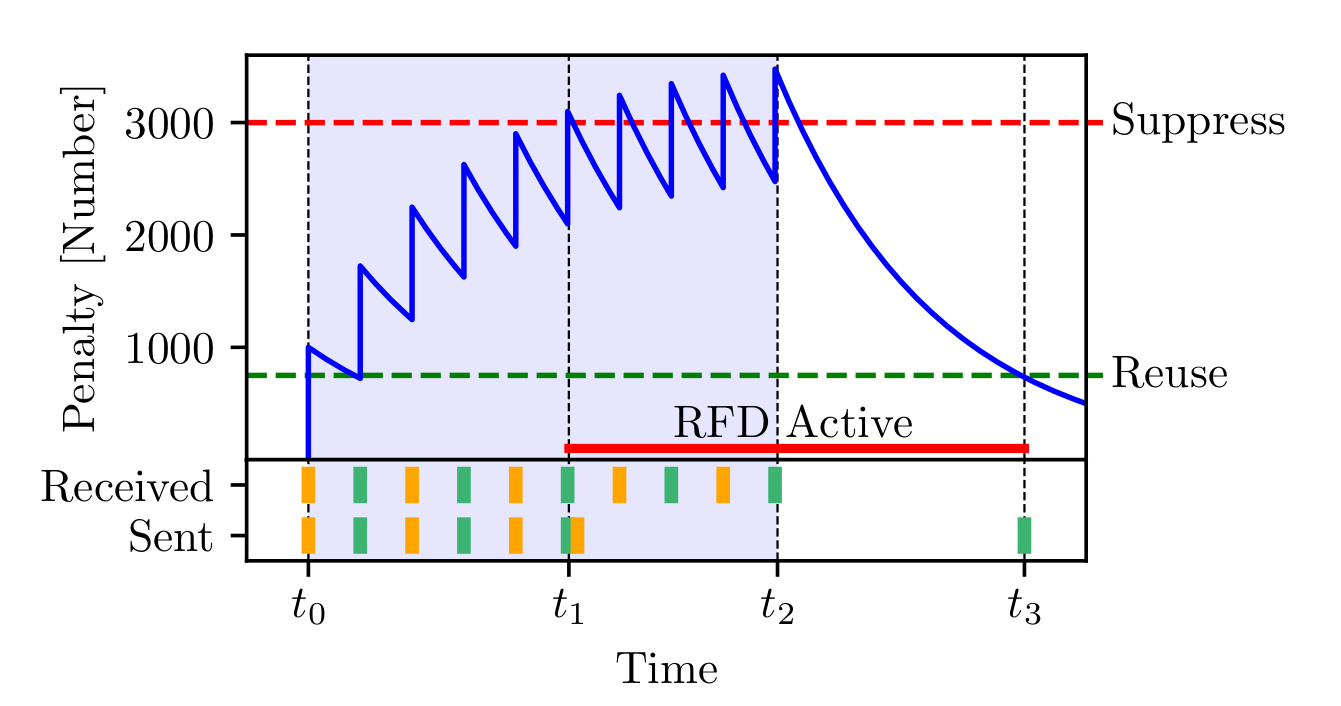
\includegraphics[scale=0.22]{images/RFD/evolution.png}
	\caption{Example of evolution of the \ac{RFD} \textit{figure of merit} taken
	from \cite{gray2020bgp}, yellow messages represent withdraws and green ones
	are advertisement, the dashed lines are the suppression and reuse threshold}
    \label{fig:figure_of_merit}
\end{figure}

\Cref{fig:figure_of_merit} shows a hypothetic evolution of the \ac{RFD} filter,
it doesn't rely on the default value of the Cisco or Juniper implementation.
Is possible to see, in the lower part of the plot, the messages received by the
\ac{BGP} speaker, yellow one represent withdraws while the green are announcements.
Is possible to see that the penalty value grows at each flap and as soon it reaches
the suppression threshold the route will not be advertised to any neighbour.
While after the decay has reached the reuse level is possible to advertise the
route again.

Is possible to see that \ac{RFD} doesn't make any difference on its own on what
is causing the flaps, it simply constant reacts to the evolution of the network.
Is not even possible to determine where is located the flap, if the source
is flapping heavily for some reasons or there is an \ac{AS} in the middle of the
path that is malfunctioning.

\ac{RFD} has a troubled history, maybe even more than \ac{MRAI}.
In \num{2006}, thanks to the publication of \cite{mao2002route}, the \ac{RIPE}
recommends to disable it\cite{smith2006ripe}.
A few years later, after the publication of the article from Pelsser et al.~\cite{pelsser2011route}
\ac{RIPE} and \ac{IETF} shares that now \ac{RFD} should be used with the updated
parameters \cite{bush2013ripe,rfc7196}.
Unfortunately, the study from Gray et al. \cite{gray2020bgp} in \num{2020} shows
that the majority of the \ac{AS} uses \ac{RFD} with outdated parameters
from the \ac{RFC} \num{2439}.

\ac{RFD} can influence the network convergence time, and this behaviour is
mostly impacted by the threshold and the decay function applied to the figure
of merit.
A more permissive threshold could be helpful in situations where the flaps are
caused by transitory behaviour.
I will study and analyze the impact of the threshold in \Cref{cha:bgp_rfd}.

%\begin{itemize}
%    \item What is RFD?
%	\item Remember that RFD purpose is to avoid the noise produced
%		by route flapping
%	\item RFD cant distinguish the noise, is to restrictive, R bush point to
%		avoid the use of RFD for the first noise increasing the threshold.
%    \item Why is used RFD?
%    \item Evolution of RFD?
%    \item RFD Today
%\end{itemize}

\section{Topologies}
\label{sec:topologies}

\ac{BGP} has been designed to hide information, it is possible to remove attributes
from packets or aggregate them.
For this reason, a \ac{BGP} node must overlap the received information with the
policies.
Topological information can be overwritten in order to respect the policies and
the further nodes in the network will never know the difference.

Is important to remember that the actual topology of the Internet depends on the
level of abstraction required.
Considering the graph of the relationships within the \acp{AS} is not
possible to assume that this also represents the geographical graph.
In fact, one \ac{AS} can have multiple connections with another \ac{AS}
that are distributed along different geographical points.
Is also possible to have a connection through a tunnel that will permit to have
a link that physically passes over other devices.
Is possible to see an example of this distinction in \Cref{fig:astopology_vs_internet}

\begin{figure}[ht]
     \centering
     \begin{subfigure}[b]{0.45\textwidth}
         \centering
         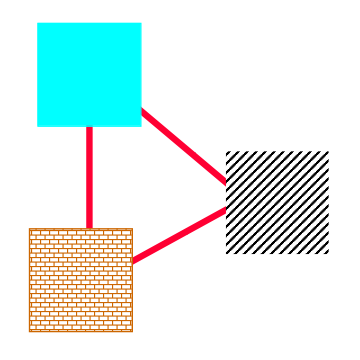
\includegraphics[width=\textwidth]{images/BGP/ASTopology.png}
		 \caption{\ac{AS} Graph}
         \label{fig:as_graph}
     \end{subfigure}
     \hfill
     \begin{subfigure}[b]{0.45\textwidth}
         \centering
         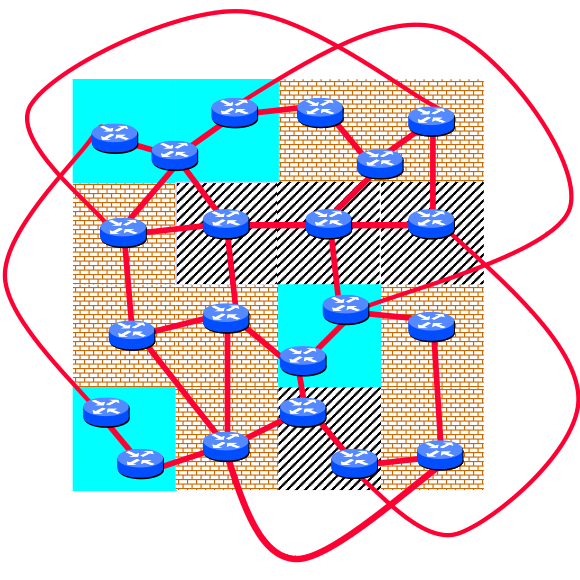
\includegraphics[width=\textwidth]{images/BGP/InternetTopology.png}
		 \caption{Actual geographical topology}
         \label{fig:actual_topology}
     \end{subfigure}
		\caption{Differences between two levels of detail on the Internet graph.
		 From SIGCOMM 2001 BGP tutorial by Timothy G. Griffin}
        \label{fig:astopology_vs_internet}
\end{figure}

In this thesis I will consider only the first case, all my topologies are composed of
the connections between the \acp{AS} without considering the actual physical layer
where these interconnections reside.

I will then use three different topologies to show particular situations or
behaviours of the network with certain events.
\begin{itemize}
	\item \textbf{\textit{Clique topology}:} This topology represent the higher
		level of the internet, in fact, all the Tier one nodes are interconnected
		in a clique network;
	\item \textbf{\textit{Fabrikant topology}:} This is a particular topology
		because it represents a special case that can be present on the internet,
		and also is possible to show that special configurations of this topology
		can lead to problematic situations;
	\item \textbf{\textit{Internet-like topology}:} This kind of topologies
		have the goal to resemble the real internet using statistical information
		about it.
\end{itemize}

I choose the clique topology because it is one of the possibly worst
case scenario for a \ac{BGP} network, accordingly with~\cite{labovitz2000delayed}.
A clique graph could be composed by $n$ nodes, and every node has
$n-1$ edges towards every other node.
An example of clique topology can be sawed in \cref{fig:clique_topology}, I added
two nodes to the network, outside the clique, in order to be able to have an
input and an output point.

The Fabrikant topology is inspired by~\cite{fabrikant2011there}, where
a similar chain network is used to show, in a theoretical way, how an uncontrolled
\ac{MRAI} setting could lead to explosive situations.
This topology will be used for the same purpose in this thesis, an example
of it is showed in \Cref{fig:fabrikant_topology}.
The explosion is caused by the \textit{Path exploration} problem, at a certain
point the node \num{2} would change idea on which path to follow to reach $d$
and all nodes will go through a transition state where they will
share their backup paths.

\begin{figure}[ht]
     \centering
     \begin{subfigure}[b]{0.45\textwidth}
         \centering
		 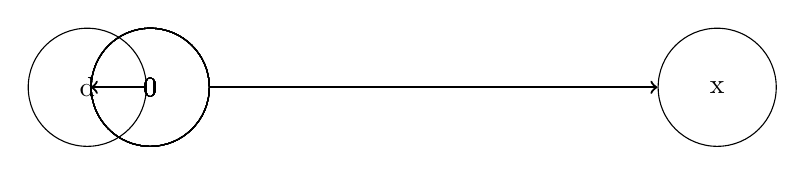
\begin{tikzpicture}[scale=0.2, every node/.style={draw=black,circle,inner sep=0pt}]
    \node [minimum size=1.5cm] (d) at (0,0) {d}; 
    \node [minimum size=1.5cm] (x) at (40,0) {x};                                    
    \node [minimum size=1.5cm] (0) at (4,0) {0};                                    
    \node [minimum size=1.5cm] (0) at (4,0) {0};                                    
    \node [minimum size=1.5cm] (0) at (4,0) {0};                                    
    \node [minimum size=1.5cm] (0) at (4,0) {0};                                    
    \node [minimum size=1.5cm] (0) at (4,0) {0};                                    
    \node [minimum size=1.5cm] (0) at (4,0) {0};                                    
    \node [minimum size=1.5cm] (0) at (4,0) {0};                                    
    \node [minimum size=1.5cm] (0) at (4,0) {0};                                    
    \node [minimum size=1.5cm] (0) at (4,0) {0};                                    
    \node [minimum size=1.5cm] (0) at (4,0) {0};                                    
    \draw [thick, ->] (d) -- (0);                                 
    \draw [thick, ->] (0) -- (x);                                 
\end{tikzpicture}                                                       
		 \caption{Clique graph example}
    	 \label{fig:clique_topology}
     \end{subfigure}
     \hfill
     \begin{subfigure}[b]{0.45\textwidth}
         \centering
         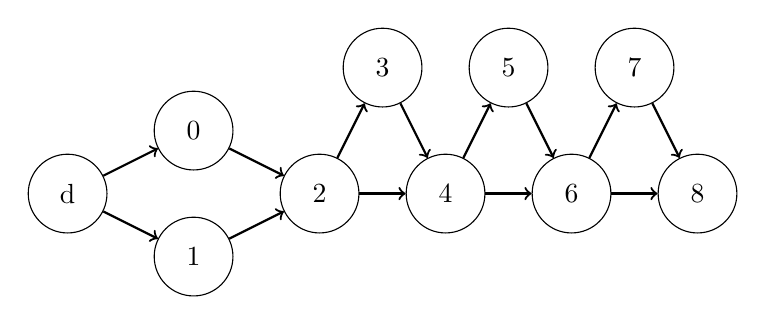
\begin{tikzpicture}[scale=0.2, every node/.style={draw=black,circle,inner sep=0pt}]
    \node [minimum size=1cm] (d) at (0,0) {d}; 
    \node [minimum size=1cm] (0) at (8,4) {0}; 
    \node [minimum size=1cm] (1) at (8,-4) {1}; 
    \node [minimum size=1cm] (2) at (16,0) {2}; 
    \node [minimum size=1cm] (3) at (20,8) {3}; 
    \node [minimum size=1cm] (4) at (24,0) {4}; 
    \node [minimum size=1cm] (5) at (28,8) {5}; 
    \node [minimum size=1cm] (6) at (32,0) {6}; 
    \node [minimum size=1cm] (7) at (36,8) {7}; 
    \node [minimum size=1cm] (8) at (40,0) {8}; 
    \draw [thick, ->] (d) -- (0);
    \draw [thick, ->] (d) -- (1);
    \draw [thick, ->] (0) -- (2);
    \draw [thick, ->] (1) -- (2);
    \draw [thick, ->] (2) -- (3);
    \draw [thick, ->] (2) -- (4);
    \draw [thick, ->] (3) -- (4);
    \draw [thick, ->] (4) -- (5);
    \draw [thick, ->] (4) -- (6);
    \draw [thick, ->] (5) -- (6);
    \draw [thick, ->] (6) -- (7);
    \draw [thick, ->] (6) -- (8);
    \draw [thick, ->] (7) -- (8);
\end{tikzpicture}                                                       


		 \caption{Fabrikant chain graph example}
		 \label{fig:fabrikant_topology}
     \end{subfigure}
		\caption{Simple topologies used in the thesis}
        \label{fig:clique_and_fabrikant}
\end{figure}

The last type of topology used points to resemble the properties of the actual
Internet graph.
It uses the property studied and described by Elmokashfi et al. in \cite{elmokashfi2010scalability}.
An example with few nodes is available in \cref{fig:internet_like_topology}.
The internet graph is actually a hierarchical graph clearly separated in multiple
levels by the type and properties of the nodes.

\begin{figure}[ht]
     \centering
     \begin{subfigure}[b]{0.8\textwidth}
		 \centering
		 \begin{tikzpicture}[scale=0.2, every node/.style={draw=black,circle,inner sep=0pt}]
		\node [draw=white] (l) at (-3,0) {\textbf{Legend:}};
		\node [minimum size=.5cm,fill=red] (t) at (4,0);
		\node [draw=white] (tl) at (9,0) {Tier one};
		\node [minimum size=.5cm,fill=orange] (m) at (16,0);
		\node [draw=white] (ml) at (22,0) {Mid-Level};
		\node [minimum size=.5cm,fill=yellow] (cp) at (30,0);
		\node [draw=white] (ml) at (39,0) {Content provider};
		\node [minimum size=.5cm,fill=violet] (c) at (50,0);
		\node [draw=white] (ml) at (56,0) {Customer};
\end{tikzpicture}

     \end{subfigure}
     \begin{subfigure}[b]{0.49\textwidth}
         \centering
         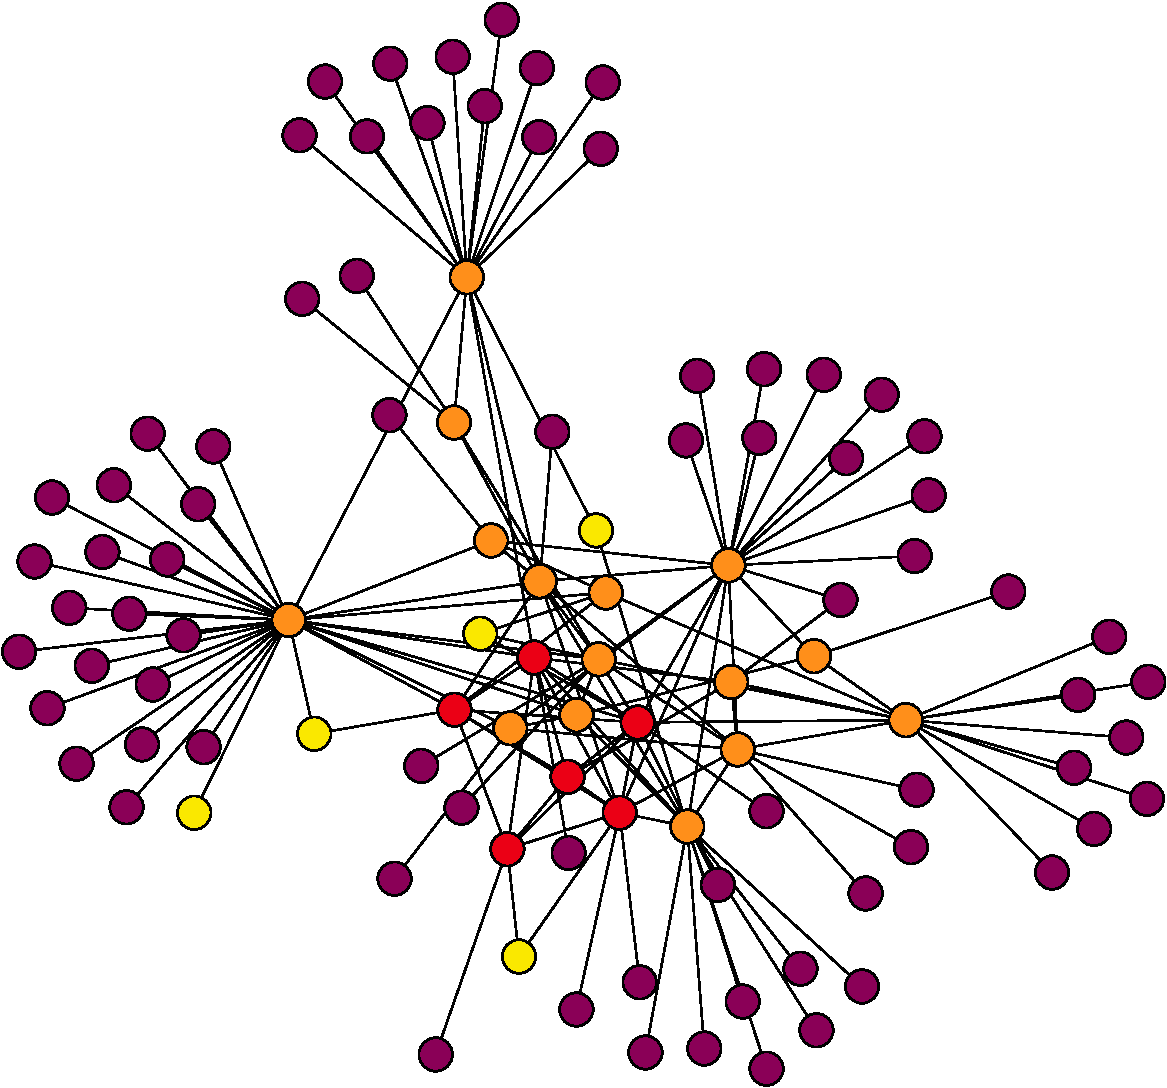
\includegraphics[width=\textwidth]{images/internet_graph/graph-100-colored.pdf}
		 \caption{Internet like graph with an \q{explosive} layout}
         \label{fig:internet_topology_explosive}
     \end{subfigure}
     \hfill
     \begin{subfigure}[b]{0.49\textwidth}
         \centering
         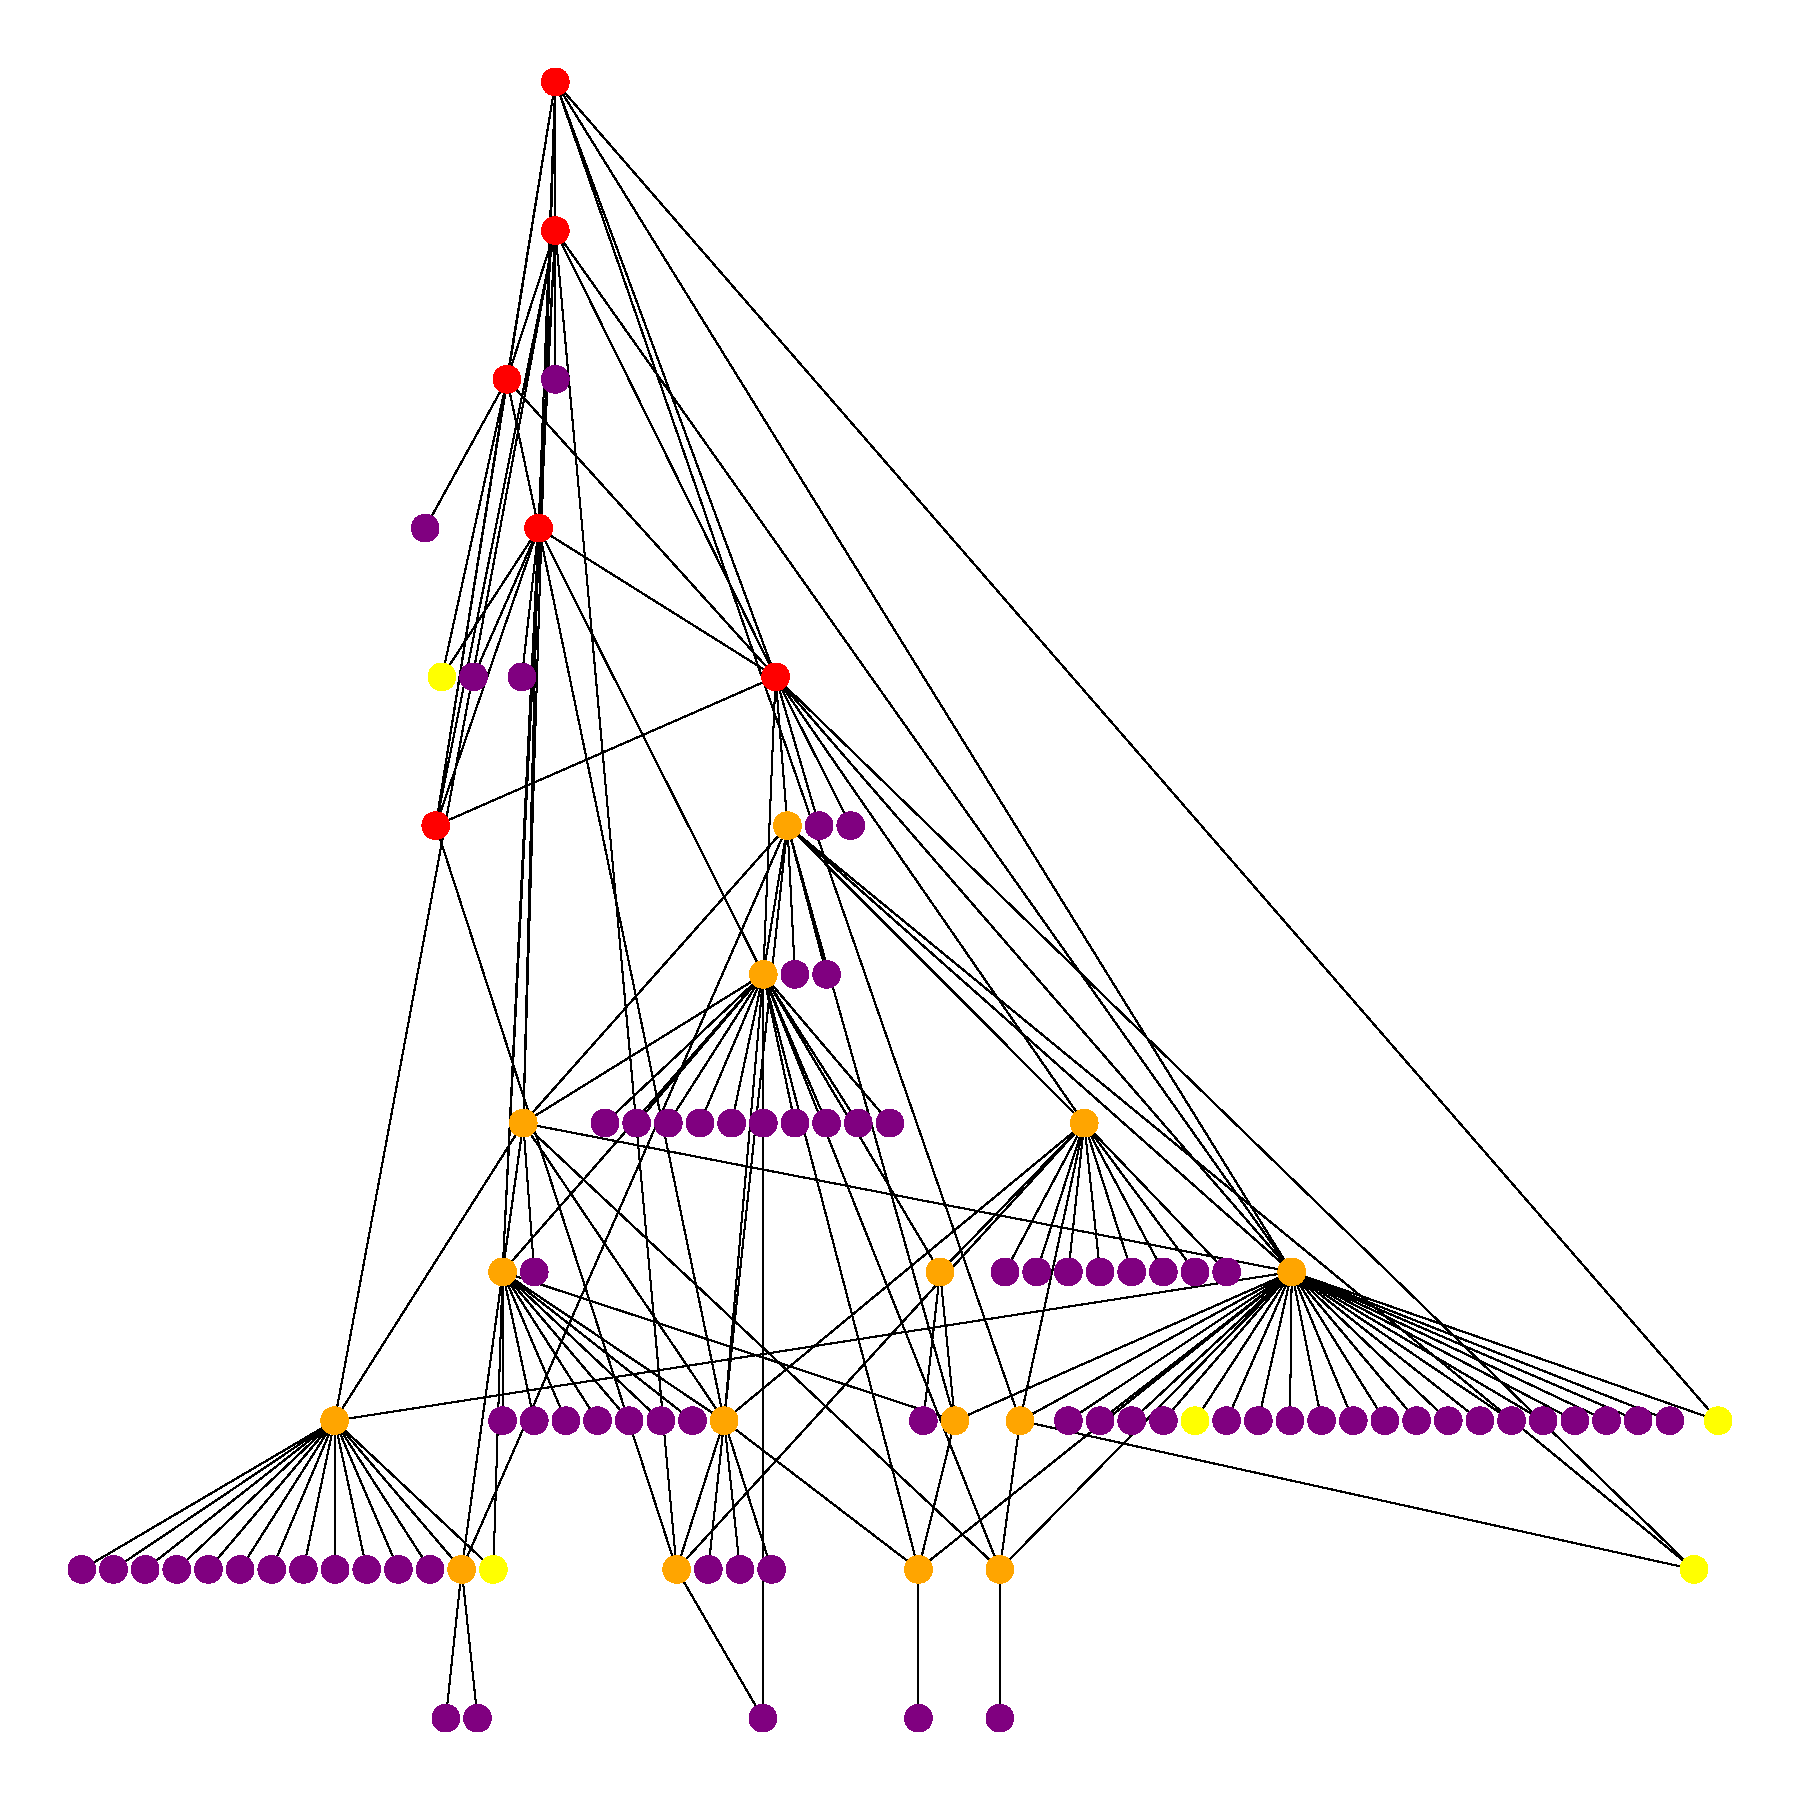
\includegraphics[width=\textwidth]{images/internet_graph/graph_dot.pdf}
		 \caption{\q{Hierarchical} Internet like graph}
         \label{fig:internet_topology_hierarchical}
     \end{subfigure}
        \caption{Internet like graph coloured to show the hierarchical structure,
		4 types of nodes}
		%\rlc{Aggiungi una legenda con i colori, puoi fare un'altro disegno e assiiungerlo sotto le topologie}
        \label{fig:internet_like_topology}
\end{figure}

    \chapter{Discrete Event Simulator}
\label{cha:des}

Experiments on \ac{BGP} are not applicable on the Internet, for this
reason different studies show their results using a simulate environment
\cite{griffin2001experimental} \fxfatal{Insert other citations}.
The majority of the studies uses small graphs and each node 
of the graph simulate the behaviour of a \ac{BGP} speaker.
Each node represent also a single \ac{AS} and the \ac{BGP} speaker is it's own
exterior router, for simplicity, reduced to one speaker that handles all the
connections. 
 
For this reason, I decided to use and expand a \ac{DES} that permits to have
different grades of freedom, respecting on the other side all the properties
required for a reliable simulator environment.
I decided to use the \textit{Simpy}\footnote{\href{https://simpy.readthedocs.io/en/latest/index.html}{Simpy website}}
package to make the environment evolve. I decided for this package for the
extensive documentation and because it has been already used for different
studies, demonstrating its adaptability \cite{matloff2008introduction,dagkakis2013manpy}.

I developed the \ac{DES} as a highly modular environment.
\begin{figure}[h]                                                               
    \begin{center}                                                              
        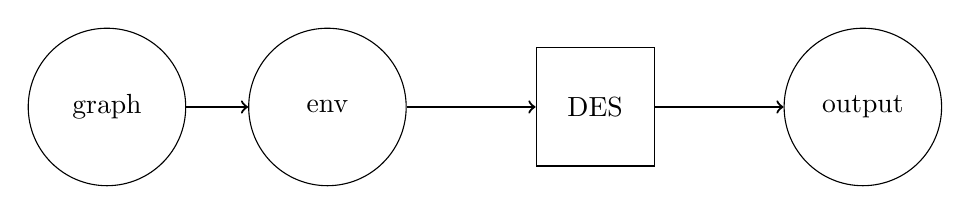
\begin{tikzpicture}[scale=0.2, every node/.style={draw=black,circle,inner sep=0pt}]
    \node [minimum size=2cm] (graph) at (0,0) {graph}; 
    \node [minimum size=2cm] (env) at (14,0) {env};                                    
    \node [rectangle, draw, minimum width=1.5cm,minimum height=1.5cm] (des) at (31,0) {DES};
    \node [minimum size=2cm] (output) at (48,0) {output};                                    
    \draw [thick, ->] (graph) to (env);                                  
    \draw [thick, ->] (env) -- (des);                                 
    \draw [thick, ->] (des) -- (output);                                 
\end{tikzpicture}                                                       

    \end{center}                                                                
    \caption{Discrete event simulator structure}                                
    \label{fig:des_structure}                                                   
\end{figure}

In \Cref{fig:des_structure} is possible to see the basic idea of the simulator.
The first component needed is a graph, represented by a \textit{graphml} file, 
this file is the descriptor of the network. 
it defines also all topological information and all the properties of every single node.
In Code \ref{lst:graph_example} is possible to see an example of a \textit{graphml} file,
it describes that node \num{0} contains a single destination and that the edge
between nodes \num{2} and \num{5} is controlled by the policy |2, 2, 2| that defines
a servicer-provider policy.
Policies are encoded using the convention described in \cite{daggitt2018rate}.

\lstcaptionname{Code}
\begin{lstlisting}[language=graphml, caption=Graph example, label=lst:graph_example]
 <node id="0">
      <data key="d0">10.0.0.0/24</data>
 </node>
 <edge source="2" target="5">                                                  
     <data key="d2">2, 2, 2</data>                                             
 </edge> 
\end{lstlisting}

The graph is then embedded in the environment file, this file is in \textit{JSON}
format and it describes how the environment is characterized, it gives the 
initial values for the \ac{RNG} so that each experiment is replicable and
other properties, like where the output should be saved, and, most importantly
how the experiment should be conducted.
There is two possible evolution of the environment:
\begin{itemize}
    \item \textbf{\textit{Continuous evolution}}: In this category all the nodes
    that contains at least a destination will continuously share and retrieve
    the destination accordingly with the distributions defined in the environment;
    \item \textbf{\textit{Signaling evolution}}: Is possible to define a precise
    signal that should be executed by the nodes that contain a destination, for 
    example, the signal \q{AWA} defines that there will be an announce followed by 
    a withdraw and another announce.
\end{itemize}

The \ac{DES} take as input this \textit{JSON} file where all the information
are described, it creates an object for each node in the graph file, with
each own characteristics.
After the initialization, all the nodes that contain a destination will schedule
the first advertisement of it to their neighbour.
The simulation run will terminate only if there are no more events scheduled or
if the maximum simulation time is reached.

The \ac{DES} will then produce a \textit{CSV} output, with all the events that 
can be analyzed to see the evolution of a specific node or to evaluate the
whole network.
 
\section{DES Environments}
\label{sec:des_environment}

Thanks to the environment codification in a \textit{JSON} file is possible to
define experiments with a high grade of freedom. 
Is possible to define multiple delays as probability functions vectors that
will provide multiple runs possibility. For example, if we have \num{5} different
possible seeds and \num{3} different delays, the total number of runs combinations
is \num{15}, as shown in Code \ref{lst:environment_example}.
is possible to run one of the possible combinations of parameters through the identifier
of the single run.

\lstcaptionname{Code}
\begin{lstlisting}[language=json, caption=Environment example, label=lst:environment_example]
"simulation" : {                                                              
    // seed(s) to initialize RNG                                      
    "seed" : [0, 1, 2, 3, 4], 
    ....
    // Multiple withdraw distributions
    "withdraw_dist": [{"distribution": "unif", "min": 5, "max": 10, "int": 0.1},
                      {"distribution": "unif", "min": 8, "max": 10, "int": 0.1},
                      {"distribution": "unif", "min": 2, "max": 3, "int": 0.1}],       
    ....
}
\end{lstlisting}

In the environment is possible to define also the processing time, this time is used
inside each \ac{BGP} node to emulate the processing of information or the evaluation
of a packet.
Though the \textit{delay} parameter is possible to define the default delay on the edges,
is important to remember that the links are FIFO so there is no reordering
of messages in the same link, there is also no messages lost.
That because it was out of the scope of this thesis to study the evolution
of the protocol with packet loss, but it could be future work.

\subsection{Clique environment}
\label{subsec:clique_env}

One of the special environment that I used in my experiments uses clique 
graphs of different dimensions, an example of the clique graph is given in
\Cref{fig:clique_topology}.

The only node that shares a destination is the node \q{\textit{d}}, the node
\num{0} will then spread the knowledge to the whole network, and the node 
\q{\textit{x}} will act as a black hole for all the possible paths
that the node \num{5} will share.

This topology is used to enforce the \textit{Path exploration} problem, it also
gives the possibility to study how \ac{BGP} parameters can influence the messages
distribution in stressful cases like the clique one.
I'm going also to study how the variation of those parameters from the standard
ones can impact the performances in this environment of high load.

\subsection{Fabrikant environment}
\label{subsec:fabrikant_env}

Another interesting chase to test the path exploration problem is the one
presented in \cite{fabrikant2011there}.
In that study, Fabrikant et al. presents how particular \ac{MRAI} setting could 
make the network converge with exponential behaviour because of the 
continuous decision change in terms of best paths from the nodes. 
I used the basic example of their study to investigate how the choice of \ac{MRAI}
is fundamental for the network convergence.
An example of the network used is presented in \Cref{fig:fabrikant_topology}.

The path exploration problem is caused by the delay on the \num{0}-\num{2}
edge. The node \num{2} will receive the destination through node \num{1}, after a small amount
of time the network will converge to the best path (without using the backup links).
But, after a while, node \num{2} will receive the network also through node \num{0}
and it will prefer this new path, provoking then the reconfiguration of all
the other nodes that will use the backup links for a while, announcing their 
new paths.
A wrong configuration of \ac{MRAI} can provoke the entire exploration of the 
possibility set.

This environment is also used to show how a \ac{BGP} \ac{FSM} would explode
in terms of possible states and edges producing an enormous ammount of possible
output signals from the same input.

\subsection{Internet-like environment}
\label{subsec:internet_like_env}

The last noteworthy environment is the one whose purpose is to simulate the Internet
behaviour.
This has been possible thanks to the study by Elmokashfi et al. \cite{elmokashfi2010scalability}
and the internet like graph generator present in Networkx \footnote{\href{https://networkx.org/documentation/stable/reference/generated/networkx.generators.internet_as_graphs.random_internet_as_graph.html\#networkx.generators.internet_as_graphs.random_internet_as_graph}{Networkx internet as graph generator}}
(a Python library famous for graph and network studies).
An example with a small set of nodes is presented in \Cref{fig:internet_like_topology}.

The different nodes are coloured accordingly with the node type represented.
The tier one nodes that generate the central clique are coloured in red and
is possible to notice in \Cref{fig:internet_topology_hierarchical} that they are
in the highest levels of the networks.
This environment has been used to study the behaviour of the network with 
topologies resembling the real internet.

In the next studies, I generally refer to this kind of topology with the 
terms \q{Internet-like}, and the dimension is never less than \num{1000} nodes,
otherwise is not possible to ensure all the Internet topological properties.

The goal of the experiments that use that kind of topologies is to study
the general network performances in terms of average convergence time and 
the number of messages transmitted.
This would help to see and study behaviours that are more typical in the actual
Internet.

    \chapter{The Protocol as a Finite State Machine}
\label{cha:bgp_fsm}

An \ac{FSM} could be useful for a lot of purposes, to debug the protocol, to 
understand what is happening, to analyze leeks.
It has been already done for a lot of protocols \fxfatal{insert citations}, but 
not for \ac{BGP}.

\fxfatal{Give more examples on what a protocol \ac{FSM} is useful for}

\section{BGP generalization}
\label{sec:bgp_generalization}

The main idea behind the \ac{BGP} \ac{FSM} is to represent the knowledge as
states and different set of messages as transitions.
The knowledge is represented by the actual routes that the node knows on how 
to reach a single destination.
Transitions encode the messages that a node has received to trigger the state change,
on the edges are also inserted the response messages that the node will transmit.
We can see an example of this transitions in \Cref{fig:fsm_example}

\begin{figure}[h]                                                               
    \begin{center}                                                              
        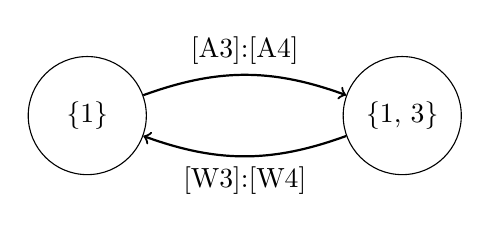
\begin{tikzpicture}[scale=0.2, state/.style={draw=black,circle,inner sep=0pt}]
	\node [state, minimum size=1.5cm] (s1) at (0,0) {\{1\}}; 
	\node [state, minimum size=1.5cm] (s2) at (20,0) {\{1, 3\}};
	%\draw[arrow](B1.west) to [out=190,in=170] node[above]{Flow: $\alpha$ } (S1.west);
	\draw [thick, ->] (s1) to[out=20, in=160] node[above]{[\q{A3}]:[\q{A4}]} (s2); 
	\draw [thick, ->] (s2) to[out=-160, in=-20] node[below]{[\q{W3}]:[\q{W4}]} (s1);
\end{tikzpicture}                        

    \end{center}                                                                
	\caption{Example of the \ac{BGP} \ac{FSM} state transition}
    \label{fig:fsm_example}                                                   
\end{figure}

In \Cref{fig:fsm_example} there are two states, both represent the knowledge of
the node, the first one represent the \ac{RIB} with just the route \num{1}, in
the second state the \ac{RIB} will contains both the routes \num{1} and \num{3}.
This transition si caused by the reception of the advertisement of the route 
\num{3} and will couse the transmission of an other advertisement.
The opposite transition is caused by the reception of the withdraw of the route
\num{4} with the consequent withdraw of the route \num{4}.

In \ac{BGP} messages transfer information about routes, there could be the advertisement
or the withdraw of the route.

Thanks to \ac{MRAI} the evaluation of multiple messages could be delayed and
provoke then the compression of them.
For this reason on the edges is possible to see multiple messages, for example 
\q{A1W1A1}, that will be compressed in \q{A1} and then evaluated.

The concept for a \ac{BGP} \ac{FSM} has been expanded from \cite{griffinFSM}.

%\begin{itemize}
%    \item BGP as an FSM main idea
%    \item signalling transmutation
%\end{itemize}

\section{BGP FSM experiments}
\label{sec:bgp_fsm_experiments}

The first experiments, about the translation of a single node evolution in a
\ac{FSM}, goal is to reproduce what has been shown in \cite{griffinFSM}.
The graph used for the study is presented in \cref{fig:griffin_fig_4}.

\begin{figure}[h]                                                               
    \begin{center}                                                              
        \begin{tikzpicture}[scale=0.2, every node/.style={draw=black,circle,inner sep=0pt}]
    \node [minimum size=1cm] (1) at (0,0) {1}; 
    \node [minimum size=1cm] (2) at (-8,-8) {2}; 
    \node [minimum size=1cm] (3) at (8,-8) {3}; 
    \node [minimum size=1cm] (4) at (0,-16) {4}; 
    \node [minimum size=1cm] (5) at (0,-24) {5}; 
	\draw [thick, ->] (0, 5) -- (1);
    \draw [thick, ->] (1) -- (2);
    \draw [thick, ->] (1) -- (3);
    \draw [thick, ->] (2) -- (4);
    \draw [thick, ->] (3) -- (4);
    \draw [thick, ->] (3) -- (5);
    \draw [thick, ->] (4) -- (5);
	\draw [thick, ->] (5) -- (0, -30)
\end{tikzpicture}                                                       


    \end{center}                                                                
	\caption{Graph from fig 4 of \cite{griffinFSM} used to study the \ac{FSM}
		of the nodes}                                
    \label{fig:griffin_fig_4}                                                   
\end{figure}

This topology, \Cref{fig:griffin_fig_4}, present an \ac{SPP} with five nodes \cite{griffin2002stable}. 
The \ac{SPP} model is used to eliminate much of the complexity of \ac{BGP}.
The arrows in the graph represent the flow of information, node \num{1} is the one
that will receive a new route to reach a hypothetical destination and it will 
spread this information through an \ac{ADV} to all it neighbours.
The translation to the \ac{CFSM} will use an enumeration to encode all the
paths that a single node will encounter, for example, the path \q{5 3 1} will
be converted in \textit{a3}, each path has its own identifier.
In case of withdraw the route will be encoded as \textit{w3}.

The properties of the environment for this experiment are listed in \Cref{tbl:fig_4_example}.

\begin{table}[h]
	\begin{center}
	\begin{tabular}{ || m{4cm}| m{8cm} || } 
	\hline
	Property & Value \\ 
	\hline \hline
	Seeds & $[1, 50]$ \\ 
	\hline
	Signaling & \q{AW} \\
	\hline
	Withdraws delay & Uniform distribution between \SI{20}{\second} and \SI{30}{\second} \\ 
	\hline
	Announcement delay & Uniform distribution between \SI{20}{\second} and \SI{30}{\second} \\ 
	\hline
	MRAI & \SI{0}{\second} for every link \\
	\hline
	Link delay & Uniform distribution between \SI{0.001}{\second} adn \SI{1}{\second}, uniform distribution between \SI{0.012}{\second} and \SI{3}{\second} \\
	\hline
	\end{tabular}
\end{center}

	\caption{FSM example environment properties}
	\label{tbl:fig_4_example}
\end{table}

The total number of runs generated by this environment is \num{100}.

\fxfatal{this paragraph is cumbersome}
The two nodes of more interest are node \num{4} and node \num{4}.
The first one can receive multiple combinations of messages from node \num{2} and
\num{3}, for sure there will be two announcements and two withdraws because node
1 has to respect a predefined signaling. but, those messages could be reordered
in different ways, and, for each sequence of them we can encounter a different
sequence of output messages through node \num{5}.
Giving that the routes from node \num{2} and \num{3} will have respectively as 
ID \num{2}, \num{3} the table \Cref{tbl:fig_4_node4_possible_inputs}
All possible inputs of node \num{4} are the shuffle of all possible
outputs of nodes \num{2} and \num{3} preserving the local order.

\begin{table}[h]
	\begin{center}
	\begin{tabular}{ || m{3cm}| m{3cm} || }
	\hline
	Input signal & Output signal\\
	\hline \hline
	$a2a3w2w3$ & $a4a5w4$ \\
	$a2a3w3w2$ & $a4w4$ \\
	$a3a2w2w3$ & $a5a4a5w5$ \\
	$a3a2w3w2$ & $a5a4w4$ \\
	$a2w2a3w3$ & $a4w4a5w5$ \\
	$a3w3a2w2$ & $a5w5a4w4$ \\
	\hline
	\end{tabular}
\end{center}


	\caption{Node 4 different possible inputs and output}
	\label{tbl:fig_4_node4_possible_inputs}
\end{table}

The node \num{5} will receive all the possible outputs from node \num{3} and 
\num{4} increasing the number of possible signals from \num{6} of node \num{4}
up to \num{71} but some of them produce the same output signal, so we have in 
total \num{52} unique output signals from node \num{5}.

From the \num{100} total runs we can generate the \ac{CFSM} of node \num{4} and
node \num{5}, in order to be able to study how the nodes reacts to different
input signals.
The two \ac{CFSM} are presented in \Cref{fig:fsm_griffin_fig4}.

\fxfatal{Remove message table from \Cref{fig:fsm_griffin_fig4}?}
\begin{figure}[h]
     \centering
     \begin{subfigure}[b]{0.45\textwidth}
         \centering
         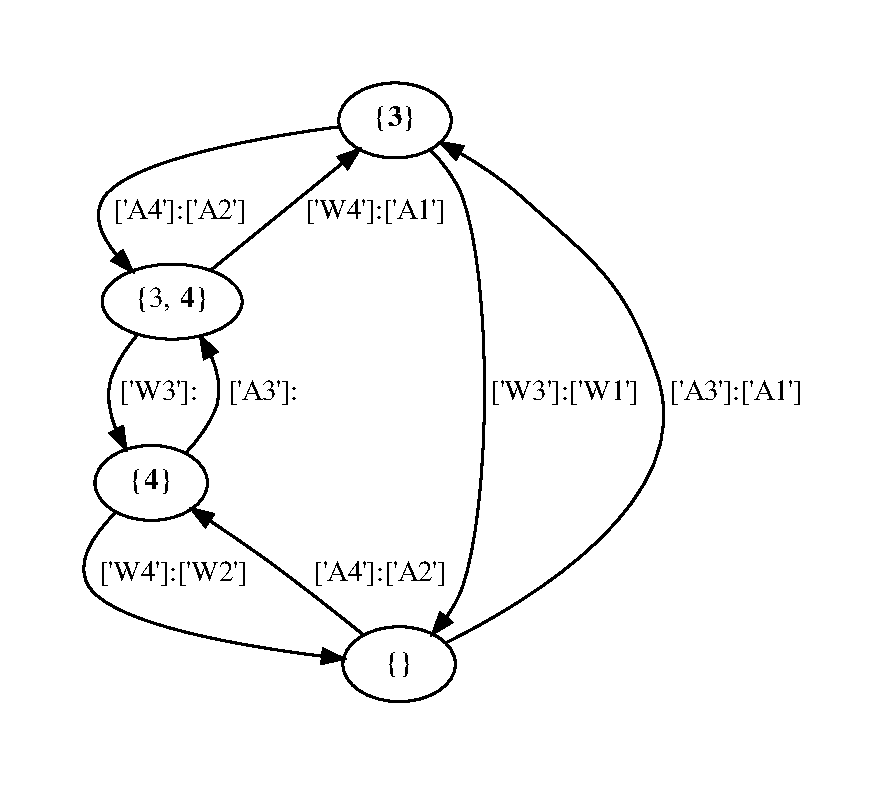
\includegraphics[width=\textwidth]{images/fsm/fig_4_4.pdf}
		 \caption{Node \num{4} \ac{CFSM} from the environment of \Cref{tbl:fig_4_example}}
         \label{fig:fsm_node4}
     \end{subfigure}
     \hfill
     \begin{subfigure}[b]{0.45\textwidth}
         \centering
         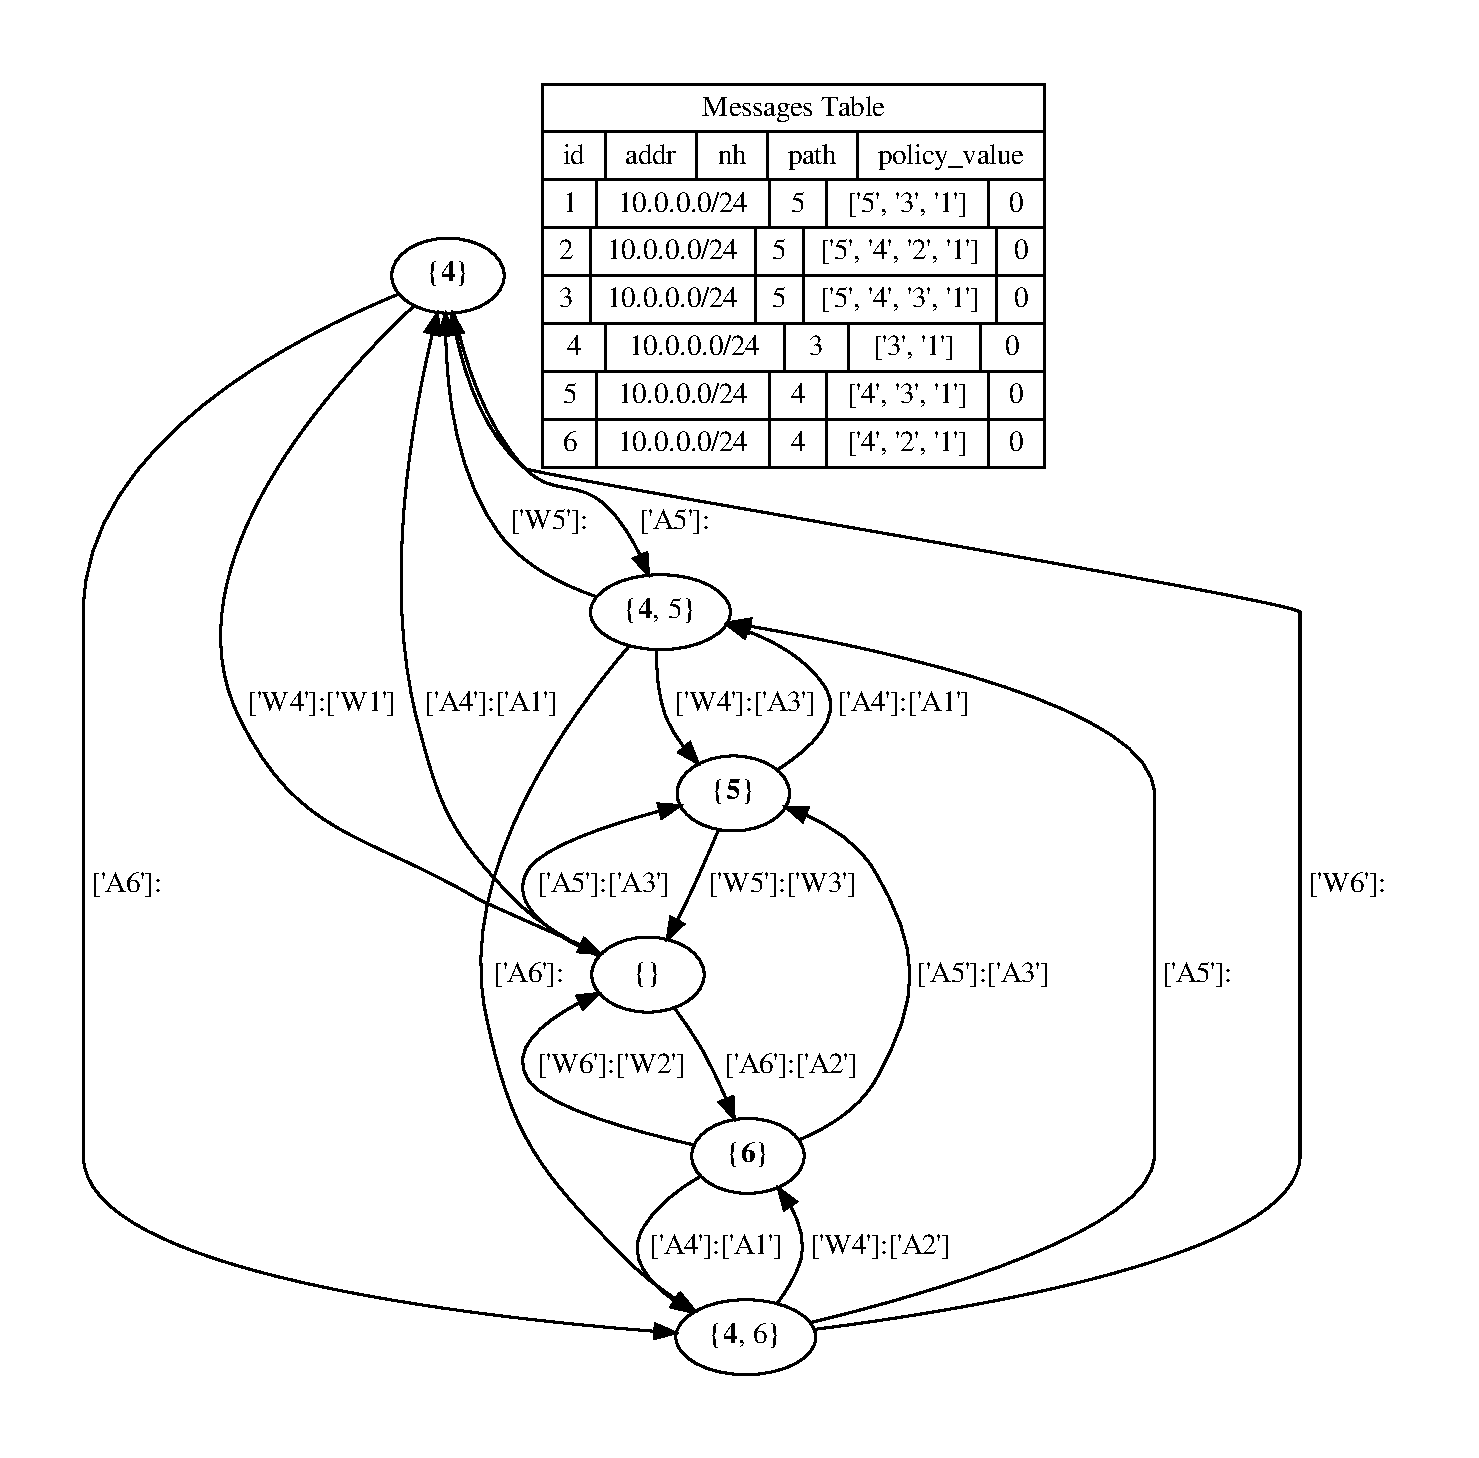
\includegraphics[width=\textwidth]{images/fsm/fig_4_5.pdf}
		 \caption{Node \num{5} \ac{CFSM} from the environment of \Cref{tbl:fig_4_example}}
         \label{fig:fsm_node5}
     \end{subfigure}
		\caption{\ac{CFSM} of nodes \num{4} and \num{5} of the graph \Cref{fig:griffin_fig_4} with an input signal of \q{AW}}
        \label{fig:fsm_griffin_fig4}
\end{figure}

The states of the \ac{CFSM} in \Cref{fig:fsm_griffin_fig4} are represented by the
knowledge of the nodes, composed by the routes that are in the \ac{RIB} of the node.
The bold value is the actual best route to the destination chosen by the node.
If in the state transition to a new state the best path is not affected then the
node will not transmit the new route to its neighbours, for an example take
a look to \Cref{fig:fsm_node4} from the state $\{1\}$ to the state $\{1, 3\}$
where the node \num{4} will learn a new route that is not the best one.

The effects of the implicit withdraw can be seen in \Cref{fig:fsm_node5}
the transition from $\{1, 4\}$ to $\{1, 3\}$ thanks to the reception of the
announcement $a3$ from the node \num{4}.

As written in \cite{griffinFSM}, I would like to underline the fact that, given
the \num{52} unique possible outputs of the node \num{5} it would be very difficult
to infer the initial signal that provokes all the transitions.

We can also analyze those output signals, having all the events for each single
run we can infer which were the most common output signals that a single node
experienced.
Is sufficient to take all the transmitted messages of a node and look the sequence
of advertisement and withdraws.

\begin{figure}[h]
     \centering
     \begin{subfigure}[b]{0.45\textwidth}
         \centering
         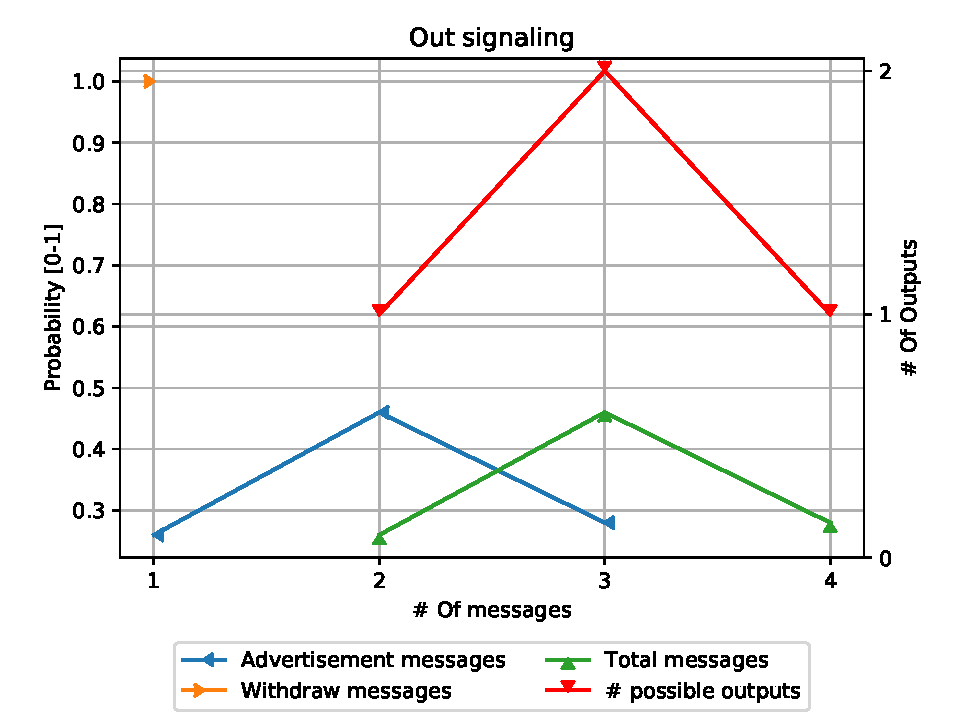
\includegraphics[width=\textwidth]{images/signal_study/fig_4/fig_4_4_signaling_nmessage_prob.pdf}
		 \caption{Node \num{4} output signals study}
         \label{fig:signal_node4}
     \end{subfigure}
     \hfill
     \begin{subfigure}[b]{0.45\textwidth}
         \centering
         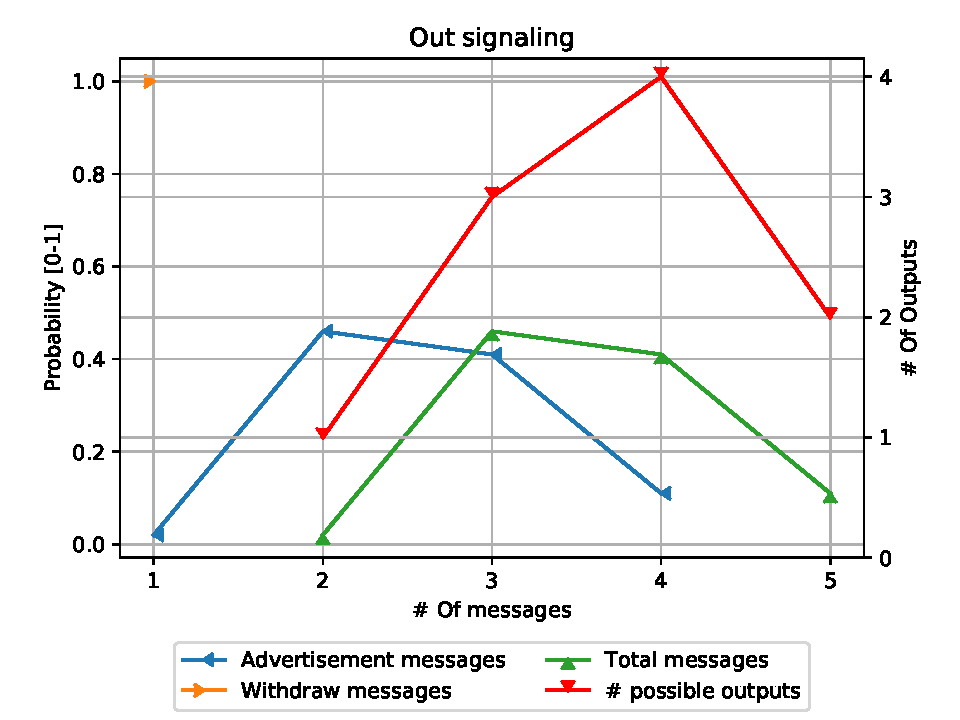
\includegraphics[width=\textwidth]{images/signal_study/fig_4/fig_4_5_signaling_nmessage_prob.pdf}
		 \caption{Node \num{5} output signals study}
         \label{fig:signal_node5}
     \end{subfigure}
		\caption{Output signal study of nodes \num{4} and \num{5} of the graph 
			\Cref{fig:griffin_fig_4} with an input signal of \q{AW} at node \num{1}}
        \label{fig:signal_griffin_fig4}
\end{figure}

The plots in \Cref{fig:signal_griffin_fig4} represents the probability of an
output signal of a certain length to appear and the number of unique output signals
of a unique length has been found.
The $x$ axis represents the number of messages in the output signal, a message
is a single announcement or withdraw.
The first $y$ axis represents the probability to see a certain number of messages
taking a random output signal from the output.
For this axis there are three lines that refer to it, the blue one represent the
number of advertisement messages in the output signal correlated with the 
respective probability.
For example, in \Cref{fig:signal_node4} there is a probability around $0.45$ to have
exactly two advertisement messages per output signal. And respectively a probability
slightly larger than $0.25$ to have only one advertisement or three.
We can also notice that we didn't see more than three advertisements or less than one.
The green line instead represents the total number of messages in the signal,
without distinguishing between advertisement and withdraws.
By the fact that we will always have one withdraw (the orange line) this line 
is simply shifted by one unit in respect of the advertisement line.
The second $y$ axis refers to the number of unique output signals encountered and
their length.
For example, in \Cref{fig:signal_node5} we will have \num{1} unique output signal
of length \num{2}, \num{3} signals of length \num{3} and \num{4} of length \num{4} and \num{2} of length \num{5}.

Those plots do not give a complete prospective of all the possible outputs
that can be generated but only the ones encountered during the runs.
In fact, during the \num{100} runs we encountered only the output signals listed
in \cref{tbl:signals}.

\begin{table}[h]
	\begin{subtable}[h]{0.45\textwidth}
		\begin{center}
	\begin{tabular}{ || m{3cm}| m{3cm} || } 
	\hline
	Signal & Frequency\\ 
	\hline \hline
		$a1a2a1w1$ & \num{28} \\
		$a2a1w1$ & \num{23} \\
		$a2w2$ & \num{26} \\
		$a1a2w2$ & \num{23} \\
	\hline
	\end{tabular}
\end{center}


		\caption{Node \num{4} output signals encountered}
		\label{tab:node4_outSignals}
    \end{subtable}
	\hfill
	\begin{subtable}[h]{0.45\textwidth}
		\begin{center}
	\begin{tabular}{ || m{3cm}| m{3cm} || } 
	\hline
	Signal & Frequency\\ 
	\hline \hline
	$a1a2a3w3$ & \num{15}\\
	$a1a3w3$ & \num{16}\\
	$a2a1a2w2$ & \num{19}\\
	$a1a2w2$ & \num{28}\\
	$a1w1$ & \num{2}\\
	$a2a1a3w3$ & \num{6}\\
	$a2a1a2a3w3$ & \num{8}\\
	$a3a1a2a3w3$ & \num{3}\\
	$a2a1w1$ & \num{2}\\
	$a3a1a3w3$ & \num{1}\\
	\hline
	\end{tabular}
\end{center}


		\caption{Node \num{5} output signals encountered}
		\label{tab:node5_outSignals}
    \end{subtable}
	\caption{Node 4 and 5 different output signals encountered during the runs}
	\label{tbl:signals}
\end{table}


\subsection{MRAI and BGP FSM}
\label{subsec:mrai_vs_bgpfsm}

How would \ac{MRAI} affect the study of the signals produced by \Cref{fig:griffin_fig_4}?
The answer is that the number of states will be the same but the number of possible
transitions will explode because there will be a lot more possible
input signals that will be compressed and evaluated by the nodes.

We can see the effects of \ac{MRAI} on the \ac{CFSM}s in \Cref{fig:fsm_griffin_fig4_MRAI}.

\fxfatal{\Cref{fig:fsm_node5_MRAI} is not readable at all, move the two figure
	one after the other}
\begin{figure}[h]
     \centering
     \begin{subfigure}[b]{0.45\textwidth}
         \centering
         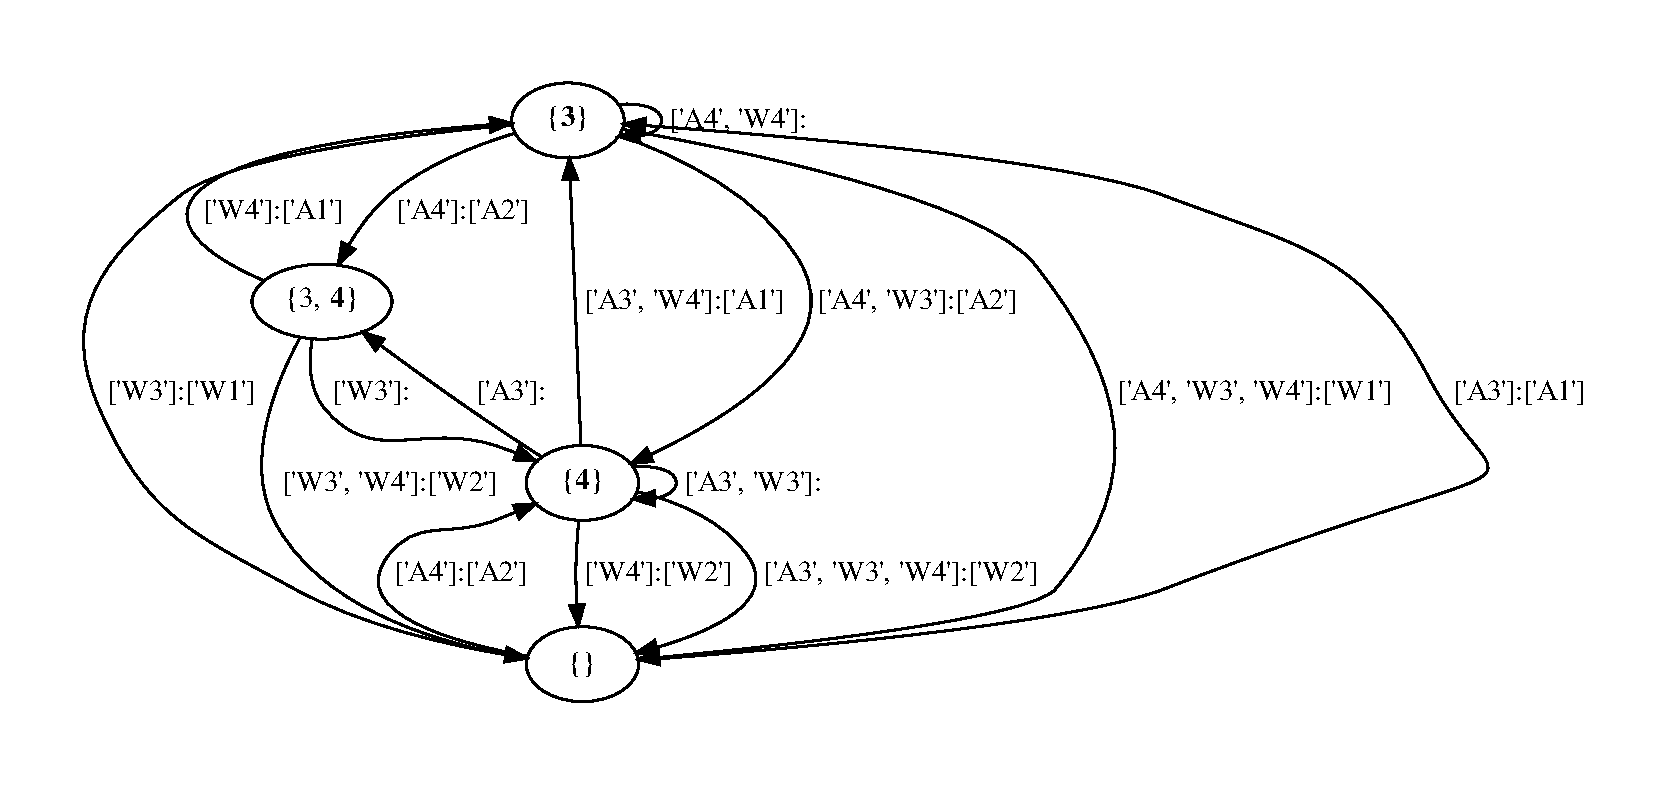
\includegraphics[width=\textwidth]{images/fsm/fig_4_4_MRAI30.pdf}
		 \caption{Node \num{4} \ac{CFSM} from the environment of \Cref{tbl:fig_4_example} with \ac{MRAI}=\SI{30}{\second}}
         \label{fig:fsm_node4_MRAI}
     \end{subfigure}
     \hfill
     \begin{subfigure}[b]{0.45\textwidth}
         \centering
         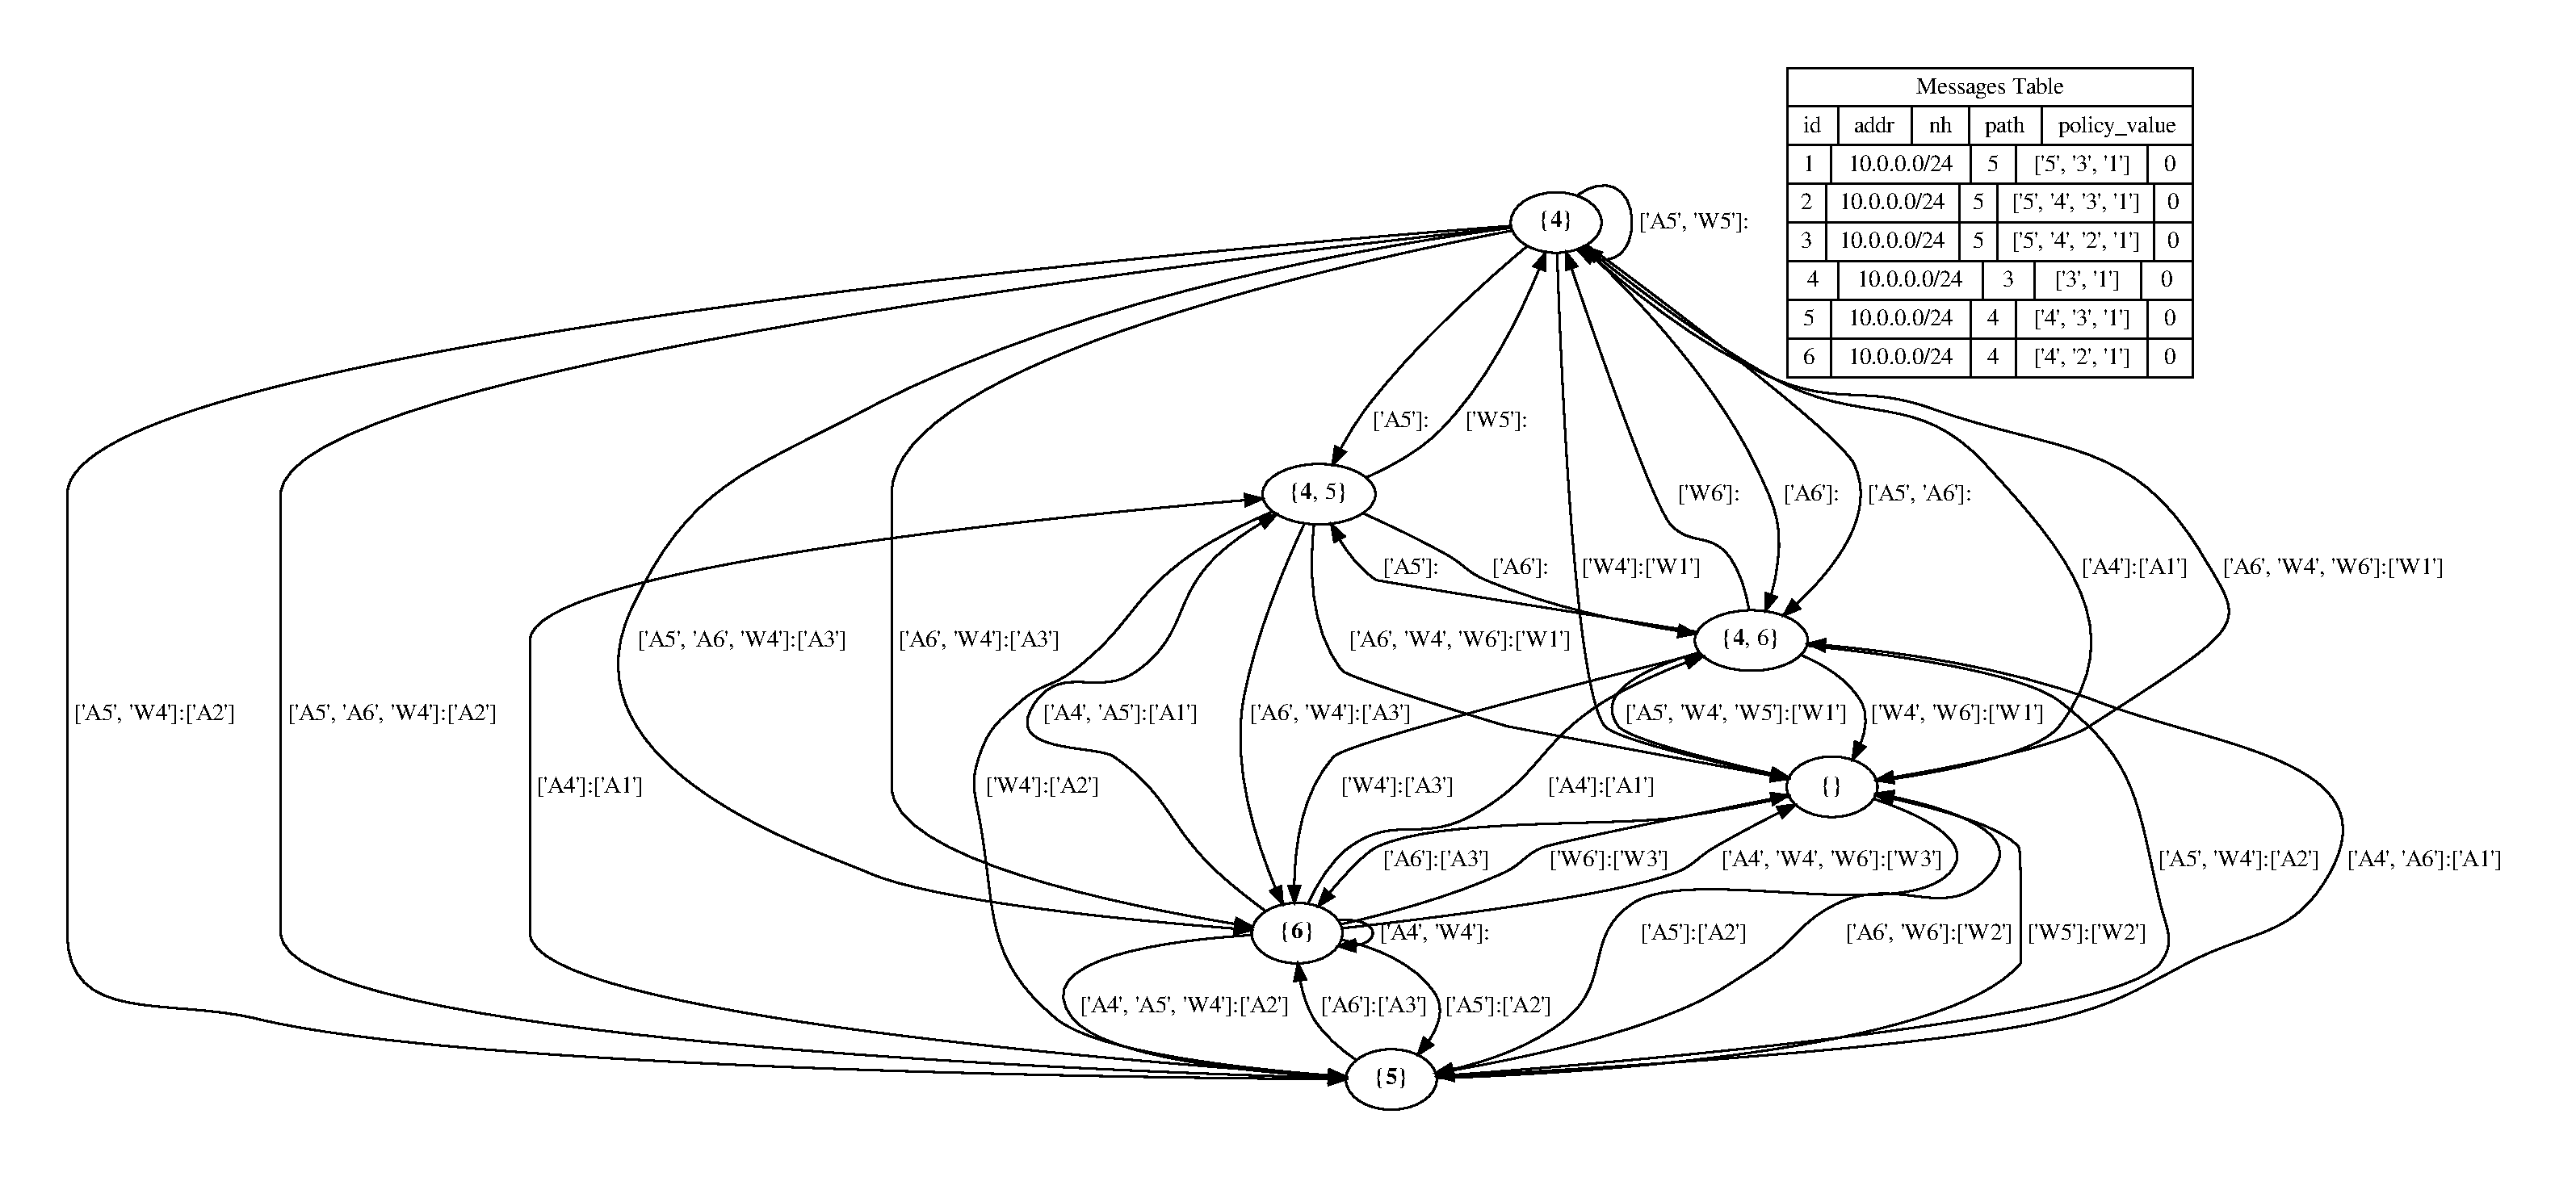
\includegraphics[width=\textwidth]{images/fsm/fig_4_5_MRAI30.pdf}
		 \caption{Node \num{5} \ac{CFSM} from the environment of \Cref{tbl:fig_4_example} with \ac{MRAI}=\SI{30}{\second}}
         \label{fig:fsm_node5_MRAI}
     \end{subfigure}
		\caption{\ac{CFSM} of nodes \num{4} and \num{5} of the graph 
			\Cref{fig:griffin_fig_4} with an input signal of \q{AW} with
			\ac{MRAI}=\SI{30}{\second}}
        \label{fig:fsm_griffin_fig4_MRAI}
\end{figure}

\Cref{fig:fsm_node4} and \Cref{fig:fsm_node4_MRAI} permits us to compare the two
\ac{CFSM}s of node \num{4} and is possible to nice a big difference in terms of edges
between one figure and the other, the first one has \num{8} transitions, the
second one \num{15}.
For the node \num{5} we pass from \num{16} transitions to \num{36}.

But the positive effects of \ac{MRAI} can be found in the output signals, 
showed in \Cref{fig:signal_griffin_fig4_MRAI}.

\begin{figure}[h]
     \centering
     \begin{subfigure}[b]{0.45\textwidth}
         \centering
         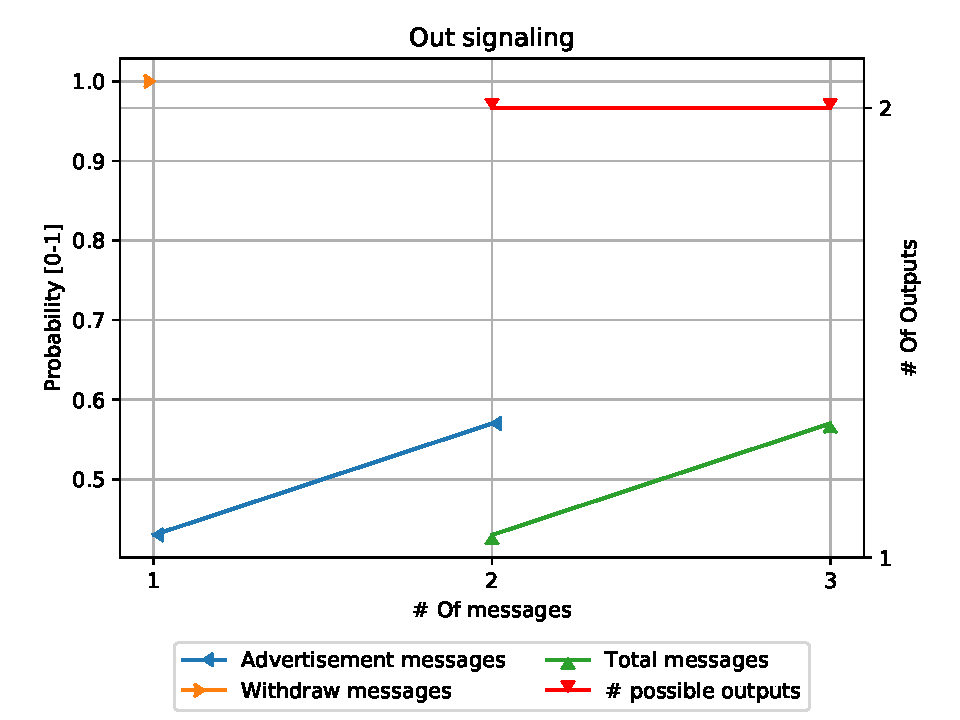
\includegraphics[width=\textwidth]{images/signal_study/fig_4_MRAI/fig_4_4_signaling_nmessage_prob.pdf}
		 \caption{Node \num{4} output signals study with \ac{MRAI}=\SI{30}{\second}}
         \label{fig:signal_node4_MRAI}
     \end{subfigure}
     \hfill
     \begin{subfigure}[b]{0.45\textwidth}
         \centering
         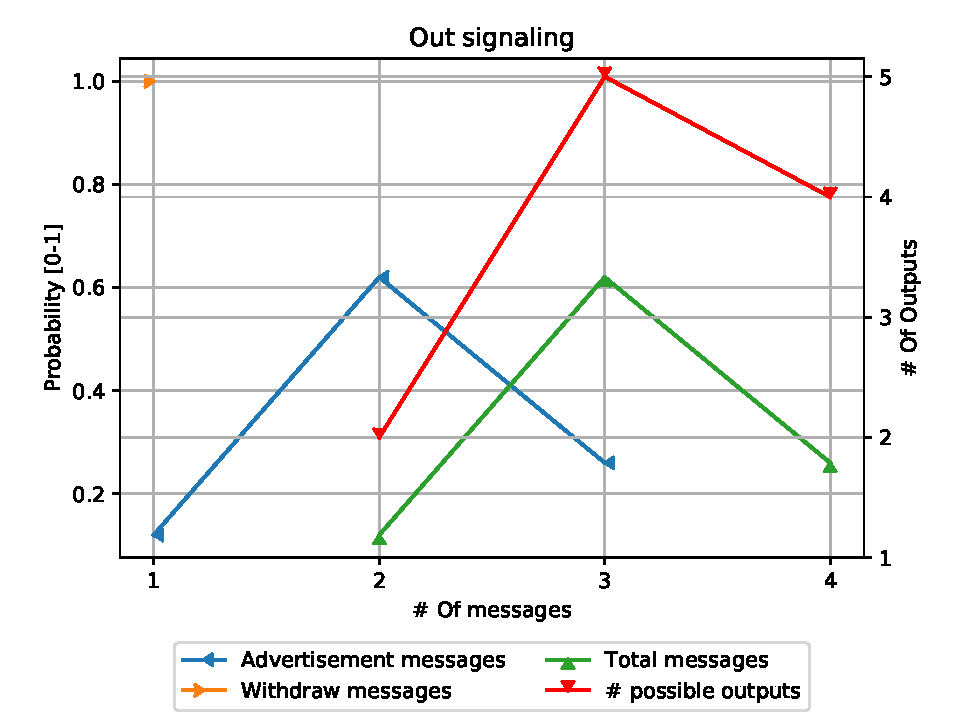
\includegraphics[width=\textwidth]{images/signal_study/fig_4_MRAI/fig_4_5_signaling_nmessage_prob.pdf}
		 \caption{Node \num{5} output signals study with \ac{MRAI}=\SI{30}{\second}}
         \label{fig:signal_node5_MRAI}
     \end{subfigure}
		\caption{Output signal study of nodes \num{4} and \num{5} of the graph 
			\Cref{fig:griffin_fig_4} with an input signal of \q{AW} at node \num{1}
			with \ac{MRAI}=\SI{30}{\second} for every link}
        \label{fig:signal_griffin_fig4_MRAI}
\end{figure}

Comparing \Cref{fig:signal_node5_MRAI,fig:signal_node5} is possible to notice
that there is a different distribution of output signals.
The $x$ axis never reach the value of \num{5}, this means that the output signals
of the node \num{5} never used more than \num{4} messages.
And we can also notice that the majority of the signals this time have a length
of \num{3} messages, instead of the previous \num{4}.
This is a hint that \ac{MRAI} can have positive effects on the number of output messages
produced by single nodes, having, however, more possible transitions to consider.

\section{BGP FSM explosion}
\label{sec:bgp_fsm_explosion}

We know that \ac{MRAI} is not an easy parameter, the incorrect setting of
it can lead to an explosion of messages and an exponential convergence time.
This problem has been studied by Fabrikant et al. \cite{fabrikant2011there} and
the origin of the problem has been attributed to the \textit{path exploration}
problem.
This is a well-known problem in the \ac{BGP} community and it is experienced
by a node when it enters in a transitory phase where it accepts and publishes not
optimal paths towards the destination before reaching a stable state.
\textit{Path exploration} can lead to an enormous amount of messages even with
a small set of nodes \cite{deshpande2004impact}.

As we saw in \Cref{subsec:mrai_vs_bgpfsm} that \ac{MRAI} can influence the
\ac{CFSM}s of the nodes and their output signals, which impact could it have
if it is not set correctly?

I have then created an environment that resembles the study conducted by
\cite{fabrikant2011there} using a topology like the one described in \Cref{subsec:fabrikant_env}
with \num{3} rings.
with different \ac{MRAI} settings.
The environment properties are presented in \Cref{tbl:fabrikant_environment}.

\begin{table}[h]
	\begin{center}
	\begin{tabular}{ || m{4cm}| m{7.5cm} || }
	\hline
	Property & Value \\
	\hline \hline
	Seeds & $[1, 30]$ \\
	\hline
		Signaling & \q{A}, \q{AW}, \q{AWA}, \q{AWAW} \\
	\hline
		Withdraws delay & Uniform distribution between \SI{5}{\second} and \SI{10}{\second}, Uniform distribution between \SI{10}{\second} and \SI{15}{\second} \\
	\hline
	Announcement delay & Uniform distribution between \SI{5}{\second} and \SI{10}{\second}, Uniform distribution between \SI{10}{\second} and \SI{15}{\second} \\
	\hline
	Link delay & Uniform distribution between \SI{0.5}{\second} adn \SI{3}{\second}, uniform distribution between \SI{2}{\second} and \SI{4}{\second} \\
	\hline
	\end{tabular}
\end{center}

	\caption{Fabrikant experiments environment}
	\label{tbl:fabrikant_environment}
\end{table}

In total, for each signaling experiment this environment produces \num{240} runs.
I have then introduced \num{4} different \ac{MRAI} strategies for each different
signal.
The different \ac{MRAI} strategies are the following one:
\begin{itemize}
	\item \textbf{\textit{Fixed \SI{30}{\second}}}: \ac{MRAI} is fixed for each link to \SI{30}{\second};
	\item \textbf{\textit{No \ac{MRAI}}}: \ac{MRAI} is fixed for each link to \SI{0.0}{\second};
	\item \textbf{\textit{Ascendant}}: \ac{MRAI} will be doubled at each leach (1 − 2 − 4 − 8 − ...);
	\item \textbf{\textit{Descendent}}: Reverse of the ascendant case, \ac{MRAI} will be divided by two at each leach.
\end{itemize}

Another important factor to consider during those experiments is the \ac{IW}
capability of \ac{BGP}.
This parameter will influence the number of messages
that will be transmitted.

The results of all those different experiments, in terms of \ac{CFSM} are
exposed in \Cref{tbl:fabrikant_cfsm}

\begin{table}[h]
	\centering
\begin{tabular}{||c|c|c|c|c|c|c|c|c|c||}
	\hline
\multirow{2}{*}{Signaling} & \multirow{2}{*}{IW} & \multicolumn{2}{c|}{No MRAI} & \multicolumn{2}{c|}{Fixed 30s} & \multicolumn{2}{c|}{Ascendent} & \multicolumn{2}{c||}{Descendent} \\
	\cline{3-10}
                           &                     & $|S|$          & $|T|$          & $|S|$           & $|T|$           & $|S|$           & $|T|$           & $|S|$            & $|T|$           \\
	\hline
	\hline
	                            & Yes                  & 12                         & 19                          & 15    & \cellcolor[HTML]{C0C0C0}26 & 7              & 12            & \cellcolor[HTML]{C0C0C0}16 & 24                          \\ \cline{2-10}
	\multirow{-2}{*}{\q{A}}         & No                   & 30                         & 100                         & 30    & 125                        & 9              & 21            & 30                         & \cellcolor[HTML]{C0C0C0}132 \\ \hline
                            & Yes                  & \cellcolor[HTML]{C0C0C0}52 & \cellcolor[HTML]{C0C0C0}181 & 37    & 103                        & 24             & 71            & 40                         & 80                          \\ \cline{2-10}
	\multirow{-2}{*}{\q{AW}}        & No                   & 51                         & 221                         & 57    & 263                        & 22             & 90            & \cellcolor[HTML]{C0C0C0}58 & \cellcolor[HTML]{C0C0C0}274 \\ \hline
                            & Yes                  & \cellcolor[HTML]{C0C0C0}51 & \cellcolor[HTML]{C0C0C0}170 & 25    & 50                         & 33             & 148           & 50                         & 137                         \\ \cline{2-10}
	\multirow{-2}{*}{\q{AWA}}       & No                   & \cellcolor[HTML]{C0C0C0}69 & 364                         & 37    & 180                        & 30             & 203           & 66                         & \cellcolor[HTML]{C0C0C0}419 \\ \hline
                            & Yes                  & \cellcolor[HTML]{C0C0C0}77 & \cellcolor[HTML]{C0C0C0}461 & 38    & 132                        & 54             & 300           & 53                         & 148                         \\ \cline{2-10}
	\multirow{-2}{*}{\q{AWAW}}      & No                   & \cellcolor[HTML]{C0C0C0}78 & \cellcolor[HTML]{C0C0C0}500 & 62    & 429                        & 48             & 350           & 66                         & 441                         \\ \cline{2-10}
	\hline
\end{tabular}

	\caption{Fabrikant \ac{CFSM}s results, $|S|$ is the dimension of the states set
		$|T|$ is the dimension of the transitions set, The worst results for each
		category are colored in gray, the topology contains \num{3} rings, as
		\Cref{fig:fabrikant_graph}}
	\label{tbl:fabrikant_cfsm}
\end{table}

As is possible to see from the grey squares in \Cref{tbl:fabrikant_cfsm} the more
complex \ac{CFSM}s are the ones without \ac{MRAI} and with a descendent \ac{MRAI}
timing.
The second case is the same described in \cite{fabrikant2011there} and the extremely
high number of transitions is caused by the \textit{Path Exploration} problem.
Is also noticeable that the \ac{IW} has a huge effect on both the number
of states and the number of transitions.
This because there are less possible combinations of input signals for the nodes.
The opposite case in respect of the \textit{Descendent} strategy obtains
great results, even better than the actual standard of \SI{30}{\second} for
each link.
This performance improvement is caused by the fact that each leach will wait
enough time to have more information from its predecessor in order to have
more information to make the best decision.

The \textit{Path Exploration} problem is also noticeable evaluating the
output signals of the last node of the chain.
Results about the output signal of the node \num{8} (the last node of the gadget)
are presented in \Cref{fig:signal_fabrikant}.

\begin{figure}[ht]
     \centering
     \begin{subfigure}[b]{0.32\textwidth}
         \centering
         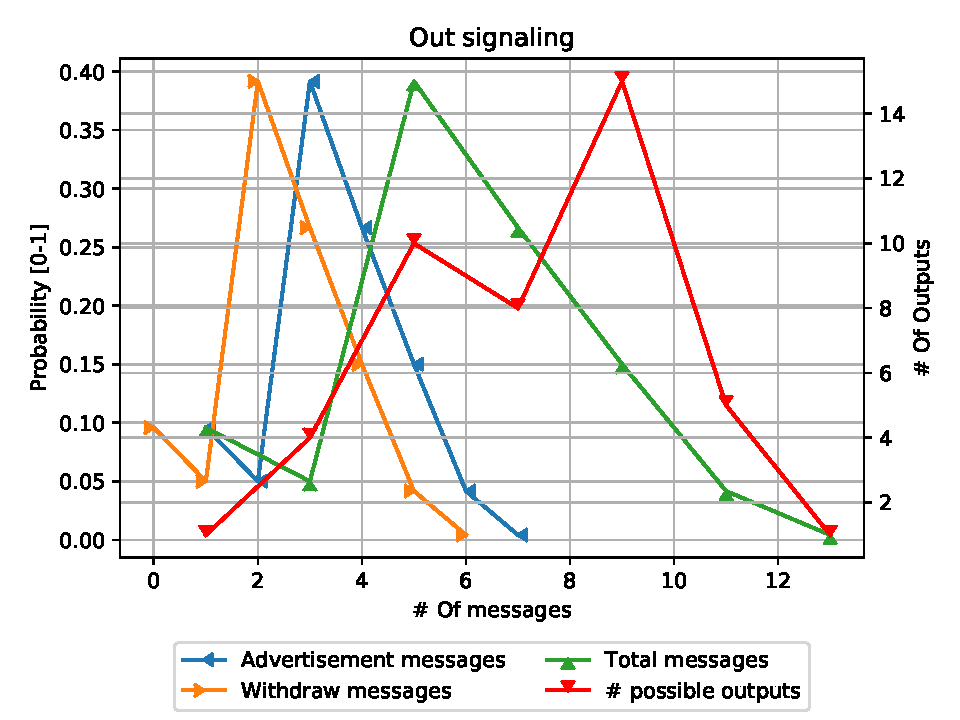
\includegraphics[width=\textwidth]{images/signal_study/fabrikant/30Fixed.pdf}
		 \caption{Node \num{8} output signals study with \textbf{\textit{Fixed \SI{30}{\second}}} strategy}
         \label{fig:signal_node9_fabrikant_fixed30_noIW}
     \end{subfigure}
     \hfill
     \begin{subfigure}[b]{0.32\textwidth}
         \centering
         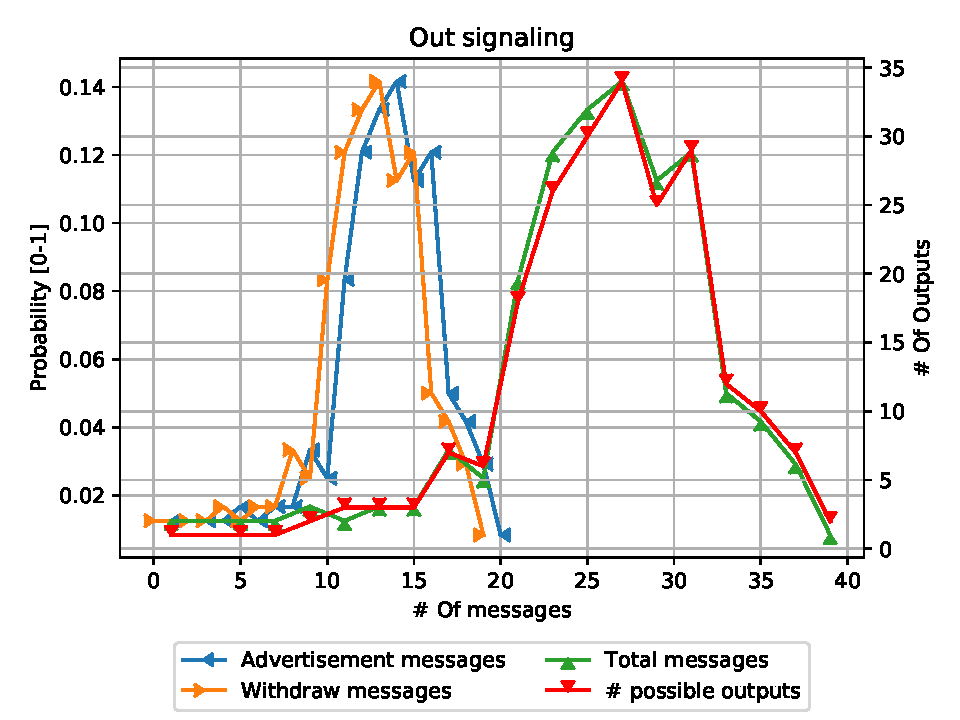
\includegraphics[width=\textwidth]{images/signal_study/fabrikant/Descendent.pdf}
		 \caption{Node \num{9} output signals study with \textbf{\textit{Descendent}} strategy}
         \label{fig:signal_node9_fabrikant_descendent_noiw}
     \end{subfigure}
     \hfill
     \begin{subfigure}[b]{0.32\textwidth}
         \centering
         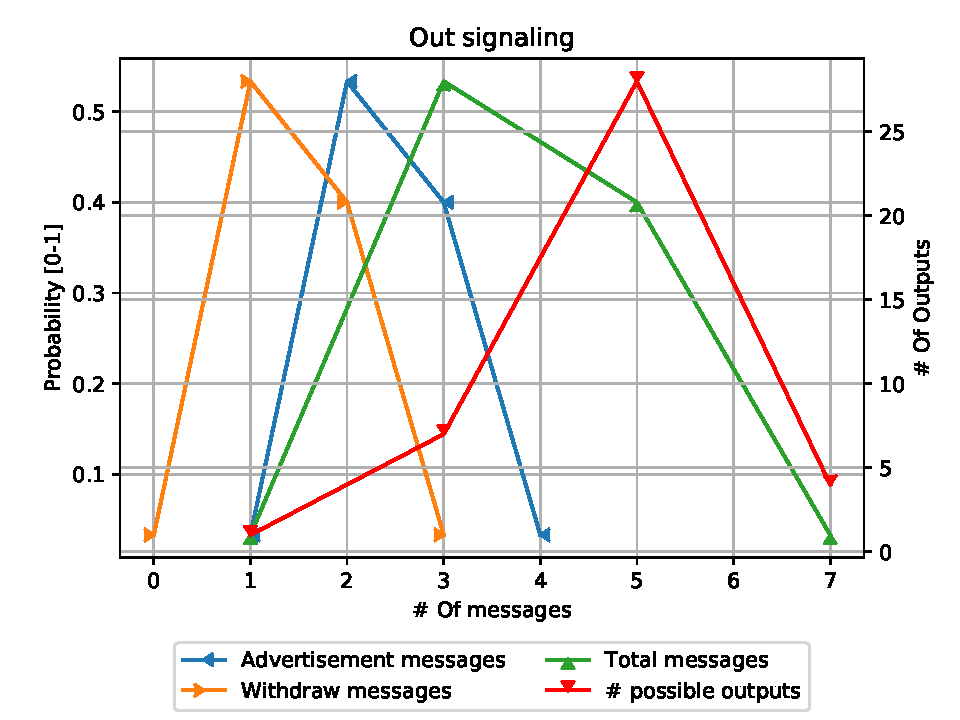
\includegraphics[width=\textwidth]{images/signal_study/fabrikant/Ascending.pdf}
		 \caption{Node \num{9} output signals study with \textbf{\textit{Ascendant}} strategy}
         \label{fig:signal_node9_fabrikant_ascendent_noIW}
     \end{subfigure}
		\caption{Output signal study of nodes \num{8} of the graph 
			\Cref{fig:fabrikant_graph} with an input signal of \q{AWA} at node $d$
			with the \textbf{\textit{Fixed \SI{30}{\second}}}, \textbf{\textit{Descendent}}
			and \textbf{\textit{Ascendant}}	strategies, without the help of the \ac{IW}}
        \label{fig:signal_fabrikant}
\end{figure}

The first signal study, \Cref{fig:signal_node9_fabrikant_fixed30_noIW} is the
one that represents the actual standard of the protocol \cite{rfc4271}.
We can notice in that particular output study that the maximum detected length of
a signal is \num{13} and it's the last probable output, while the most probable
output length is \num{5}.
While we can notice the \textit{Path Exploration} problem by the spike of unique
output signals with a length of \num{9}, this mean that the node experienced some
changes in its decisions.
The worst-case scenario is the one represented by \cref{fig:signal_node9_fabrikant_descendent_noiw}
where the maximum length of the output signal reaches almost \num{40} messages, but
the most probable output signal has a length between \num{20} and \num{30}.
This is the marker of a lot of decision changes in the best path for the node \num{8}.
Opposite to that case, we found the \textit{Ascendent} strategy in 
\Cref{fig:signal_node9_fabrikant_ascendent_noIW} where the number of output
signals never used more than \num{7} messages.
The node \num{8} in this last case almost never experienced the \textit{Path Exploration}
problem, thanks to the fact that most of the times the information it receives
from the neighbourhood are already corrected.

In conclusion of this chapter, we can say without doubts that \ac{MRAI} influences
the number of states experienced by a node and, confirming what has been sad in
\cite{fabrikant2011there}, that an incorrect setting of it can lead
to an explosion on the number of states and transitions.
It is also noticeable that a different setting of \ac{MRAI} can also lead
to a better scenario than the standard one.
Alternatives to the standard \ac{MRAI} has been already presented \fxfatal{Include
citations and maybe find a better end of the chapter}

    \chapter{BGP MRAI dependency}
\label{cha:bgp_mrai_experiments}

\ac{MRAI} is one of the parameters that mostly has caused divergences in the 
scientific community.
And, after the introduction in the protocol since version 4 \cite{rfc4271}
\fxfatal{Check this sentence}, is one of the more studied for the possibility
to improve the protocol or generate exponential convergence behaviour in small
network \cite{fabrikant2011there}.

The protocol strictly depends on this parameter, because as we saw in \Cref{cha:bgp_fsm},
the incorrect use of it can lead to tremendous consequences, even worst of not
having it at all.
In other cases, with a particular setting of it is possible to improve the network
performances.
Recent studies about centrality metrics on routing protocols introduce, through 
the distributed computation of the metric, to a 
timer trade-off improvement \cite{MaLo18_ToN,GhiMa18_infocom}.
This kind of approach has been also applied on \ac{BGP} with positive results on
network failures \cite{milani2019BGP,milani2020improving}.

All those study points out how we can set \ac{MRAI} to improve network
performances, but what about how \ac{MRAI} reacts on different problems?
Is it possible that \ac{MRAI} reacts differently based on where the signal
occurs?
In fact, our hypothesis is that is not enough just look to the \ac{MRAI} setting
because also other factors can be relevant.
For example, a change near the central clique of $T$ nodes could provoke a large
storm of messages because \ac{MRAI} doesn't affect in time the spreading of information.
While, a change in the periphery could be cushioned without it reaching the center
of the network.

\section{Clique graph}
\label{sec:bgp_mrai_clique}

The clique topology is one of the worst-case scenarios as specified in Labovitz et al.
\cite{labovitz2000delayed}
I used two approaches in this Environment, the first one keeps the \ac{IW} active
the second one doesn't use of this property.
To emphasize the effects of this parameter with the effects also of different 
\ac{MRAI} settings.

The Environment properties are listed in \Cref{tbl:clique_properties}

\begin{table}[h]
	\begin{center}
	\begin{tabular}{ || m{4cm}| m{8cm} || } 
	\hline
	Property & Value \\ 
	\hline \hline
	Seeds & $[1, 10]$ \\ 
	\hline
	Signaling & \q{AW} \\
	\hline
		Withdraws delay & Uniform distribution between \SI{1}{\second} and \SI{5}{\second} \\ 
	\hline
	Announcement delay & constant distribution of \SI{5}{\second} \\ 
	\hline
		MRAI & $[0, 60]$ \\
	\hline
	Link delay & Uniform distribution between \SI{0.0001}{\second} and \SI{0.5}{\second} \\
	\hline
	\end{tabular}
\end{center}

	\caption{Clique environment properties}
	\label{tbl:clique_properties}
\end{table}

As described in \Cref{tbl:clique_properties}, for each \ac{MRAI} value has been
executed \num{10} different runs of the environment.
The clique graph used in this experiments is composed by \num{15} nodes.
The \ac{MRAI} strategy used is the \textit{fixed}, so every link will have the
same \ac{MRAI} value.
The results are presented in \Cref{fig:clique_evolution}

\begin{figure}[h]
     \centering
     \begin{subfigure}[b]{0.45\textwidth}
         \centering
         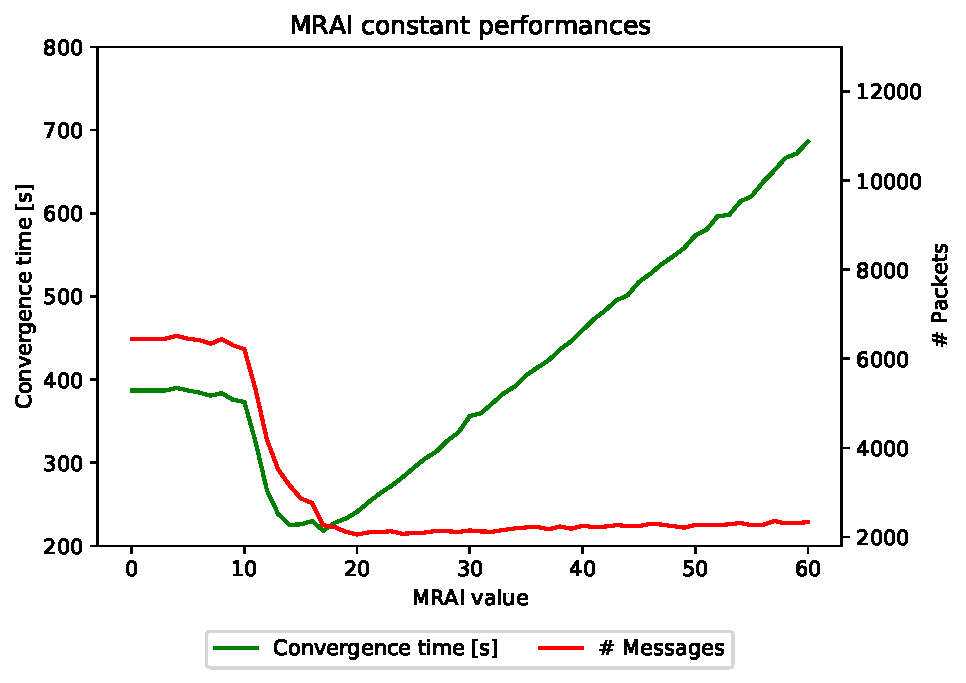
\includegraphics[width=\textwidth]{images/clique/messagesVStime/pareto-clique-constant_mrai_evolution.pdf}
		 \caption{Network performances \textbf{with} \textbf{\ac{IW}}}
         \label{fig:clique_evolution_IW}
     \end{subfigure}
     \hfill
     \begin{subfigure}[b]{0.45\textwidth}
         \centering
         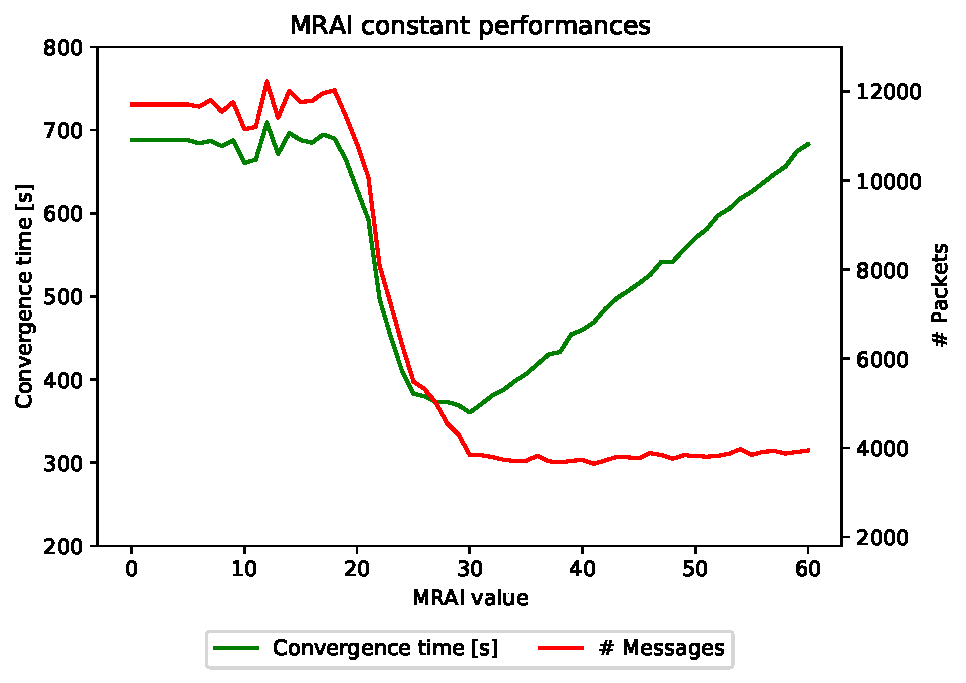
\includegraphics[width=\textwidth]{images/clique/messagesVStime/pareto-clique-noIW-constant_mrai_evolution.pdf}
		 \caption{Network performances \textbf{without} \textbf{\ac{IW}}}
         \label{fig:clique_evolution_noIW}
     \end{subfigure}
		\caption{Evolution of the network performances on the clique graph of \num{15}
			nodes using a fixed \ac{MRAI} from \num{0} to \num{60} seconds. \fxfatal{
			use the same interval in the y-axis?}}
        \label{fig:clique_evolution}
\end{figure}

Is possible to notice in \Cref{fig:clique_evolution} both the effect of \ac{MRAI}
and \ac{IW}.
Those plots represent the network performances in terms of convergence time and
number of messages transmitted to reach the convergence after the transmission 
of the signal \q{AW}.
The convergence time is represented by the average time from all the nodes in the 
network.
Each point in the plots is the average of the \num{10} runs with the \textit{fixed}
\ac{MRAI} value on the $x$ axis.
The left $y$ axis should be used with the convergence time, the green line, while
the second $y$ axis represents the number of messages transmitted, the red line.

The effects of the first one are present in both the plots but in two different
moments.
In \Cref{fig:clique_evolution_IW} \ac{MRAI} affects both the convergence time and
the number of messages around \SI{20}{\second} up to \SI{30}{\second}.
After the threshold of \SI{30}{\second}, the effects of \ac{MRAI} are counterproductive,
the convergence time is negatively affected because the nodes start to wait more
time without obtaining more useful information.
This can be seen also in the number of messages that reaches a constant value.

In \Cref{fig:clique_evolution_noIW} we can see the same effect but with a higher
\ac{MRAI} value.
The number of transmitted messages reaches the constant value with an \ac{MRAI}
value around \SI{30}{\second}.
The effects of \ac{IW} can be saw also in the number of messages and the convergence
time with a low \ac{MRAI}, is possible to reach even \num{12000} messages while
with \ac{IW} the maximum value is around \num{6500} messages.


\section{Internet like graph}
\label{sec:bgp_mrai_internet_like}

The internet like environment is more complex than the clique one, but it permits
to have a more close vision of what can really happen on the Internet.
During my studies, I used different topologies with \num{1000} nodes resembling 
the Elmokashfi properties \cite{elmokashfi2010scalability} already 
described in \Cref{subsec:internet_like_env}.

Using this graph I will look for a possible correlation between \ac{MRAI} and other
factors that can influence the network.
First of all \ac{MRAI} has a dependence on how it is set, I'm going to compare
different \ac{MRAI} strategies that can be used on an Internet-like graph.
Another influencing factor could be the signal used as an input or even the position 
of the node that provoke the change.

\section{Strategy dependence}
\label{sec:bgp_mrai_strategy_dependance}

Like I mentioned before, the network performances depend on the \ac{MRAI} strategies
chosen.
For this reason, the first goal of my study is to point out these differences.
In order to do that, the first study that I would like to present is the one
that studies how the standard protocol evolves on an Internet environment.

The property of the environment chosen are described in \Cref{tbl:internet_like_properties}

\begin{table}[h]
	\begin{center}
	\begin{tabular}{ || m{4cm}| m{8cm} || } 
	\hline
	Property & Value \\ 
	\hline \hline
	Seeds & $[1, 10]$ \\ 
	\hline
	Signaling & \q{AW} \\
	\hline
		Withdraws delay & Uniform distribution between \SI{1}{\second} and \SI{60}{\second} \\ 
	\hline
	Implicit withdraw & Active \\ 
	\hline
		MRAI & $[0, 60]$ \\
	\hline
	Link delay & Uniform distribution between \SI{0.012}{\second} and \SI{3}{\second} \\
	\hline
	\end{tabular}
\end{center}

	\caption{Internet like environment properties}
	\label{tbl:internet_like_properties}
\end{table}

The graph is an \textit{Internet-like} graph with \num{1000} nodes.
The node that will execute the signal has been chosen randomly between 
all the nodes of type \q{C}.
This graph will be the same for all the experiments in this section.

For each \ac{MRAI} strategy, that I'm going to present, has been executed \num{61}
experiments, one for each possible value of \ac{MRAI}, for each experiments
thanks to the environment variable has been executed \num{10} runs.
In total for each \ac{MRAI} strategy has been run \num{610} different runs

As \ac{MRAI} strategies I decided to use the following two:
\begin{itemize}
	\item \textbf{\textit{Fixed}}; Every link will have the same
		\ac{MRAI} value;
	\item \textbf{\textit{DPC}}; This strategy assign a different 
		\ac{MRAI} value to each link depending on the centrality of the node \cite{milani2020improving}
\end{itemize}

The centrality metric used is called \ac{DPC} and thanks to the fact that has been
already demonstrated that is possible to calculate it in a distributed way \cite{milani2019BGP} I will
assume that it is calculated in advance and that every node knows it's own centrality to
set the timers.

To permit a comparison between those two different strategies a constraint on the
\ac{MRAI} assignment has been introduced, the $mean$ of all the timers in the network
must be equal between the two strategies.
For the \textit{Fixed} strategy, this is constraint intrinsically respected.
For the \textit{DPC} strategy, the timers are multiplied by a factor $k$ that
permits to keep the average equal.

The results of the first strategy are showed in \Cref{fig:internet_like_1000_constant_evolution}.

\begin{figure}[h]
     \centering
     \begin{subfigure}[b]{0.45\textwidth}
         \centering
         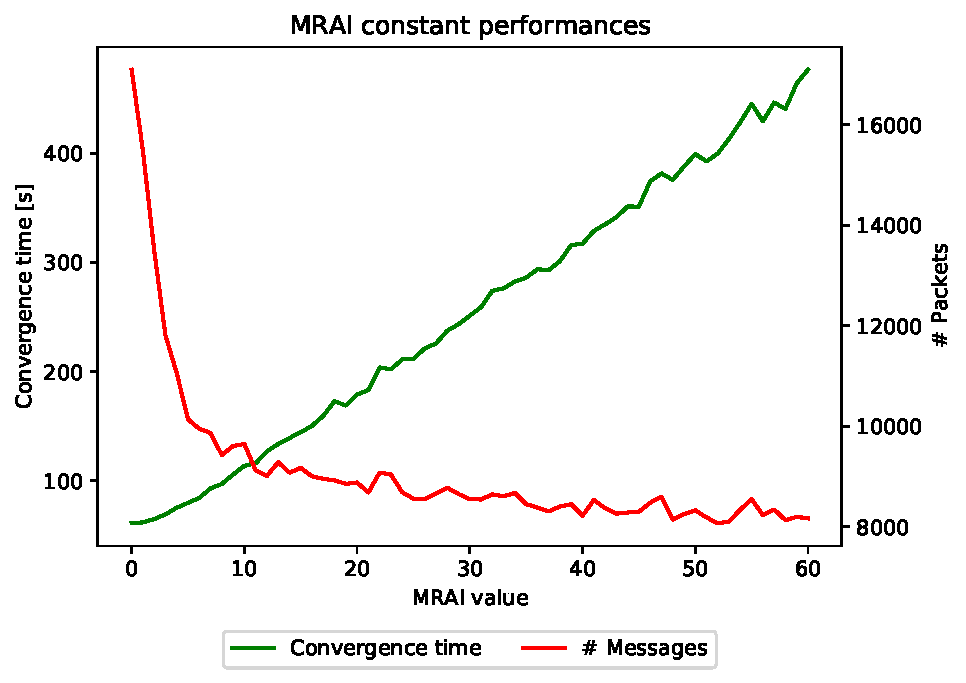
\includegraphics[width=\textwidth]{images/internet_like/1000/constantMRAI/internet_like-constant_mrai_evolution.pdf}
		 \caption{Network performances, messages VS convergence time with different
			\ac{MRAI} values}
         \label{fig:internet_like_1000_constant_evolution_evolution}
     \end{subfigure}
     \hfill
     \begin{subfigure}[b]{0.45\textwidth}
         \centering
         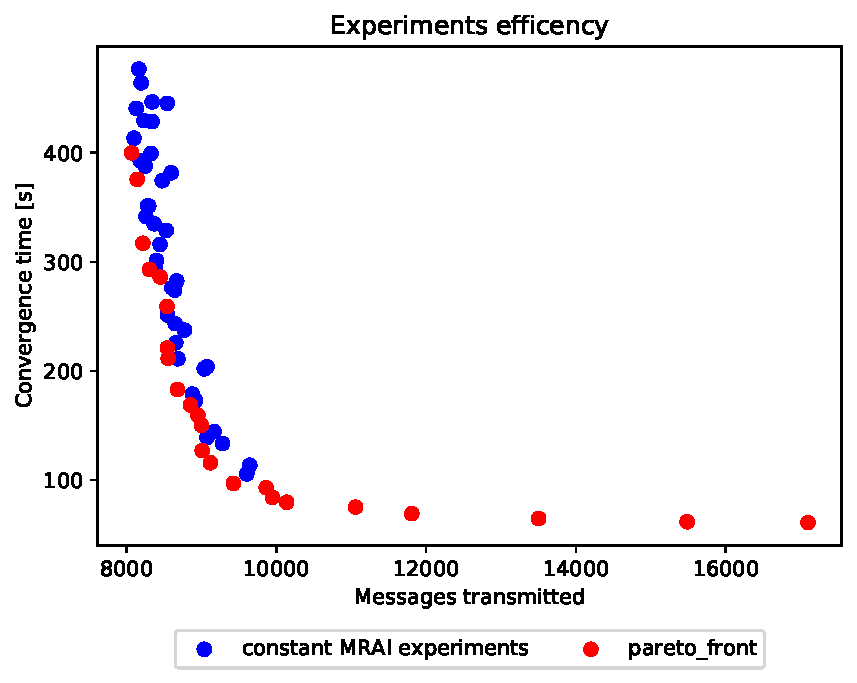
\includegraphics[width=\textwidth]{images/internet_like/1000/constantMRAI/internet_like-constant.pdf}
		 \caption{Pareto front of Messages VS Convergence time}
         \label{fig:internet_like_1000_constant_evolution_paretoFront}
     \end{subfigure}
		\caption{Evolution of the network performances on the \textbf{Internet Like} graph 
			of \num{1000} nodes using a fixed \ac{MRAI} from \num{0} to \num{60} seconds.}
        \label{fig:internet_like_1000_constant_evolution}
\end{figure}

As is possible to see in \Cref{fig:internet_like_1000_constant_evolution_evolution}
without \ac{MRAI} we would have a low convergence time, dictated mostly by 
network delays and processing time. With, on the other hand, an enormous amount
of messages.
Slightly increasing the \ac{MRAI} value, the number of messages will fell down
reaching a constant value around \num{8000}, while the convergence time
continuously grows linearly, as it happened for the clique graph in \Cref{fig:clique_evolution}.
This continuous linear grow is dictated by the fact that nodes keep meaningful
information for more time before sharing them with their neighbourhood.
\Cref{fig:internet_like_1000_constant_evolution_paretoFront} represent the Pareto
front of those experiments.
The Pareto frontier is the set of values that are Pareto efficient, this concept
has been already used in engineering to define the set of best outcomes from
the trade-off of two different parameters \cite{goodarzi2014introduction}.
We can clearly see that the majority of the points is concentrated on the left
of the chart, this means that few \ac{MRAI} values would give as a result
a high number of messages and a small convergence time.
While multiple \ac{MRAI} values would concentrate around the same value of 
messages transmitted.
This can confirm the fact that \ac{MRAI} would not influence messages
after a certain threshold but only the convergence time.

The results of the same environment without \ac{IW} are showed in 
\Cref{fig:internet_like_1000_constant_evolution_noIW}.

\begin{figure}[h]
     \centering
     \begin{subfigure}[b]{0.45\textwidth}
         \centering
         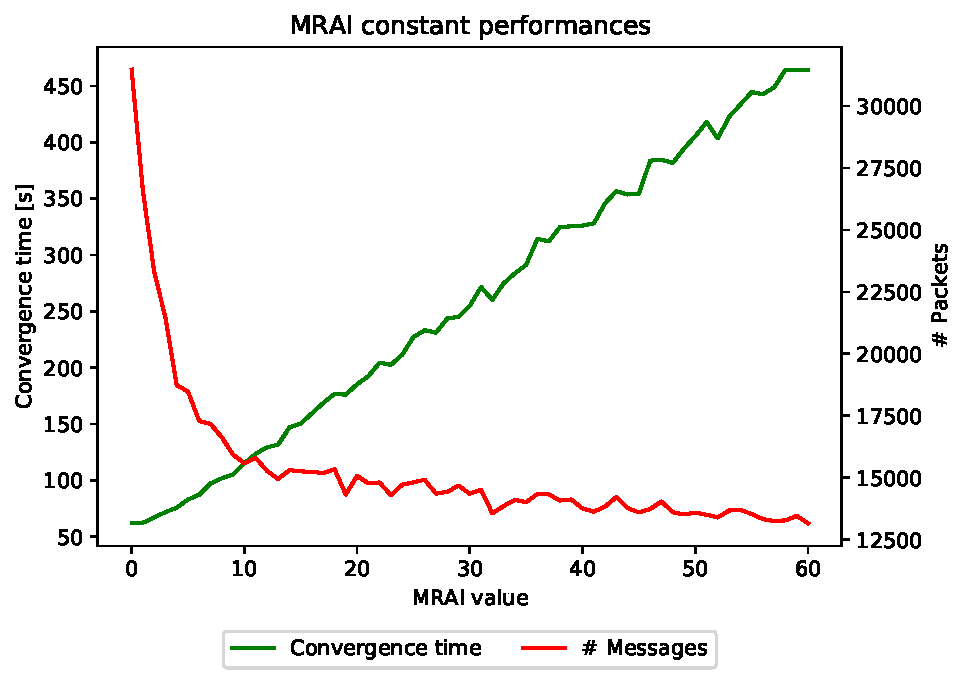
\includegraphics[width=\textwidth]{images/internet_like/1000/constantMRAI/internet_like-constant-noIW_mrai_evolution.pdf}
		 \caption{Network performances, messages VS convergence time with different
			\ac{MRAI} values}
         \label{fig:internt_like_1000_constant_noIW_evolution_evolution}
     \end{subfigure}
     \hfill
     \begin{subfigure}[b]{0.45\textwidth}
         \centering
         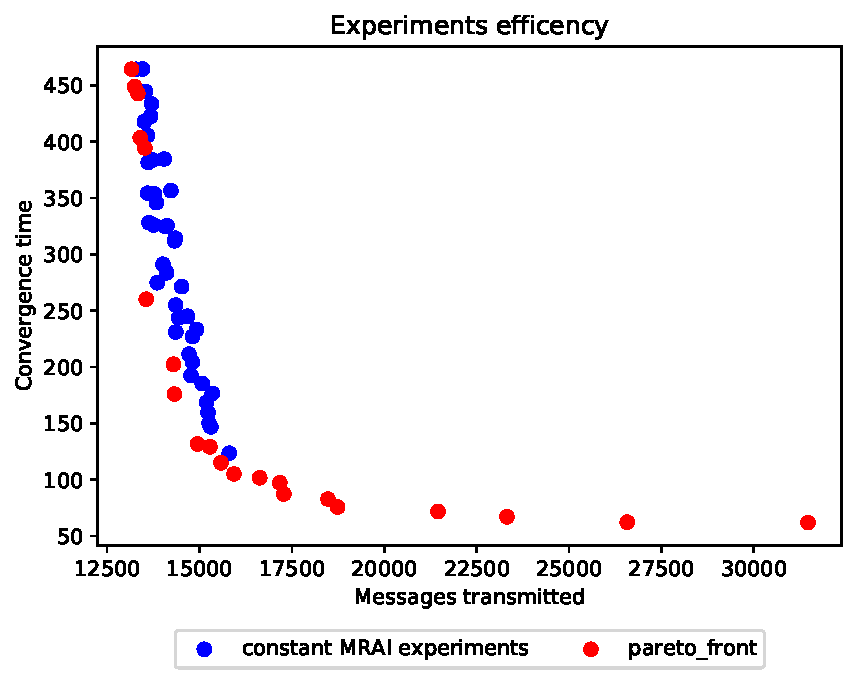
\includegraphics[width=\textwidth]{images/internet_like/1000/constantMRAI/internet_like-constant-noIW.pdf}
		 \caption{Pareto front of Messages VS Convergence time}
         \label{fig:internt_like_1000_constant_noIW_evolution_paretoFront}
     \end{subfigure}
		\caption{Evolution of the network performances on the \textbf{Internet Like} graph 
			of \num{1000} nodes using a fixed \ac{MRAI} from \num{0} to \num{60} seconds.
			\textbf{Without \ac{IW}}}
        \label{fig:internet_like_1000_constant_evolution_noIW}
\end{figure}

Also in this case, comparing \Cref{fig:internet_like_1000_constant_evolution_noIW,fig:internet_like_1000_constant_evolution},
is possible to notice that \ac{IW}
helps to reduce the number of messages and the convergence time without impacting
the network performances trend.

The second strategy, the one dependant on the \ac{DPC}, produced the results
in \Cref{fig:internet_like_1000_dpc_evolution}
As mentioned before, all the timers are adjusted to respect the same mean as in 
the \textit{fixed} \ac{MRAI} experiments.
For this reason points with the same \ac{MRAI} value are comparable to one another.

\begin{figure}[h]
     \centering
     \begin{subfigure}[b]{0.45\textwidth}
         \centering
         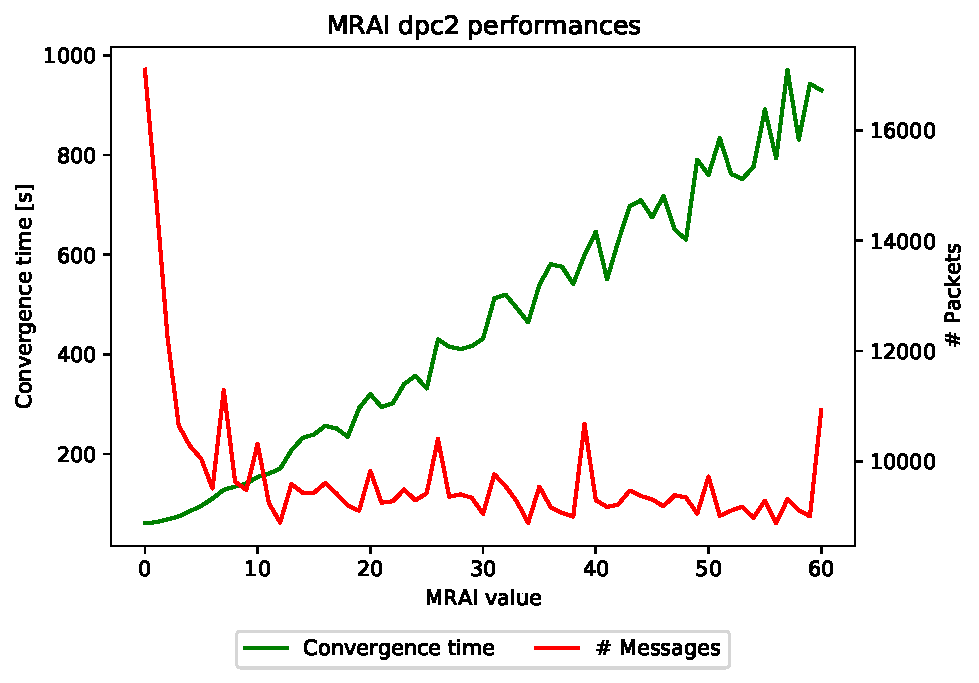
\includegraphics[width=\textwidth]{images/internet_like/1000/dpc/internet_like-DPC_mrai_evolution.pdf}
		 \caption{Network performances, messages VS convergence time with different
			\ac{MRAI} values}
         \label{fig:internt_like_1000_DPC_evolution_evolution}
     \end{subfigure}
     \hfill
     \begin{subfigure}[b]{0.45\textwidth}
         \centering
         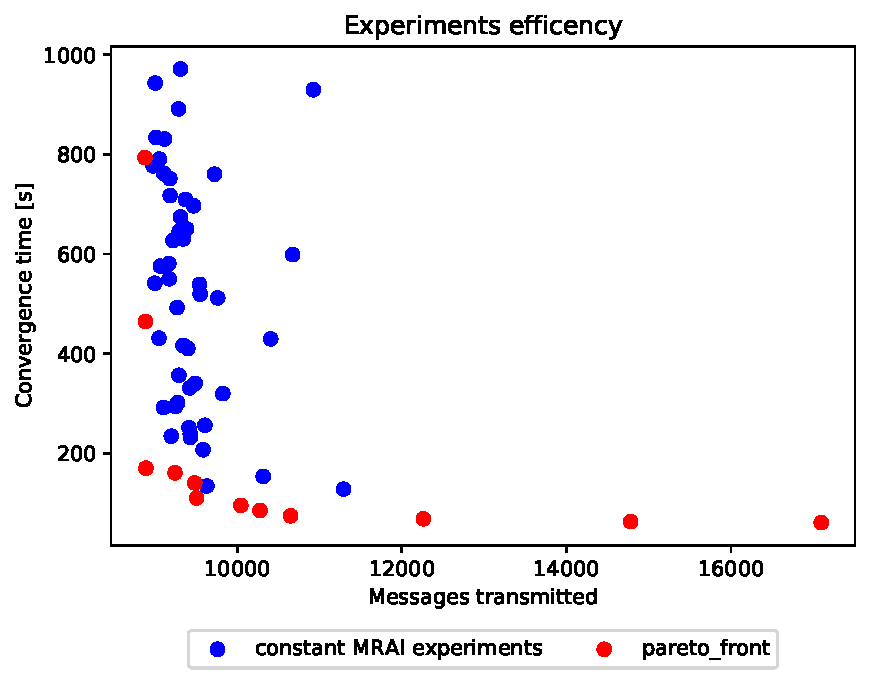
\includegraphics[width=\textwidth]{images/internet_like/1000/dpc/internet_like-DPC.pdf}
		 \caption{Pareto front of Messages VS Convergence time}
         \label{fig:internt_like_1000_DPC_evolution_paretoFront}
     \end{subfigure}
		\caption{Evolution of the network performances on the \textbf{Internet Like} graph 
			of \num{1000} nodes using a \textit{DPC} \ac{MRAI} strategy
			with an $MRAI_{mean}$ from \num{0} to \num{60} seconds.}
        \label{fig:internet_like_1000_dpc_evolution}
\end{figure}

\fxfatal{Cumbersome, reading again it's not very clear what I'm explaining}
This second strategy leads to the performances showed in \Cref{fig:internet_like_1000_dpc_evolution},
is possible to notice that the number of messages transmitted fell down
very quickly and it reaches the convergence value around an \ac{MRAI} value of
\num{10}.
But, it is also noticeable that there are a lot more spikes in this trend, that
deviate more from the constant value around \num{9000} messages.
Also, the convergence time is affected by this behaviour.

\fxfatal{Consider introducing a figure to show both trend in the same plot}
Comparing \Cref{fig:internet_like_1000_dpc_evolution,fig:internet_like_1000_constant_evolution}.

Is possible to notice that the two strategies lead to a different trend.
Both are equal at the beginning with \ac{MRAI} equal \num{0} but, after a while,
both the number of transmitted messages and the convergence time diverge.
The number of messages with the \ac{DPC} strategy variate more and it converges
around \num{9000} messages, while the \textit{fixed} strategy reaches \num{8000}
messages.
And the convergence time with the second strategy grows more quickly.
This is caused by the central clique of tier-one nodes that have a high \ac{MRAI}
value.
The high \ac{MRAI} value is caused by the fact that all the leafs has \num{0.0}
as centrality that cause an \ac{MRAI} value of \num{0} and to respect 
the $MRAI_{mean}$ value the central nodes needs a huge \ac{MRAI}.
For example, with an $MRAI_{mean}$ of \SI{30}{\second} the node \num{1} (that is
one of the central clique nodes) has an \ac{MRAI} value of \num{79.35} for all its
neighbours.


The standard value of \ac{MRAI} is \SI{30}{\second} as described in
\cite{rfc4271} so I compared those strategies performances in a box-plot in 
\Cref{fig:boxplot_internet_like_1000}.
I decided to run \num{100} different runs for each strategy with the $MRAI_{mean}$
fixed to \SI{30}{\second}.

\begin{figure}[h]
     \centering
     \begin{subfigure}[b]{0.45\textwidth}
         \centering
         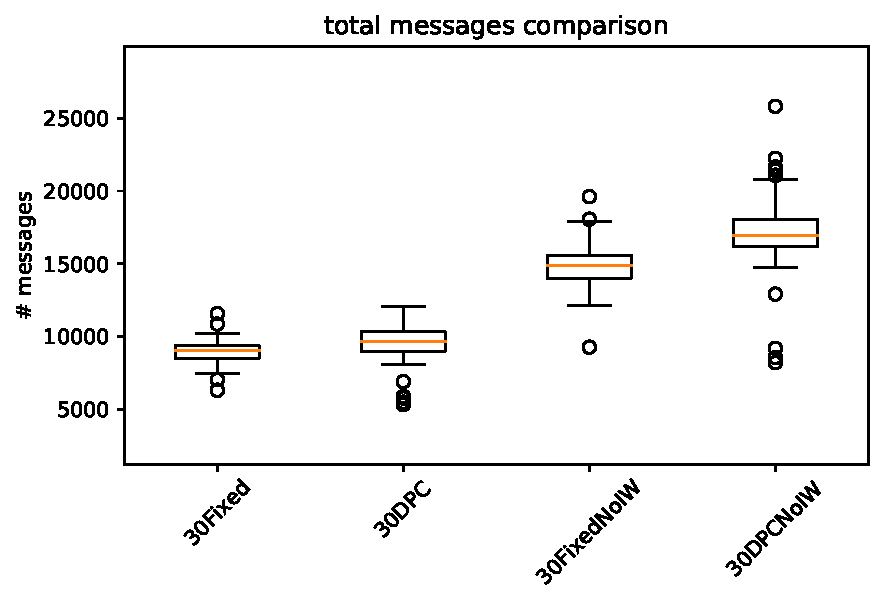
\includegraphics[width=\textwidth]{images/internet_like/1000/comparison/comparison_messages_boxplot.pdf}
		 \caption{Network performances, messages necessary to reach convergence
			with different \ac{MRAI} strategies}
         \label{fig:boxplot_internet_like_1000_messages}
     \end{subfigure}
     \hfill
     \begin{subfigure}[b]{0.45\textwidth}
         \centering
         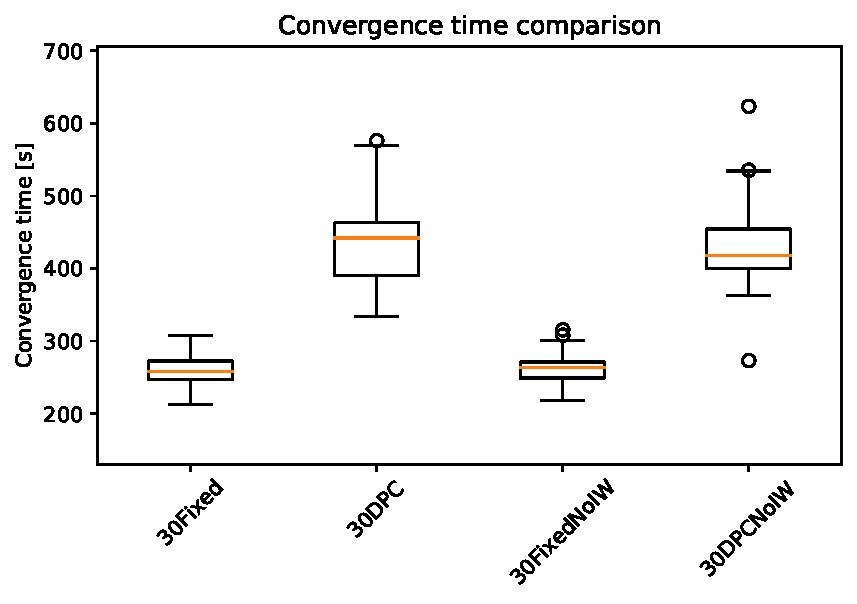
\includegraphics[width=\textwidth]{images/internet_like/1000/comparison/comparison_time_boxplot.pdf}
		 \caption{Network performances, time required to reach convergence
			with different \ac{MRAI} strategies}
         \label{fig:boxplot_internet_like_1000_time}
     \end{subfigure}
	 \caption{Network performances comparison with different \ac{MRAI} strategies,
		Graph internet like with \num{1000} nodes, \ac{MRAI} value 
		\SI{30}{\second}, number of runs for each strategy \num{100}}
        \label{fig:boxplot_internet_like_1000}
\end{figure}

In \Cref{fig:boxplot_internet_like_1000} we can compare those two strategies,
the first figure, \Cref{fig:boxplot_internet_like_1000_messages} represent 
the number of messages transmitted by the \num{100} runs, we can see that
the two strategies, without \ac{IW}, are really close to one another.
While in the time required for convergence, \Cref{fig:boxplot_internet_like_1000_time}
there are some huge difference between the two strategies, is not negligible 
that with the \ac{DPC} strategy the time required is almost the double of the
standard time.

In conclusion, we can say that the \ac{MRAI} strategy is one of the factors that 
can influence the Network performances. 

\fxfatal{Maybe I can introduce more strategies to expand this section}

\section{Pareto Efficiency Front}
\label{sec:bgp_mrai_pareto_front}

The strategies exposed in \Cref{sec:bgp_mrai_strategy_dependance} are just few
of the possibilities that are available.
For this reason, I would like to explore the set of possibilities looking 
for \ac{MRAI} configuration randomly generated.

I would then study the space of possibilities that are generated through the 
Pareto efficiency plot and compare the results with the Pareto efficiency
graphs.
To permit this comparison I would set \ac{MRAI} randomly but like for
the \ac{DPC} strategy respecting the average required.

The environemnt used for those experiments is showed in \Cref{tbl:random_env}

\begin{table}[h]
	\begin{center}
	\begin{tabular}{ || m{4.9cm}| m{7.3cm} || } 
	\hline
	Property & Value \\ 
	\hline \hline
	Seeds & $[1, 10]$ \\ 
	\hline
	Signaling & \q{AW} \\
	\hline
		Withdraws delay & Uniform distribution between \SI{1}{\second} and \SI{60}{\second} \\ 
	\hline
		Implicit withdraw & Active \\ 
	\hline
		MRAI mean & $[0, 60]$ \\
	\hline
		MRAI values & Uniform distribution between \SI{1}{\second} and \SI{120}{\second} \\
	\hline
		Experiments per \ac{MRAI} mean & \num{10} \\
	\hline
	Link delay & Uniform distribution between \SI{0.012}{\second} and \SI{3}{\second} \\
	\hline

	\end{tabular}
\end{center}

	\caption{Random \ac{MRAI} environment properties}
	\label{tbl:random_env}
\end{table}

Thanks to this environment I'm going to run in total more than \num{600} compleate
experiments.
For each \ac{MRAI} mean value I will generate \num{10} different graph with a random
assignment of \ac{MRAI} for each link.
I wil then execute \num{10} different runs for each radom graph that will produce
the average result of \num{1} experiment.
The total number of experiments is \num{610}.

in \Cref{fig:random_pareto_front} is possible to see all the \num{601} points
generated.

\begin{figure}[h]
    \centering
    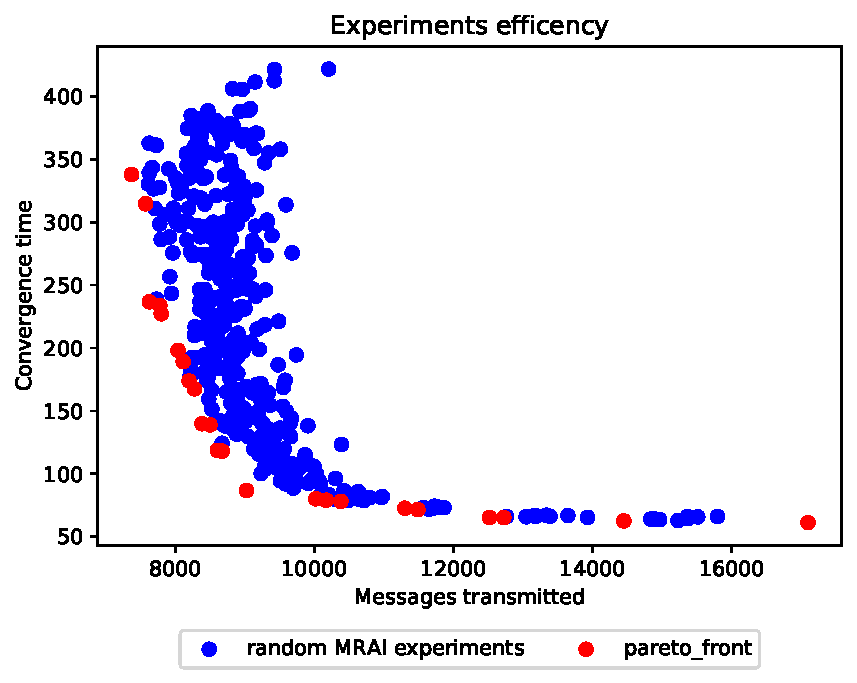
\includegraphics[width=.5\textwidth]{images/internet_like/1000/random.pdf}
	\caption{Pareto front generated by \num{601} experiments on an internet like
	topology with \num{1000} nodes, \ac{MRAI} generted randomly and adapted to 
	the mean}
    \label{fig:random_pareto_front}
\end{figure}

As we can see the trend in \Cref{fig:random_pareto_front} is similar to the one
that we saw for the same signal in \Cref{sec:bgp_mrai_strategy_dependance}.
For the majority of configuration the number of messages transmitted is never
over \num{10000} but the time required to converge grows continuously.

In \Cref{fig:pareto_comparison} is present a comparison between the random
experiments, the fixed \ac{MRAI} strategy and the \ac{DPC} strategy from
\Cref{fig:internet_like_1000_constant_evolution_paretoFront,fig:internt_like_1000_DPC_evolution_paretoFront}

\begin{figure}[h]
    \centering
    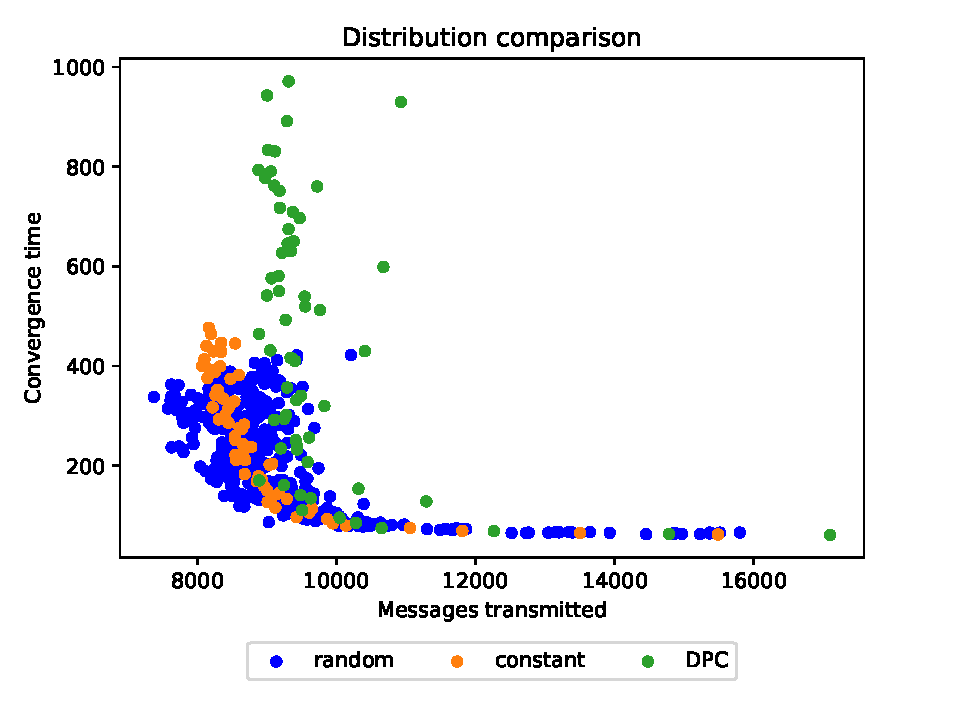
\includegraphics[width=.5\textwidth]{images/internet_like/1000/random_vs_all.pdf}
	\caption{Pareto front generated by \num{601} experiments on an internet like
	topology with \num{1000} nodes, \ac{MRAI} generted randomly and adapted to 
	the mean, vs fixed \ac{MRAI} strategy and \ac{DPC} \ac{MRAI} strategy.}
    \label{fig:pareto_comparison}
\end{figure}

As we can see in \Cref{fig:pareto_comparison} all the strategies have the same
behaviour, but is also possible to see that the random strategy is the only
one with experiments that produces less than \num{8000} messages.
This is important because it a prove that there are better possibilities rather
that the classical one.

For this reason \ac{MRAI} can be tuned to have a better trade-off between 
number of messages transmitted and convergence time.

\section{Signal dependence}
\label{sec:bgp_mrai_signal_dependance}

I would like to analyze how much the signal can impact the convergence performances
with the two different strategies of \Cref{sec:bgp_mrai_strategy_dependance}.

For this reason, I used the same environment described before and execute the
experiments with different input signals from the same node, \q{AWA}, \q{AWAW}
and \q{AWAWA}.

In those experiments plays a role also the \q{\textit{re-advertisement distribution}}
for the second and third \q{A}, it has been set to a uniform distribution
between \SI{1}{\second} and \SI{60}{\second}, like the \q{\textit{withdraw distribution}}.

For those experiments, I didn't evaluate the case with \ac{IW} deactivated.
\fxfatal{Explain why}

\fxfatal{all the plots has an \ac{MRAI} steep of \SI{10}{\second} to give a 
hint on the trend, redo the plots with a step of \SI{1}{\second}}

In \Cref{fig:internt_like_1000_evolution_AWA} is possible to see the evolution
for the signal \q{AWA}.

\begin{figure}[h]
     \centering
     \begin{subfigure}[b]{0.45\textwidth}
         \centering
         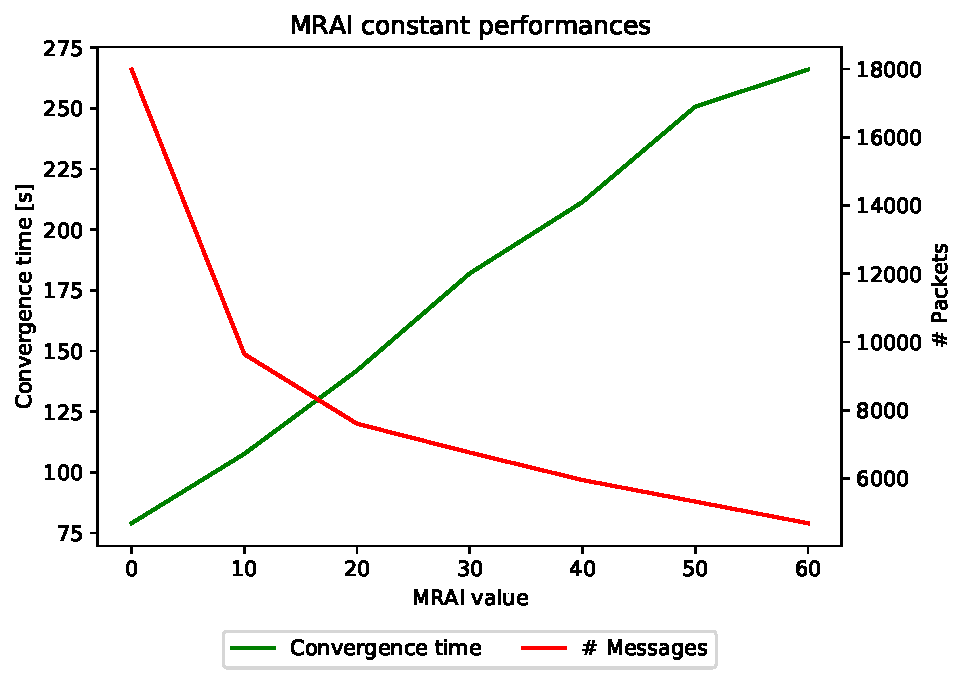
\includegraphics[width=\textwidth]{images/internet_like/1000/signals/AWA/constant/internet_like-constant_AWA_mrai_evolution.pdf}
		 \caption{Network performances, \textit{fixed} \ac{MRAI} strategy}
         \label{fig:internet_like_1000_fixed_AWA}
     \end{subfigure}
     \hfill
     \begin{subfigure}[b]{0.45\textwidth}
         \centering
         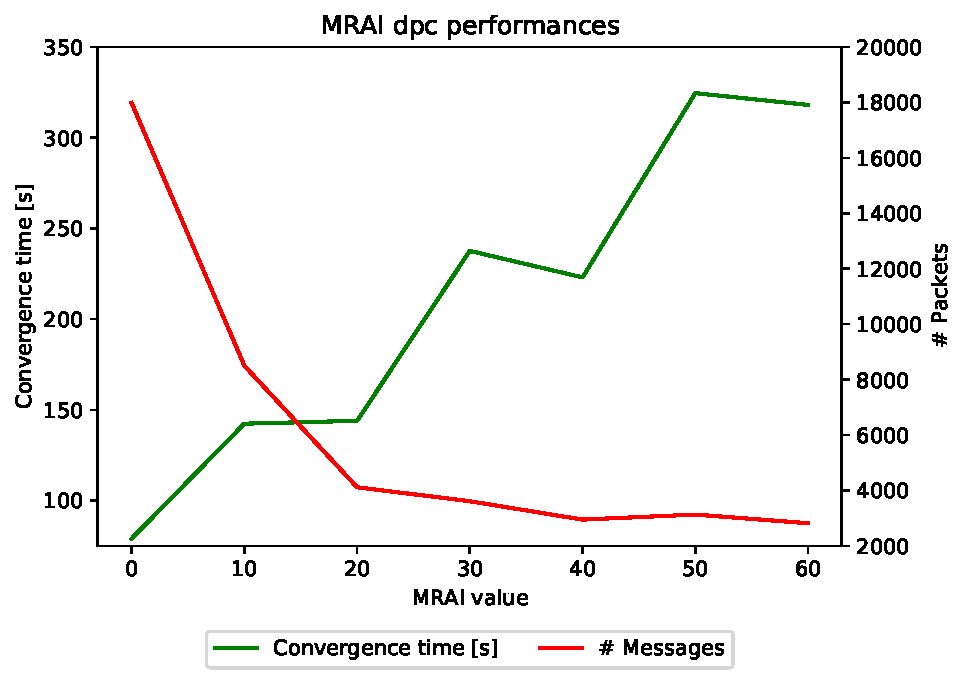
\includegraphics[width=\textwidth]{images/internet_like/1000/signals/AWA/dpc/internet_like-DPC_AWA_mrai_evolution.pdf}
		 \caption{Network performances, \ac{DPC} \ac{MRAI} strategy}
         \label{fig:internet_like_1000_dpc_AWA}
     \end{subfigure}
	 \caption{Network performances comparison with different \ac{MRAI} strategies,
		Graph internet like with \num{1000} nodes, signal \q{AWA}}
        \label{fig:internt_like_1000_evolution_AWA}
\end{figure}

Is possible to notice in \Cref{fig:internt_like_1000_evolution_AWA} a huge difference
in respect of the plots in \Cref{fig:internet_like_1000_constant_evolution,fig:internet_like_1000_dpc_evolution}.
The \ac{DPC} strategy was able to outcome the standard \textit{fixed} strategy
over multiple prospective.
Analyzing \Cref{fig:internet_like_1000_dpc_AWA} is possible to notice that
the red curve, the one that refers to the number of messages transmitted has
a very fast fell, with an average \ac{MRAI} timer \textit{of \SI{30}{\second}}
the number of messages is less than $1/4$ in respect of an \ac{MRAI} \textit{mean}
of \SI{0}{\second}.
The convergence time curve has a completely different trend in respect of the
previous experiments.
We can notice some steps trend.
This is caused by the fact that now the timer is able to effectively act on the signal.
\ac{MRAI} doesn't affect the first message, in this case the first \q{A} of the
signal, but it can affect the next two messages.
In fact, some nodes are able to cache both the \q{WA} part of the signal and
completely avoid sending anything at all, because they have already transmitted
the first \q{A}.
The complete compression of the signal \q{AWA} is \q{A}.
The other evolution, for the \q{AWAW} and \q{AWAWA} signals, are showed in 
\Cref{fig:internt_like_1000_evolution_AWAW,fig:internt_like_1000_evolution_AWAWA}

Like before, comparing the standard \SI{30}{\second} fixed \ac{MRAI} I executed
\num{100} different runs for each strategy and each different signal, the results
are exposed in \Cref{fig:boxplot_internet_like_1000_time_allSignals}.

\begin{figure}[h]
     \centering
     \begin{subfigure}[b]{0.45\textwidth}
         \centering
         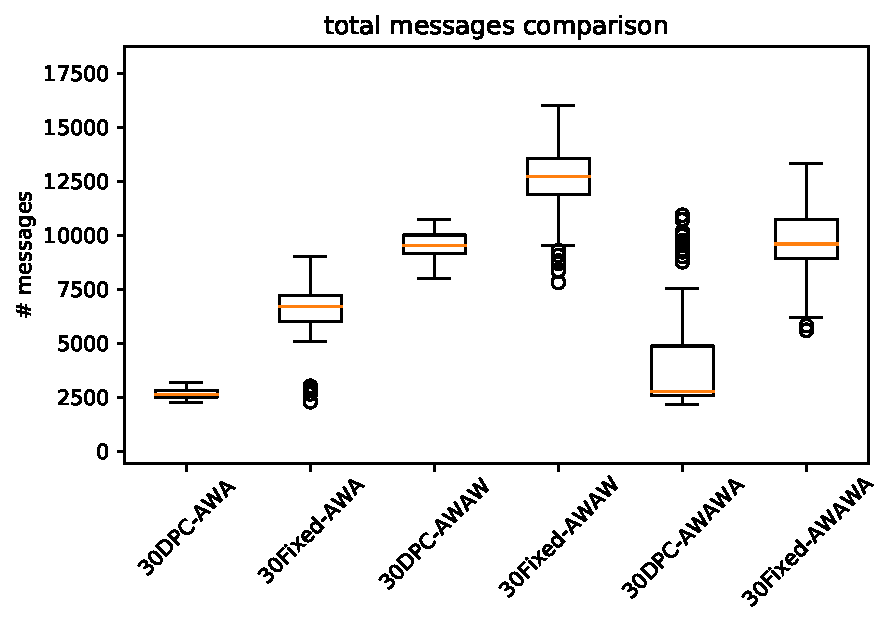
\includegraphics[width=\textwidth]{images/internet_like/1000/comparison/comparison_allSignals_messages_boxplot.pdf}
		 \caption{Network performances, messages necessary to reach convergence
			with different \ac{MRAI} strategies}
         \label{fig:boxplot_internet_like_1000_messages_allSignals}
     \end{subfigure}
     \hfill
     \begin{subfigure}[b]{0.45\textwidth}
         \centering
         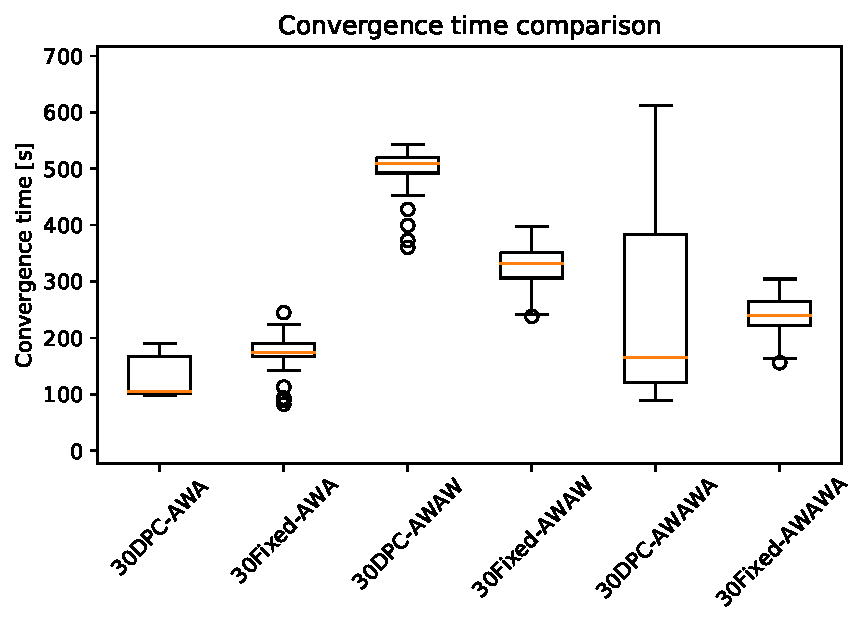
\includegraphics[width=\textwidth]{images/internet_like/1000/comparison/comparison_allSignals_time_boxplot.pdf}
		 \caption{Network performances, time required to reach convergence
			with different \ac{MRAI} strategies}
         \label{fig:boxplot_internet_like_1000_time_allSignals}
     \end{subfigure}
	 \caption{Network performances comparison with different \ac{MRAI} strategies,
		Graph internet like with \num{1000} nodes, \ac{MRAI} value 
		\SI{30}{\second}, number of runs for each strategy \num{100}, signal \q{allSignals}}
        \label{fig:boxplot_internet_like_1000_allSignals}
\end{figure}

Is possible to notice in \Cref{fig:boxplot_internet_like_1000_allSignals} that
both the strategies have different performances in respect of the signal 
produced by the single node source.
In particular, performances are better when the signal ends up with an \q{A}.
That's because, after the first \q{A}, giving the \ac{MRAI} timer long enough, 
a node is able to compress a sequence that ends with another \q{A} to the
empty set and don't send anything more.
While if the sequence ends up with an \q{W} it has to, at least, send another
message to notify the withdraw.
%And withdraws are not affected by \ac{MRAI} like specified in a IETF draft of
%\num{2012} named \q{Revisions to the BGP 'Minimum Route Advertisement Interval'}.

Other than that is possible to notice that the \ac{DPC} techniques has better
results in terms of messages transmitted, while it could have a higher 
convergence time.
This is caused like before by the high \ac{MRAI} values used by the most
central nodes.

In conclusion, there is a correlation between \ac{MRAI} and the sequence of messages
transmitted by the source node.
In particular more the timer is able to compress sequence more the performances
are good.

\fxfatal{consider moving figures from the appendix to the chapter}

\section{Position dependence}
\label{sec:position_dependance}

The last factor of influence for \ac{MRAI} that I would like to study is how much
the position of the signal source can influence the convergence.
The main hypothesis is that a node closer to the central clique, that generates
a signal would provoke a message storm bigger in respect of a node on the perimeter
of the network.
This is true only if \ac{MRAI} is large enough to block the storm near the source
of it exporting only the correct information at the end of it.

\subsection{Different signal sources}
\label{subsec:different_destinations}

As first try I have decided to try \num{10} different destination chosen randomly
on the same graph, this graph is an Internet like topology with \num{1000} nodes.
After that, I run the same environment with all the different destination.
I also used different \ac{MRAI} strategies, repeating the experiments for all of
them.
With this results is possible to analyze how different signal sources provoke 
different network performances and also study how different \ac{MRAI} strategies
adapt to different nodes that provoke messages storms.

The environemnt used by those experiments is the one described in 
\Cref{tbl:source_properties}.

\begin{table}[h]
	\begin{center}
	\begin{tabular}{ || m{4cm}| m{8cm} || }
	\hline
	Property & Value \\
	\hline \hline
	Seeds & $[1, 10]$ \\
	\hline
	Signaling & \q{AWAWA} \\
	\hline
		Withdraws delay & Uniform distribution between \SI{0.1}{\second} and \SI{60}{\second} \\
	\hline
	Announcement delay & Uniform distribution between \SI{0.1}{\second} and \SI{60}{\second} \\
	\hline
	Link delay & Uniform distribution between \SI{0.0001}{\second} and \SI{0.5}{\second} \\
	\hline
			\(MRAI_{mean}\) & $[0, 60]$ with steps of \num{10} \\
	\hline
		Random nodes & \num{10} \\
	\hline
		\ac{MRAI} strategies & Fixed \ac{MRAI}, \ac{DPC}, reverse \ac{DPC} \\
	\hline
	\end{tabular}
\end{center}

	\caption{Different signal sources environment properties}
	\label{tbl:source_properties}
\end{table}

Like mentioned in \Cref{tbl:source_properties} I decided to use an other 
\ac{MRAI} strategy and look forward for it performances.
That strategy is the reverse of the one base on the \ac{DPC}.
I will use a higher \ac{MRAI} for the first part of the graph and a smaller 
one in the propagation part of the graph.

In total I have executed \num{700} runs for each \ac{MRAI} strategy with the 
\num{10} different signal sources.
The resulting network evolution with different \ac{MRAI} values is showed in 
\Cref{fig:different_destinations}.
Each point of \Cref{fig:different_destinations_all} represents the average 
of the \num{10} runs executed for the specific destination with that \ac{MRAI}
configuration.
On \Cref{fig:different_destinations_mean} is presented the average result
obtained from all the \num{10} different destinations for a specific \ac{MRAI}
strategy.

\begin{figure}[h]
     \centering
     \begin{subfigure}[b]{0.45\textwidth}
         \centering
         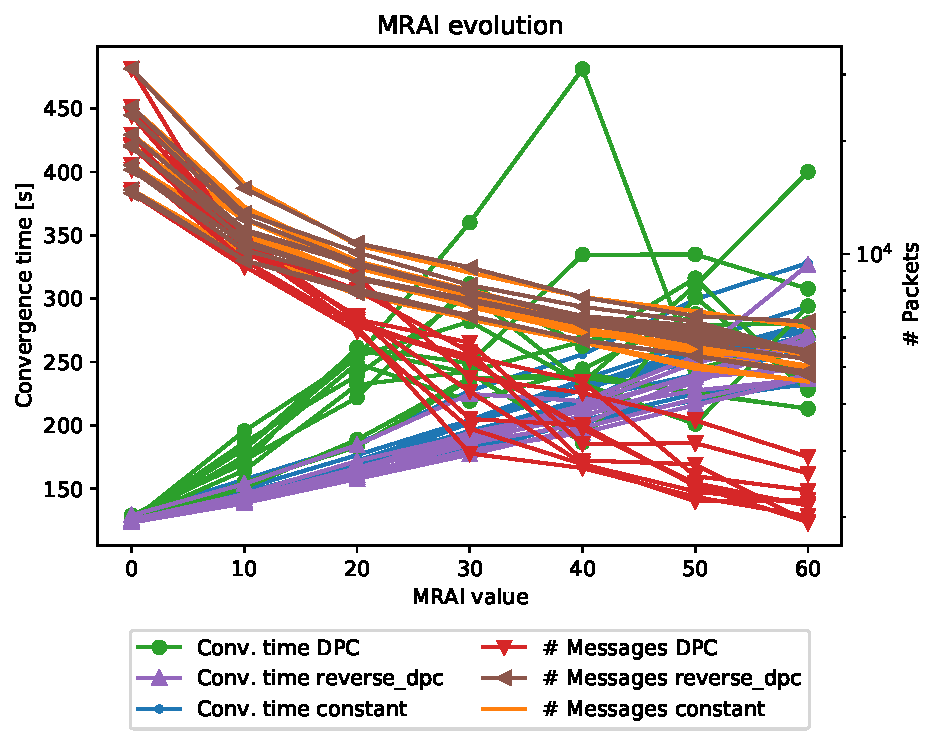
\includegraphics[width=\textwidth]{images/position/different_destinations-1000_all.pdf}
		 \caption{Network performance evolution of all the \num{10} different signal sources 
			with the different \ac{MRAI} strategies}
         \label{fig:different_destinations_all}
     \end{subfigure}
     \hfill
     \begin{subfigure}[b]{0.45\textwidth}
         \centering
         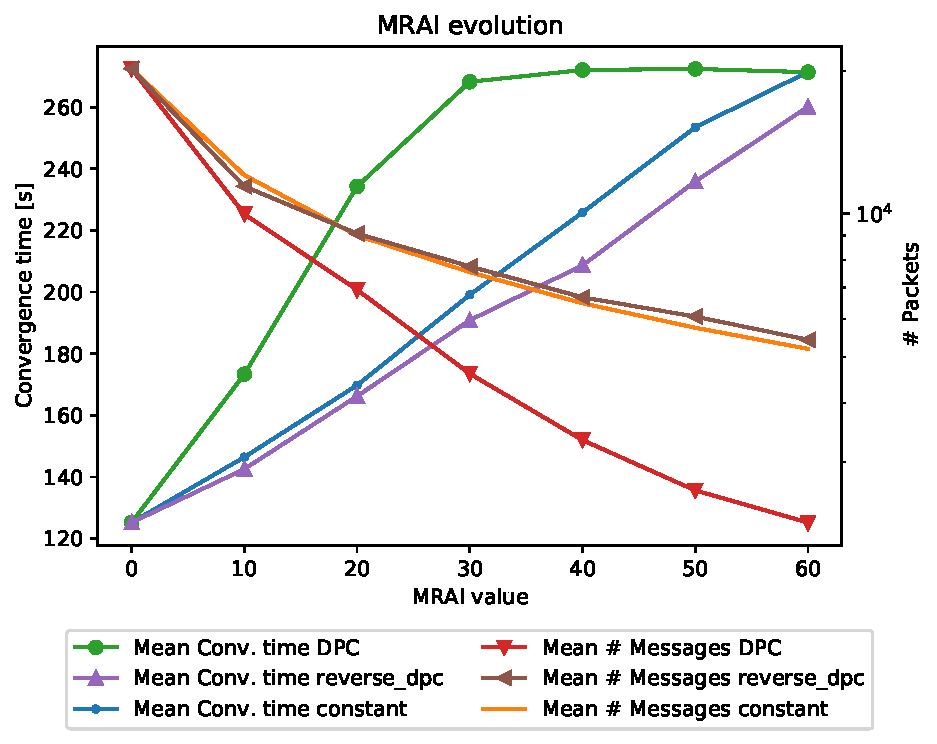
\includegraphics[width=\textwidth]{images/position/different_destinations-1000_mean.pdf}
		 \caption{Average of the network performances of \num{10} different 
			signal sources chosen with different \ac{MRAI} strategies}
         \label{fig:different_destinations_mean}
     \end{subfigure}
	 \caption{Network performances given \num{10} different signal sources chosen
		randomly on an Internet like graph of \num{1000} nodes, with different
		\ac{MRAI} strategies used, fixed, \ac{DPC}, Reverse \ac{DPC}, and 
		different \ac{MRAI} mean values}
	 \label{fig:different_destinations}
\end{figure}

\Cref{fig:different_destinations} shows how, changing the soruce of the signal,
also changes the network performances with multiple \ac{MRAI} values.
Notice that the second y-axis, the one that represents the number of packets
transmitted, is in log scale.
We can use the plot in \Cref{fig:different_destinations_all} to see the 
differences between one destination and the others, while \Cref{fig:different_destinations_mean}
expose the differences between different strategies.
We can see in \Cref{fig:different_destinations_all} that all the \num{10} destinations
causes a similar behaviour with the fixed strategy and the reverse \ac{DPC}, both
in terms of messages transmitted and also convergence time.
In both techniques the difference between the \num{10} destinations in terms of
convergece time is few tens of seconds, with a linear growth.
Thanks to \Cref{fig:different_destinations_mean} is possible to see that the
number of messages reaches a convergence value around between \num{5000} and
\num{6000}.
The \ac{DPC} strategy seems to bee more volatile with the growth of \ac{MRAI}
both in terms of messages and also convergence time.
We can clearly see from multiple green spikes in \Cref{fig:different_destinations_all}
that the position of the source is highly affective using this strategy.

\fxfatal{Consider using a table to show the average and the std var of conv time
and messages}

We can conclude that the position of the source can influence the behaviour
of \ac{MRAI}, its most influente when the strategy used relies on topological
information, like the \ac{DPC} strategy.

\subsection{Hierarchical influence}
\label{subsec:hierarchical_influence}

What about the position in the hierarchy?
Internet is very strong hierarchical graph, \Cref{fig:internet_graph_hierarchical}
is an example with a small set of nodes but it is possible to define different levels
of the graph.
If we take the central clique as the root of the graph then all the nodes will
be at a certain distance (in terms of hops) from it.

Nodes that are on the same hierarchical level reacts in the same way? 

To analyze this possibility I decided to take \num{3} node randomly from each
hierarchical level of an Internet-like graph of \num{1000} nodes, the number
of levels on this graph was \num{4}.
The total number of destinations was \num{12} and for each one of them I executed
an experiment with multiple \ac{MRAI} strategies and multiple possible \ac{MRAI}
values.

The properties of this environment are summarized in \Cref{tbl:hierarchical_properties}.

\begin{table}[h]
	\begin{center}
	\begin{tabular}{ || m{4cm}| m{8cm} || } 
	\hline
	Property & Value \\ 
	\hline \hline
	Seeds & $[1, 10]$ \\ 
	\hline
	Signaling & \q{AWAWAWAW} \\
	\hline
		Withdraws delay & Uniform distribution between \SI{0.1}{\second} and \SI{5}{\second} \\ 
	\hline
	Announcement delay & Uniform distribution between \SI{0.1}{\second} and \SI{5}{\second} \\ 
	\hline
	Link delay & Uniform distribution between \SI{0.0001}{\second} and \SI{0.5}{\second} \\
	\hline
		MRAI & $[0, 60]$ with steps of \num{10} \\
	\hline
		Number of levels & \num{4} \\
	\hline
		Random dst per level & \num{3} \\
	\hline
		\ac{MRAI} strategies & \ac{DPC}, reverse \ac{DPC} \\
	\hline
	\end{tabular}
\end{center}

	\caption{Hierarchical experiments environment properties}
	\label{tbl:hierarchical_properties}
\end{table}

Given that we are evaluating the impact of nodes by their distance from 
the center of the network, it could be a good way also to test strategies
which goal is to enforce those points, for this reason I chose those two
strategies.

The results in \Cref{fig:different_levels} shows the different evolution of
the random source for each different level, from the first to the fourth.

\begin{figure}[h]
     \centering
     \begin{subfigure}[b]{0.45\textwidth}
         \centering
         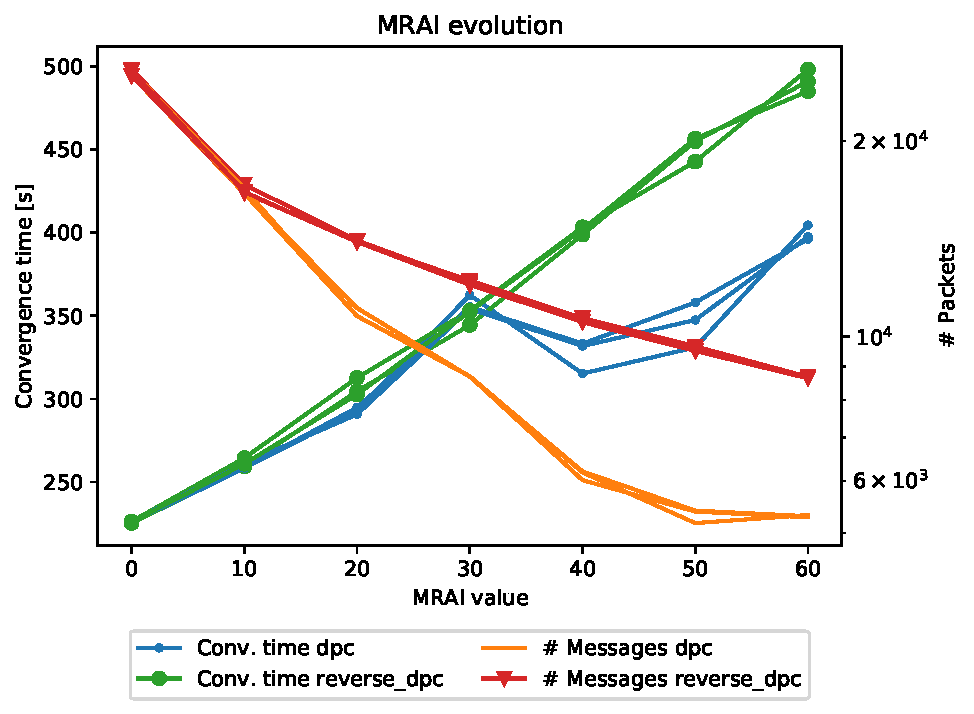
\includegraphics[width=\textwidth]{images/hierarchy/different_levels-1000_hier_1_all.pdf}
		 \caption{Network performances evolution of all the \num{3} different signal sources 
			with the different \ac{MRAI} strategies at the hierarchical level \num{1}}
         \label{fig:different_levels_1}
     \end{subfigure}
     \begin{subfigure}[b]{0.45\textwidth}
         \centering
         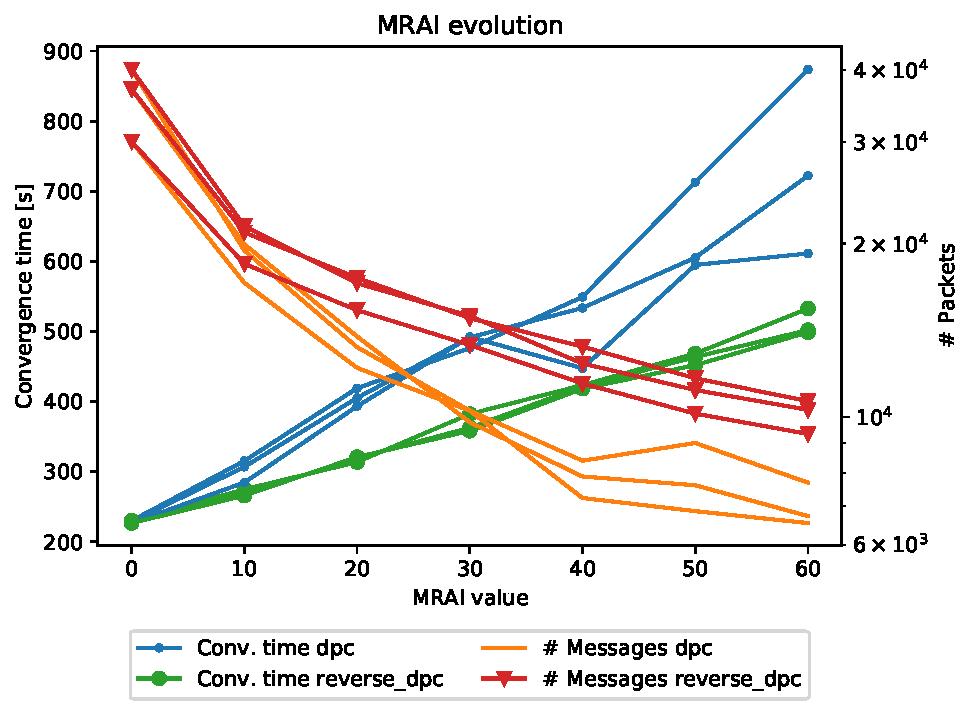
\includegraphics[width=\textwidth]{images/hierarchy/different_levels-1000_hier_2_all.pdf}
		 \caption{Network performances evolution of all the \num{3} different signal sources 
			with the different \ac{MRAI} strategies at the hierarchical level \num{2}}
         \label{fig:different_levels_2}
     \end{subfigure}
     \begin{subfigure}[b]{0.45\textwidth}
         \centering
         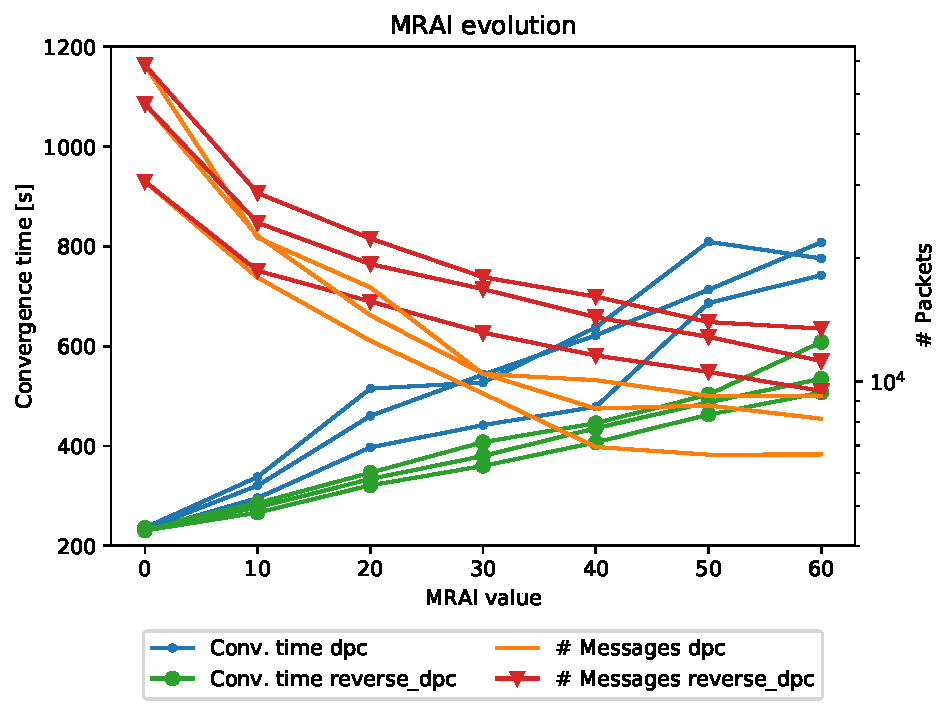
\includegraphics[width=\textwidth]{images/hierarchy/different_levels-1000_hier_3_all.pdf}
		 \caption{Network performances evolution of all the \num{3} different signal sources 
			with the different \ac{MRAI} strategies at the hierarchical level \num{3}}
         \label{fig:different_levels_3}
     \end{subfigure}
     \begin{subfigure}[b]{0.45\textwidth}
         \centering
         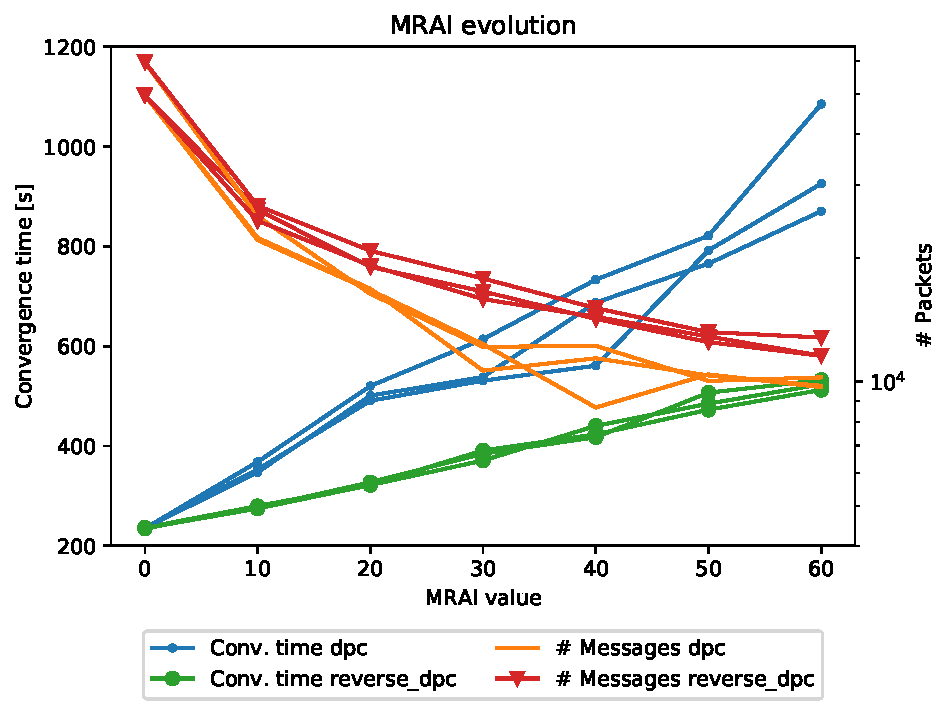
\includegraphics[width=\textwidth]{images/hierarchy/different_levels-1000_hier_4_all.pdf}
		 \caption{Network performances evolution of all the \num{3} different signal sources 
			with the different \ac{MRAI} strategies at the hierarchical level \num{4}}
         \label{fig:different_levels_4}
     \end{subfigure}
     \hfill
	 \caption{Network performances given \num{3} different signal sources chosen
		randomly for each level of the Internet like graph, number of nodes 
		\num{1000}, number of levels \num{4}, different \ac{MRAI} strategies
		\ac{DPC} and reverse \ac{DPC} \fxfatal{figures don't have the same
		y-axis}}
	 \label{fig:different_levels}
\end{figure}

In \Cref{fig:different_levels} is possible to see the evolution of the network
with different source nodes from different levels and how \ac{MRAI} influence
the network performances.
Starting from the first level in \Cref{fig:different_levels_1}, where the source
node was directly connected with a node of the central clique we can see different
important things.
First of all, the varaince that the three different sources has is very small, 
both in terms of messages transmitted and also convergence time.
Both the techniques, \ac{DPC} and the reverse of it, in terms of messages
transmitted starts from a value around \num{25000} whit \ac{MRAI} equal to 
\SI{0}{\second} and both reaches a value under \num{10000} units.
In terms of convergence time the reverse strategy grows linearly as expected
while the \ac{DPC} technique is able to gain a strong reduction thanks to
the efficient messages compression.
Going to the second and third level, respectively in 
\Cref{fig:different_levels_2,fig:different_levels_3} when can see thtat there
is an increase of the varaince between the single source trends, both in terms
of messages and also convergence time.
Also, the number of messages transmitted slowly increases, at the beginning the 
number of messages reaches \num{60000} units converging around \num{10000}.
In \Cref{fig:different_levels_3} we can see the worst case scenario, not in 
terms of varaiance between the sources, but in this case we have the worst
performances.
The convergence time grows even over \SI{1000}{\second} for the \ac{DPC} strategy.
While the number of messages transmitted with \ac{MRAI} equal to \SI{0}{\second}
touches \num{60000} reaching a convergence value slightly over \num{10000}.

We can clearly see the influence that the position of the source nodes has to
a hierarchical graph like Internet.
The performances with \ac{MRAI} at \SI{0}{\second} are only atribuible to the
strategic position of the source node.

An other hypothesis is that there is a difference in the single nodes based
on the position in the topology.
Nodes that are more central, if the signal comes from closer nodes could
react with a more explosive \textit{Path exploration} behaviour.
If the signal comes from the periphery of the network, the other side of
it could require more time to converge in respect of a signal that starts 
near the center.

To prove those hypotesis I decided to use the data from this set of experiments
with \ac{MRAI} value equal to \SI{30}{\second}.
I calculated for each node the average performances, based on the level, convergence
time, number of messages necessary to reach the convergence state and \ac{DPC}
centrality value (that is dependant on the position of the source).
I have then grouped nodes that are at the same distance from the source, to 
calculate the distance I used the distance in terms of hops in the \textit{Best
Path}.
I then calculated the average performances of each group.
The results are showed in \Cref{fig:different_levels_comparison}.

\begin{figure}[h]
     \centering
     \begin{subfigure}[b]{0.45\textwidth}
         \centering
         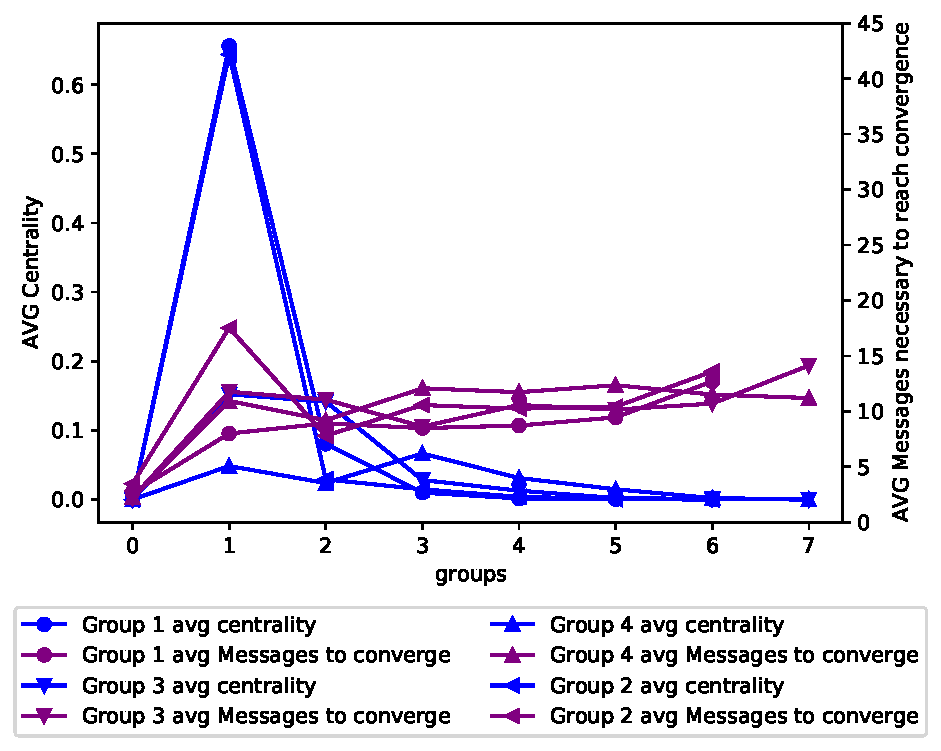
\includegraphics[width=\textwidth]{images/hierarchy/dpc_all_levels_comparison_centVSmsg.pdf}
		 \caption{\ac{MRAI} strategy \ac{DPC}, number of messages necessary on
			average to reach convergence, levels comparison}
         \label{fig:different_levels_comparison_dpc_msg}
     \end{subfigure}
     \begin{subfigure}[b]{0.45\textwidth}
         \centering
         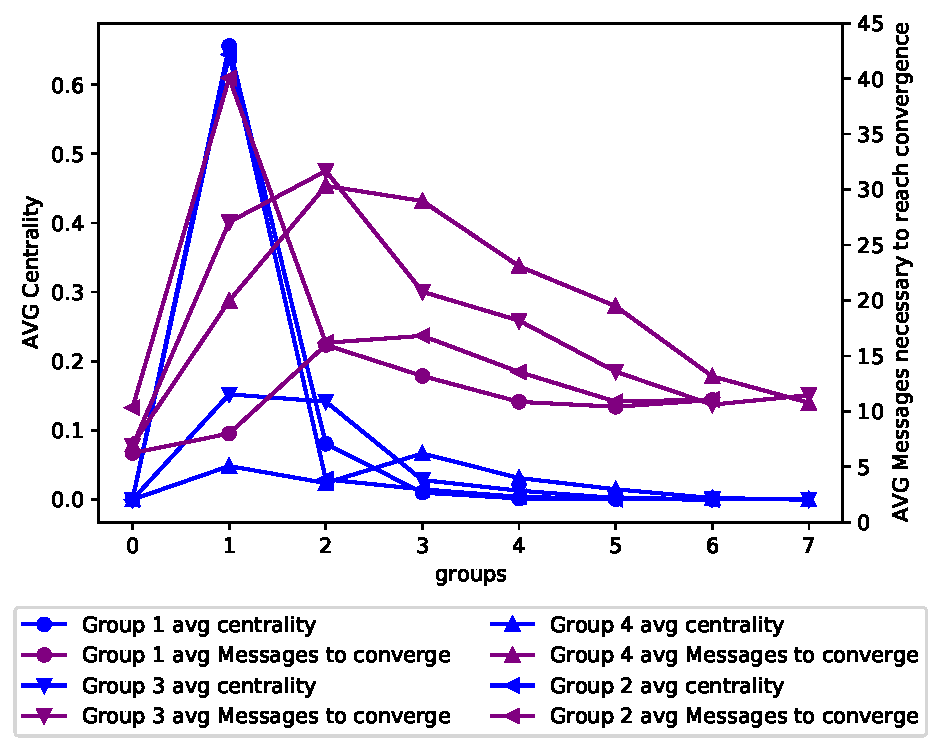
\includegraphics[width=\textwidth]{images/hierarchy/reverse_dpc_all_levels_comparison_centVSmsg.pdf}
		 \caption{\ac{MRAI} strategy reverse \ac{DPC}, number of messages necessary on
			average to reach convergence, levels comparison}
         \label{fig:different_levels_comparison_reverse_dpc_msg}
     \end{subfigure}
     \begin{subfigure}[b]{0.45\textwidth}
         \centering
         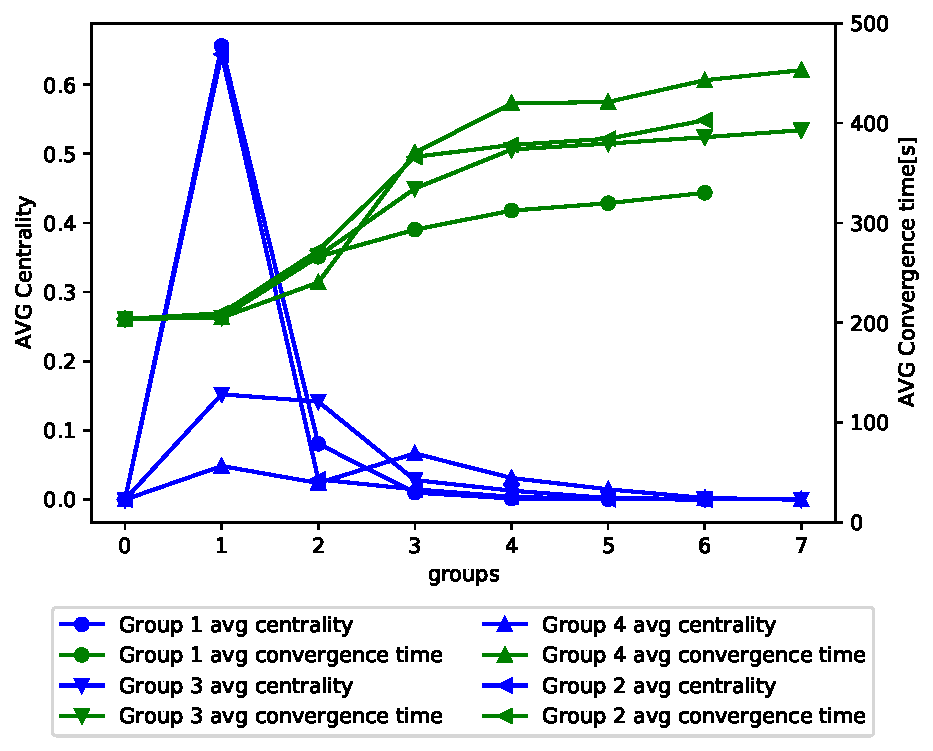
\includegraphics[width=\textwidth]{images/hierarchy/dpc_all_levels_comparison_centVStime.pdf}
		 \caption{\ac{MRAI} strategy \ac{DPC}, convergece time levels comparison}
         \label{fig:different_levels_comparison_dpc_time}
     \end{subfigure}
     \begin{subfigure}[b]{0.45\textwidth}
         \centering
         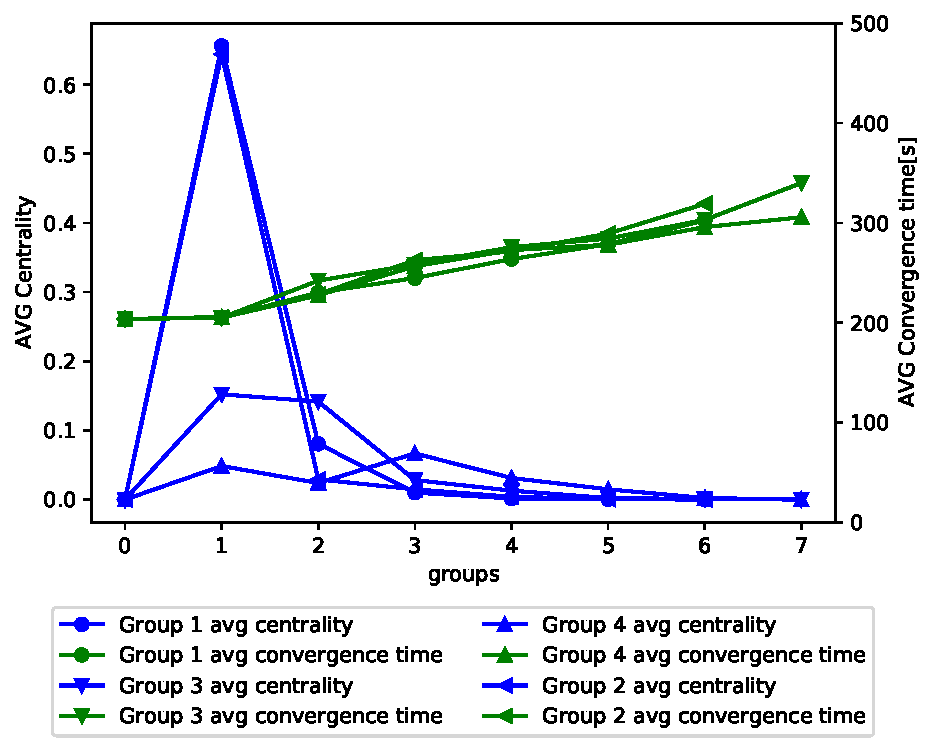
\includegraphics[width=\textwidth]{images/hierarchy/reverse_dpc_all_levels_comparison_centVStime.pdf}
		 \caption{\ac{MRAI} strategy reverse \ac{DPC}, convergece time levels comparison}
         \label{fig:different_levels_comparison_reverse_dpc_time}
     \end{subfigure}
     \hfill
	 \caption{Internet like topology of \num{1000} nodes grouped by the distance
	 from the signal source, different level comparison with \ac{MRAI} strategy
	 \ac{DPC} and reverse \ac{DPC}, \ac{MRAI} value equal to \SI{30}{\second}
	 \fxfatal{Maybe could be more interesting to see how \ac{DPC} vs \texit{Fixed}
	 goes}, \fxfatal{I think this is the wrong way to show the AVG centrality, it
	 depends on the position of the source, for the same level i cant AVG it}}
	 \label{fig:different_levels_comparison}
\end{figure}

In \Cref{fig:different_levels_comparison} is possible to see an anlysis of the
average nodes performanes grouped by the distance from the source of the signal.
Those performances are taken from the case where \ac{MRAI} is equal to
\SI{0}{\second}.
On the left side, is possible to see the performances of the nodes that uses the
\ac{DPC} \ac{MRAI} strategy, respectively 
\Cref{fig:different_levels_comparison_dpc_msg,fig:different_levels_comparison_dpc_time}
while on the other side, \Cref{fig:different_levels_comparison_reverse_dpc_msg,fig:different_levels_comparison_reverse_dpc_time},
are showed the performances in case of a reverse \ac{DPC} strategy.

In all the figures in \Cref{fig:different_levels_comparison} the blue line
represent the average normalized centrality of the different nodes groups at the different
levels. \fxfatal{Correct group in the plots with level}.
Is poissible to see that in the case that the nodes are in the first or the
second level the nodes with the highest average centrality are the nearest ones.
While if the node is far away from the central clique the nodes with the 
higher average centrality are in the second or third group.
The values for those groups are low because of the high number of nodes
in that groups, most of them having a small centrality value.
The centrality refers to the first y-axis on the left.

The two plots in \Cref{fig:different_levels_comparison_dpc_msg,fig:different_levels_comparison_reverse_dpc_msg},
respectively the \ac{DPC} case and the reverse \ac{DPC},
show the average number of messages required by each group of nodes to reach
the convergence state.
The main difference between them is in the number of messages experienced by
the nodes near the source.
In the \ac{DPC} case the value remains stable around \num{10} messages, while,
with the reverce strategy this number explodes up to \num{40} messages because
of the \textit{Path exploration} problem provoked by the central clique.

Is possible to notice that some of lines endup at the $6^{th}$ group instead
of the $7^{th}$, thats because for the level \num{1} and \num{2} there are
no best paths to the destination that goes over the \num{6} hops.
The same bahaviour is expected also for the convergence time performances.

Those ones are presented in \Cref{fig:different_levels_comparison_dpc_time,fig:different_levels_comparison_reverse_dpc_time}.
Is easily noticeable that with the \ac{DPC} strategy after the 
more central groups there is a sparation between the lines, but the trends 
are the same.
The convergence time slowly increases in farest nodes, thanks to the particular
\ac{MRAI} strategy that permits to wait enough to receive all the information
necessary.
This is also the reason for the small varaiance in therms of messages transmitted.
With the reverse \ac{DPC} strategy, on the other hand, is possible to have a 
more stable trend in the convergence time that linearly grows.
This linear trend is caused by the fact that nodes could endup to send more
\ac{ADV} in order to correct a non best route.
This is one of the consequences of the \textit{Path Exploration} problem in
the central nodes.

Is then possible to conclude that the position of the node can highly impact 
the \ac{MRAI} behaviour, signals from the periphery of the network can more
easily cause \ac{ADV} storms if \ac{MRAI} is not large enough to catch them.
Other thant that, the position can influence the performanes by itself, but
\ac{MRAI} can help to reduce the number of messages paying a higher convergence
time.

%\begin{itemize}
%    \item And how much is influencing the position?
%    \item Hierarchically?
%\end{itemize}

    \chapter{BGP RFD}
\label{cha:bgp_rfd}

\ac{RFD} is another parameter of \ac{BGP} used to prevent messages storms
and to reduce the impact of the external noise.
It is used to avoid flapping routes to continuously make the network unstable.
When a network flaps is detected a certain value is increased and when it overpass a threshold
then the route is suppressed and not advertised anymore until it goes back
below the threshold (or after a certain time).

\ac{RFD}, other than \ac{MRAI}, is one of the most studied parameters of \ac{BGP}
because of its influence in the convergence time \cite{mao2002route,pelsser2011route}.
\ac{RFD} has received different updates from its first implementation, but recent
studies showed that most of the providers still use outdated parameters \cite{gray2020bgp}.

The use of deprecated values can lead to a heavy restrictive suppression
of some routes, delaying the correct spreading of information.
Some cases of suppression are caused by faulty interfaces that heavily flaps hundreds of times,
while other times is just an update of the node configuration that
cause the route to flaps a couple of times.

In the following sections, I am about to show how legacy \ac{RFD} can affect
small flaps and how would the new version of \ac{RFD} react to them.
By consequence, how the figure of merit threshold can impact the network
performances.
In this chapter, giving that the goal is to present \ac{RFD} and its effects
\ac{MRAI} is setted to the standard value of \SI{30}{\second} as described
in~\cite{rfc4271}.

\section{RFD on toy topologies}
\label{sec:rfd_toy_topologies}

%\begin{itemize}
%		\item clique with MRAI=30
%		\item clique RFD vs no RFD
%		\item node x and 5 figure of merit
%\end{itemize}

I firstly studied \ac{RFD} on toy topologies, to see the effects of it in small
networks, like I did in \Cref{sec:bgp_mrai_clique}.
As a graph, I used a clique of dimension \num{10}, the source of the signalling
is connected to the node \num{0} while the node \num{5} act as unique servicer
for the node $x$.
The node \num{5} won't be able to share information to node $x$ because of \ac{RFD}.
Node $x$ would have to wait until the \ac{RFD} value of \num{5} fell below
the reuse threshold in order to be able to converge.

The parameters used for \ac{RFD} are the default \textit{CISCO} parameters,
showed in table \Cref{tbl:cisco_rfd} and are going to be used by
all the nodes.

\begin{table}[h]
	\begin{center}
	\begin{tabular}{ || m{5cm}| m{2cm} || } 
	\hline
	Parameter & Value \\ 
	\hline \hline
	withdrawal penalty & 1.0 \\
	\hline
    re-advertisement penalty & 0.0 \\
	\hline
    attribute change penalty & 1.0 \\
	\hline
    suppress threshold & 2.0 \\
	\hline
    half-life (min) & 15 (900s) \\
	\hline
    Reuse Threshold & 0.75 \\
	\hline
    Max Suppress Time (min.) & 60 (3600s) \\
	\hline
	\end{tabular}
\end{center}

	\caption{Cisco default \ac{RFD} parameters}
	\label{tbl:cisco_rfd}
\end{table}

The parameters of the environment are in \Cref{tbl:clique_rfd_params}.

\begin{table}[h]
	\begin{center}
	\begin{tabular}{ || m{4cm}| m{8cm} || } 
	\hline
	Property & Value \\ 
	\hline \hline
	Seeds & $[1, 10]$ \\ 
	\hline
	Signaling & \q{AWAWAWA} \\
	\hline
		Withdraws delay & Constant distribution of \SI{300}{\second} \\ 
	\hline
	Announcement delay & constant distribution of \SI{300}{\second} \\ 
	\hline
		MRAI & $[0, 120]$ \\
	\hline
	Link delay & Uniform distribution between \SI{0.012}{\second} and \SI{3}{\second} \\
	\hline
	\end{tabular}
\end{center}

	\caption{Environment parameters used for the experiments on \ac{RFD}
		with the clique graph}
	\label{tbl:clique_rfd_params}
\end{table}

Messages in the signal are delayed by \SI{300}{\second} for two reasons:
\begin{itemize}
    \item I don't want that \ac{MRAI} compress parts of the signal;
	\item I'm trying to simulate one of the possible behaviours that triggers a
		\ac{RFD} suppression, the human faulty reconfiguration of the node.
\end{itemize}
The signal contains \num{3} flaps, the first one is hypothetically attributed
to a configuration that doesn't work properly, the second one is caused by a
buggy correction of the configuration and the last one by the introduction of a
correct configuration.

\fxfatal{execute experiments for RFD and no RFD with MRAI=30sec, at least 50}

In \Cref{fig:RFD_2439_MRAI30} is possible to see the network performances with
the environment in \Cref{tbl:clique_rfd_params}.
Is important to underline that a node is considered converged when all the routes
are available again and its \ac{RIB} doesn't variate anymore.
The network convergence time is given by the average of all the nodes convergence
time.
\begin{figure}[h]
     \centering
     \begin{subfigure}[b]{0.49\textwidth}
         \centering
         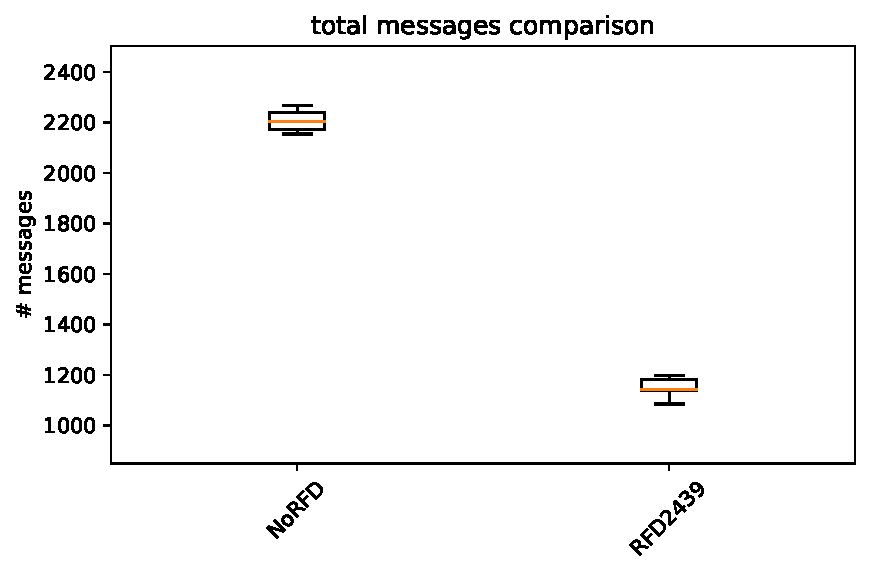
\includegraphics[width=\textwidth]{images/RFD/clique/clique_rfd_comparison_2439_messages_boxplot.pdf}
         \caption{clique topology, MRAI=30s, 10 runs, Messages comparison}
         \label{fig:RFD_2439_clique_MRAI30_messages}
     \end{subfigure}
     \hfill
     \begin{subfigure}[b]{0.49\textwidth}
         \centering
         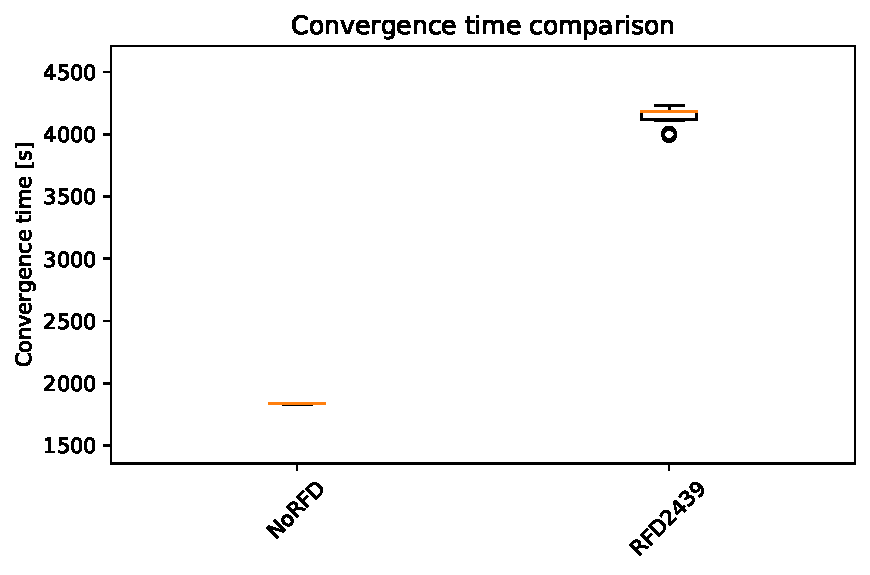
\includegraphics[width=\textwidth]{images/RFD/clique/clique_rfd_comparison_2439_time_boxplot.pdf}
         \caption{clique topology, MRAI=30s, 10 runs, Convergence time}
         \label{fig:RFD_2439_clique_MRAI30_convTime}
     \end{subfigure}
     \hfill
     \begin{subfigure}[b]{0.49\textwidth}
         \centering
         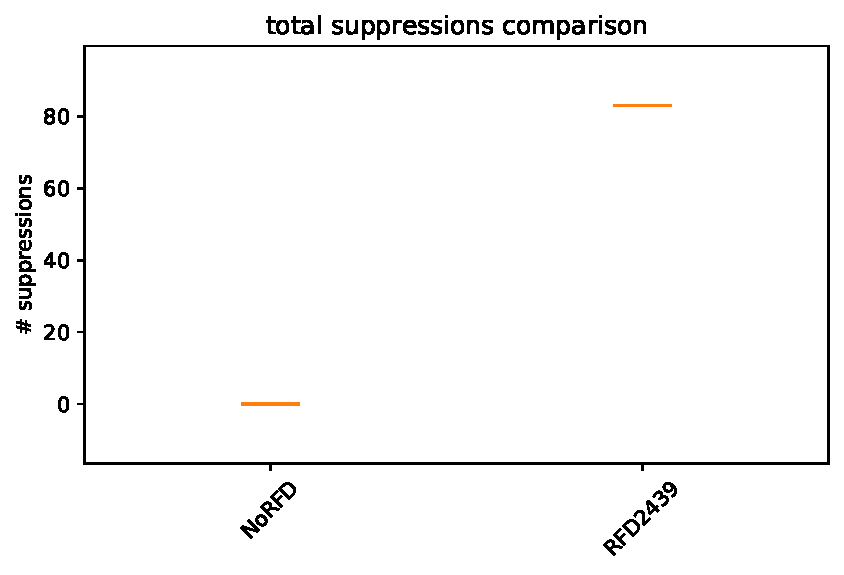
\includegraphics[width=\textwidth]{images/RFD/clique/clique_rfd_comparison_2439_suppressions_boxplot.pdf}
         \caption{clique topology, MRAI=30s, 10 runs, Number of suppressions}
         \label{fig:RFD_2439_clique_MRAI30_suppressions}
     \end{subfigure}
        \caption{Clique topology, MRAI=30s, 10 runs, comparison of the network performances}
        \label{fig:RFD_2439_MRAI30}
\end{figure}

In \Cref{fig:RFD_2439_MRAI30} is possible to see a comparison between the use
of the standard \ac{RFD} and the completely deactivation of it.
The technique \textit{NoRFD} refers to experiments executed without the
\ac{RFD} mechanisms.
This comparison goal is to show the positive effects of this technique but also
the side effects of it.
In \Cref{fig:RFD_2439_clique_MRAI30_messages} is possible to see the advantages
of \ac{RFD} while the counter effects are presented in \Cref{fig:RFD_2439_clique_MRAI30_convTime}.
The number of messages transmitted is half of the \textit{NoRFD} technique but
the cost is a more than double convergence time.
In \Cref{fig:RFD_2439_clique_MRAI30_suppressions} is possible to see the total
number of suppression executed on the entire network.
The \ac{RFD} mechanisms keep track of a different figure of merit for each neighbour,
because of that is possible that a node activate multiple suppression.
The total number of suppression activated by this environment is constant around
\num{82}.

In our case, the suppression on nodes \num{0} and \num{5} play an important role
for the network performances.
The first one for the spreading in the whole network, the second one for the
transmission of information to node $x$.

For this reason, we can look more deeply on what happened to the figure of merit
of node $x$ and five in \Cref{fig:clique_nodex_30,fig:clique_node5_30}.
The blue points represent that the route has not been suppressed yet.
Red points represent that the figure of merit has overpassed the suppression
thresholds and the route has been blocked.

\begin{figure}[h]
     \centering
     \begin{subfigure}[b]{0.476\textwidth}
         \centering
         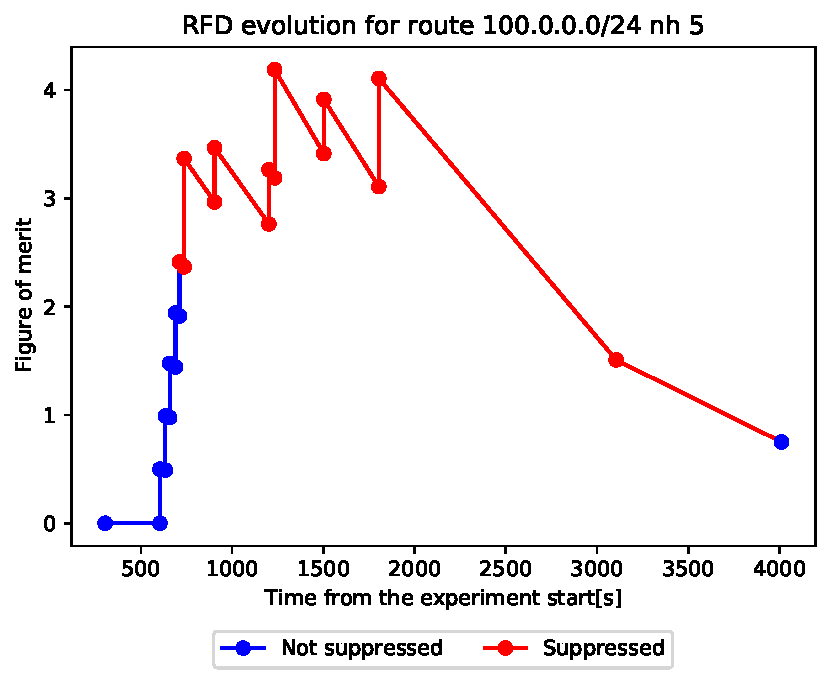
\includegraphics[width=\textwidth]{images/RFD/clique/FigureOfMerit/mrai7_RFD_x_rfd_R1.pdf}
         \caption{Node $x$ figure of merit evolution}
         \label{fig:clique_nodex_30}
     \end{subfigure}
     \hfill
     \begin{subfigure}[b]{0.494\textwidth}
         \centering
         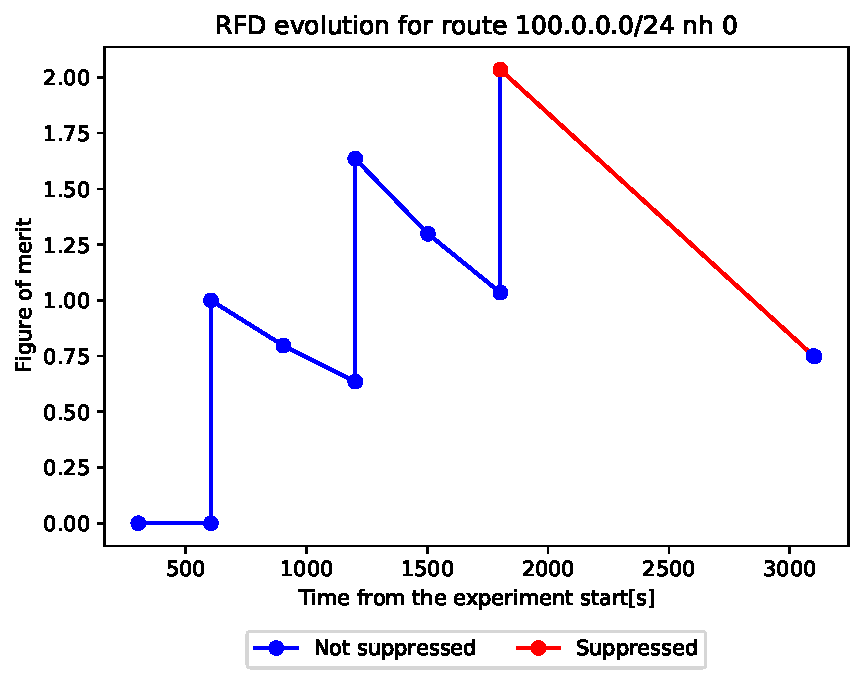
\includegraphics[width=\textwidth]{images/RFD/clique/FigureOfMerit/mrai7_RFD_5_rfd_R4.pdf}
         \caption{Node $5$ figure of merit evolution}
         \label{fig:clique_node5_30}
     \end{subfigure}
        \caption{Clique topology, MRAI=30s, figure of merit evolution
		of node \num{5} and node $x$}
        \label{fig:RFD_2439_figure_of_merit}
\end{figure}

In \Cref{fig:RFD_2439_figure_of_merit} is possible to see the two different
evolution, one of node \num{5} and the other from $x$.
Node \num{5} is the only servicer of $x$ for this reason every time it changes
its best path to reach the destination it sends an \ac{ADV} to $x$.
But, all this changes are interpreted as flaps by the \ac{RFD} filter of $x$,
for this reason the figure of merit grows very quickly.
It is sufficient a single case of \textit{Path Exploration} to provoke the
suppression of the route in $x$.
In \Cref{fig:clique_node5_30} is possible to see the evolution of the best path
of node \num{5}, the path that comes directly from \num{0}.
It takes more time for \num{5} to suppress this route, only the last flap
makes the figure of merit reach the suppression threshold.
In the same instant, around \SI{1800}{\second} also the route of $x$ gets the
last flap from \num{5} after that there is only one more point of variation
around \SI{3000}{\second}.
This last point correspond to the instant where the best route becomes available
again for \num{5}, at this point node $x$ receive the last \ac{ADV}.
But $x$ will need another \SI{1000}{\second} to makes the route available again.

We can see from this two figure of merit evolution how one depends on the other.
The evolution of $x$ strictly depend on the one from \num{5}.
And also the network performances are highly affected by that, mostly the convergence
time, because further nodes from the source will take more time to converge making
the route available again.

\section{RFC 2439 VS RFC 7196}
\label{sec:rfd_2439_Vs_7196}

%\begin{itemize}
%		\item Present RFC 7196
%		\item Experiments clique with RFC 7196 MRAI=30
%		\item Node x and 5 figure of merit
%		\item RFC 2439 VS 7196
%\end{itemize}

The difference in the two \ac{RFC} that defines \ac{RFD} \cite{rfc2439,rfc7196}
is in the parameters used.
In fact, the \ac{RFC} \num{7196} modify the figure
of merit threshold that is increased up to at least \num{6.0}, introducing
two new set of possible \ac{RFD} filters that can be used:
\begin{itemize}
	\item \textit{\textbf{Aggressive}:} Suppression threshold no less than \num{6.0};
	\item \textit{\textbf{Conservative}:} Suppression threshold no less than \num{12.0}.
\end{itemize}
Respectively \num{3} and \num{6} times the actual standard.

I have then repeated the same experiments of \Cref{sec:rfd_toy_topologies} on the same
clique graph, but with the two new \ac{RFD} strategies.
The comparison of all the strategy performances is presented in \Cref{fig:RFD_MRAI30}.

\begin{figure}[h]
     \centering
     \begin{subfigure}[b]{0.49\textwidth}
         \centering
         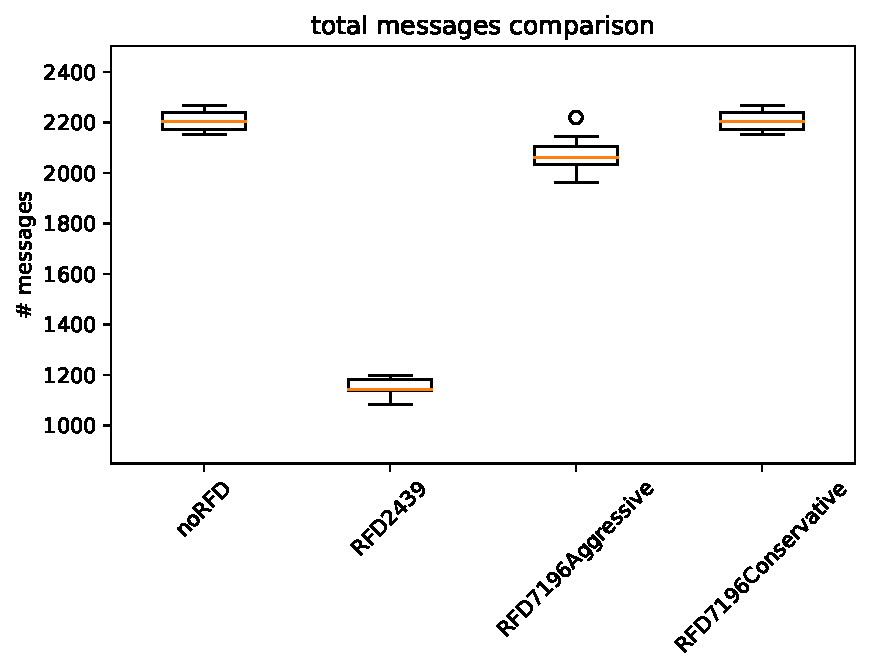
\includegraphics[width=\textwidth]{images/RFD/clique/clique_rfd_comparison_messages_boxplot.pdf}
         \caption{Messages comparison}
         \label{fig:RFD_clique_MRAI30_messages}
     \end{subfigure}
     \hfill
     \begin{subfigure}[b]{0.49\textwidth}
         \centering
         \includegraphics[width=\textwidth]{images/RFD/clique/clique_rfd_comparison_time_boxplot.pdf}
         \caption{Convergence time}
         \label{fig:RFD_clique_MRAI30_convTime}
     \end{subfigure}
     \hfill
     \begin{subfigure}[b]{0.49\textwidth}
         \centering
         \includegraphics[width=\textwidth]{images/RFD/clique/clique_rfd_comparison_suppressions_boxplot.pdf}
         \caption{Number of suppressions}
         \label{fig:RFD_clique_MRAI30_suppressions}
     \end{subfigure}
		\caption{Clique topology, MRAI equal to \SI{30}{\second}, \num{10} runs,
				comparison of the network performances with all the \ac{RFD} strategies}
        \label{fig:RFD_MRAI30}
\end{figure}

In \Cref{fig:RFD_MRAI30} is possible to see a complete comparison between all
the techniques.
Looking to \Cref{fig:RFD_clique_MRAI30_suppressions} is possible to notice that
the number of suppression can variate a lot changing the suppression threshold.
The \textit{Conservative} strategy doesn't trigger any suppression at all, while
the \textit{Aggressive} produce half the suppression of the legacy strategy.
Also, the \textit{Aggressive} strategy presents more variations in terms of
number of suppression.
Giving the fact that the conservative strategy doesn't trigger any suppression
the results in terms of performances are equal to the case without \ac{RFD}.
The consequence in the number of suppression is noticeable also in
\Cref{fig:RFD_clique_MRAI30_messages}.
The \textit{Aggressive} strategy produce on average \num{2000} messages, almost
\num{1000} more of the \ac{RFD} from the \ac{RFC} \num{2439}.

In \Cref{fig:RFD_clique_MRAI30_convTime} is possible to notice a strange behaviour.
I was expecting that having a lower number of suppression the \textit{Aggressive}
would have obtained a convergence time lower than the standard \ac{RFD}, but,
this doesn't happened.
The cause is the fact that without modifying the decay function or the reuse
threshold, the figure of merit would take a longer time to become available again.

\section{Mice VS Elephants}
\label{sec:rfd_mice_vs_elephants}

%\begin{itemize}
%		\item Present mice and elephants
%		\item present experiments environment
%\end{itemize}

From the work of R. Bush et al., \cite{pelsser2011route} we know that the majority
of the \ac{ADV} that are transmitted on the Internet are from a small set of \acp{AS}.
Those \acp{AS} with their flaps causes update storms almost continuously.
I report a figure form \cite{pelsser2011route} for simplicity in
\Cref{fig:RBushPrefixes}.
Thanks to the studies of
\ac{APNIC}\footnote{\href{https://blog.apnic.net/2020/01/15/bgp-in-2019-bgp-churn/}{APNIC BGP 2019 report}}
we also know that this behaviour is still present nowadays, the \Cref{fig:apnicPrefixes}
is taken from one of their annual reports and shows that \num{10}\% of
all the active prefixes produce more or less the \num{70}\% of the total
messages detected.

\begin{figure}[h]
     \centering
     \begin{subfigure}[b]{0.48\textwidth}
         \centering
         \includegraphics[width=\textwidth]{images/RFD/miceVSelephants/prefixVSmessagesRbush.png}
		 \caption{Prefixes and number of updates associated, figure from \cite{pelsser2011route}}
         \label{fig:RBushPrefixes}
     \end{subfigure}
     \hfill
     \begin{subfigure}[b]{0.50\textwidth}
         \centering
         \includegraphics[width=\textwidth]{images/RFD/miceVSelephants/bgp2fig5-pfx-upds-cuml.png}
         \caption{Prefixes and number of updates associated, [apnic 2019]}
         \label{fig:apnicPrefixes}
     \end{subfigure}
        \caption{Prefixes influence on updates}
        \label{fig:prefixVSmessages}
\end{figure}

We can then divide those prefixes in two sets:
\begin{itemize}
	\item \textbf{\textit{Mice}:} This set represent the majority of them,
		all the prefixes that does not generate more than \num{100} updates
		in \Cref{fig:RBushPrefixes};
	\item \textbf{\textit{Elephants}:} This set represent the remaining part
		of the prefixes, those that produces the majority of the messages.
\end{itemize}

Thanks to a annual review of \ac{BGP} by APNIC, presented at RIPE 52 \cite{huston2006bgp},
we can also have an example of those elephants prefixes.
This example is shown in \Cref{fig:ripePrefixFlaps}, it takes in consideration the
prefix \q{202.64.49.0/24} showing that in a relatively small period of time it has
produced thousands of \ac{ADV} per day.
In this case, this particular prefix has produced \num{198,370} \ac{ADV} producing
in total \num{96,330} flaps in one year.

\begin{figure}[h]
    \centering
    \includegraphics[scale=0.22]{images/RFD/miceVSelephants/ripePrefixFlap.png}
	\caption{202.64.49.0/24 flaps plot from \cite{huston2006bgp}}
    \label{fig:ripePrefixFlaps}
\end{figure}

I have then used this data to configure two new environments for the simulations.
The first one points to reproduce the \textit{Mice} behaviour, the second
one the \textit{Elephants}.

In both these environments, I have then compared the four different strategies
saw in \Cref{sec:rfd_toy_topologies,sec:rfd_2439_Vs_7196}: \textit{NoRFD},
standard \ac{RFD} from the \ac{RFC} \num{2439} and the two updated versions
from~\cite{rfc7196}.

The topology used for those experiments is an \textit{Internet like} topology
with \num{1000} nodes and \ac{MRAI} is fixed to \SI{30}{\second} for all the links.
The source of the signal has been chosen randomly on the graph.
For each experiment has been executed \num{50} runs.


\subsection{Mice}
\label{subsec:rfd_mice}

%\begin{itemize}
%		\item Present mice environment
%		\item mice experiments with MRAI=30
%\end{itemize}
The particularity of the \textit{Mice} experiments is in the signal, we have
a low number of flaps interleaved by a long timer.
I have then used a signal with \num{5} flaps, \q{AWAWAWAWAWA} with a delay
of \SI{300}{\second} (\SI{5}{\minute}) between each message.
The results are presented in \Cref{fig:1000_RFD_MRAI30_mice_bis}.
I have executed \num{50} runs for each \ac{RFD} strategy.

\begin{figure}[h]
     \centering
     \begin{subfigure}[b]{0.49\textwidth}
         \centering
         \includegraphics[width=\textwidth]{images/RFD/miceVSelephants/mice/cisco_1000MRAI30_rfd_comparison_time_boxplot.pdf}
         \caption{Convergence time respect to the RFD strategy}
         \label{fig:1000_RFD_MRAI30_mice_time_bis}
     \end{subfigure}
     \hfill
     \begin{subfigure}[b]{0.49\textwidth}
         \centering
         \includegraphics[width=\textwidth]{images/RFD/miceVSelephants/mice/cisco_1000MRAI30_rfd_comparison_messages_boxplot.pdf}
         \caption{Number of messages respect to the RFD strategy}
         \label{fig:1000_RFD_MRAI30_mice_messages_bis}
     \end{subfigure}
     \begin{subfigure}[b]{0.49\textwidth}
         \centering
         \includegraphics[width=\textwidth]{images/RFD/miceVSelephants/mice/cisco_1000MRAI30_rfd_comparison_suppressions_boxplot.pdf}
         \caption{Number of suppressions respect to the RFD strategy}
         \label{fig:1000_RFD_MRAI30_mice_suppressions_bis}
     \end{subfigure}
		\caption{Internet like topology 1000 nodes, MRAI=30s, random destination,
		5 flaps \q{AWAWAWAWAWA}, \SI{300}{\second} message delay, Network performances,
		\num{50} runs per strategy.}
        \label{fig:1000_RFD_MRAI30_mice_bis}
\end{figure}

From \Cref{fig:1000_RFD_MRAI30_mice_suppressions_bis} we can see that there is a
big difference in the number of suppression.
The standard strategy produces on average almost \num{1500} suppressions and the effects
of those suppressions can be seen in \Cref{fig:1000_RFD_MRAI30_mice_time_bis,fig:1000_RFD_MRAI30_mice_messages_bis}.
On average, it presents a convergence time higher than \SI{6000}{\second}
but with a number of total messages transmitted around \num{16000} with a very
low variance.
A different case is presented by the \textit{Conservative} strategy from \ac{RFC}
7196 \cite{rfc7196}.
The threshold in this last case is so permissive that we have a really small
number of suppression.
For this reason, the number of messages transmitted, on average, is similar to
the \textit{NoRFD} case, around \num{50000}.
While, the convergence time is around \SI{6500}{\second}, like the standard \ac{RFD}
strategy.
This proves that few suppression can heavily influence the network performances,
in particular the convergence time.
Also because the recover from a suppression with a higher threshold would require
more time.

In the middle there is the \textit{Aggressive} strategy, we can see from the
suppression boxplot that it produces a smaller number of suppression in respect
of the legacy strategy with a smaller variance.
Also, the convergence time respect this trend, in fact, the average time is
below \SI{6000}{\second}.
While The number of messages transmitted is more than double in respect
of the strategy described by the \ac{RFC} \num{2439}.

We can then conclude that a small number of suppression can affect the
performances, like the few suppressions in the \textit{Conservative} strategy
for the convergence time.
Also, the few missing suppression in the \textit{Aggressive} strategy will
enormously impact the number of messages transmitted.

Is also possible to study which are the nodes that produce the suppression and how
far are them from the signal source.
We can see the results of this study, for each suppression technique in \Cref{fig:1000_RFD_centVSsup}.

\begin{figure}[h]
     \centering
     \begin{subfigure}[b]{0.49\textwidth}
         \centering
         \includegraphics[width=\textwidth]{images/RFD/miceVSelephants/mice/cisco_1000_RFD_nodeConvergence_centVSsup_trend.pdf}
         \caption{RFD 2439 Strategy}
         \label{fig:1000_2439RFD_centVSsup}
     \end{subfigure}
     \hfill
     \begin{subfigure}[b]{0.49\textwidth}
         \centering
         \includegraphics[width=\textwidth]{images/RFD/miceVSelephants/mice/cisco_1000_RFD_7196_aggressive_nodeConvergence_centVSsup_trend.pdf}
         \caption{RFD 7196 Aggressive Strategy}
         \label{fig:1000_7196RFDA_centVSsup}
     \end{subfigure}
     \hfill
     \begin{subfigure}[b]{0.49\textwidth}
         \centering
         \includegraphics[width=\textwidth]{images/RFD/miceVSelephants/mice/cisco_1000_RFD_7196_conservative_nodeConvergence_centVSsup_trend.pdf}
         \caption{RFD 7196 Conservative Strategy}
         \label{fig:1000_7196RFDC_centVSsup}
     \end{subfigure}
		\caption{Internet like topology \num{1000} nodes, \ac{MRAI} = \SI{30}{\second},
		random destination, \num{5} flaps, \SI{300}{\second} between messages,
		Suppression trend VS avg hop distance from the source}
        \label{fig:1000_RFD_centVSsup}
\end{figure}

For the plots in \Cref{fig:1000_RFD_centVSsup} the $x$ axis represent the distance
from the source node in terms of hops and all the nodes are grouped by this
distance.
The blue line represents the average centrality of the groups, for each node of the
graph I calculated the centrality using the \ac{DPC} metric then grouped them
by the distance and calculated the average value.
As expected the central nodes have a higher centrality and are a few hops
of distance from the source node.
The centrality trend is equal for each plot in \Cref{fig:1000_RFD_centVSsup}
because the graph and the source node are the same for each experiment.

The red line represents the average number of suppressions per group.
As we can see with the standard strategy, \Cref{fig:1000_2439RFD_centVSsup},
on average, the route has been blocked \num{1} time by the nearest nodes and then,
this value increase reaching the center clique up to \num{3.5} times and then
slowly decreases in the following groups.
In the farthest group, we will still see on average \num{1} suppression.

The \textit{Aggressive} strategy, \Cref{fig:1000_7196RFDA_centVSsup} present
a similar behaviour, the nearest nodes don't block the route, while the central
nodes start blocking it with a maximum average of \num{1.6} times.
After those central nodes, the farthest nodes, that have a low centrality, will
block it on average \num{1} time, like the legacy strategy.

The \textit{Conservative} strategy, presented in \Cref{fig:1000_7196RFDC_centVSsup},
has a different trend.
We can see that the central nodes do not block the route, while only the farthest
ones block it a few times, with an average value of \num{0.2} times.
This can give us some hints, a very high threshold can promote the path
exploration problem that will cause multiple update storms in farthest nodes.

From those experiments we can see that having a higher threshold could help
to spread the knowledge near the source of the flaps, but once the
\textit{Path exploration} problem takes over, the nodes are going to suppress
the destination.
This is a good behaviour because it circumscribes an area in which the
information can spread instead of blocking it almost everywhere.
Those few suppression can highly impact in general the average convergence rate
of the network.
Is important to consider that a higher threshold means also a higher time to
make the destination available again, maybe a new decay function should be considered.


\subsection{Elephants}
\label{subsec:rfd_elephants}

%\begin{itemize}
%		\item Present elephants environment
%		\item elephants experiments with MRAI=30
%\end{itemize}

The elephants prefixes, as I mentioned in \Cref{sec:rfd_mice_vs_elephants},
are the ones that produce the majority of the \ac{ADV}.
And we also know, thanks to \cite{huston2006bgp}, that is possible to see over
thousands of messages per day.
For this reason, the \textit{elephants} environment signal is composed of \num{100}
flaps, with a delay between the messages of \SI{3}{\second}.
All the other properties of the environment are unchanged.
The results are presented in \Cref{fig:1000_RFD_MRAI_30_elephant,fig:1000_RFD_cent_VS_sup_elephants}.

\begin{figure}[h]
     \centering
     \begin{subfigure}[b]{0.49\textwidth}
         \centering
         \includegraphics[width=\textwidth]{images/RFD/miceVSelephants/elephants/cisco_1000MRAI30_rfd_comparison_time_boxplot.pdf}
         \caption{Convergence time respect to the RFD strategy}
         \label{fig:1000_RFD_MRAI_30_time_elephant}
     \end{subfigure}
     \hfill
     \begin{subfigure}[b]{0.49\textwidth}
         \centering
         \includegraphics[width=\textwidth]{images/RFD/miceVSelephants/elephants/cisco_1000MRAI30_rfd_comparison_messages_boxplot.pdf}
         \caption{Number of messages respect to the RFD strategy}
         \label{fig:1000_RFD_MRAI_30_messages_elephant}
     \end{subfigure}
     \begin{subfigure}[b]{0.49\textwidth}
         \centering
         \includegraphics[width=\textwidth]{images/RFD/miceVSelephants/elephants/cisco_1000MRAI30_rfd_comparison_suppressions_boxplot.pdf}
         \caption{Number of suppressions respect to the RFD strategy}
         \label{fig:1000_RFD_MRAI_30_suppressions_elephant}
     \end{subfigure}
		\caption{Internet like topology \num{1000} nodes, \ac{MRAI} = \SI{30}{\second},
		random destination, \num{100} flaps, \SI{3}{\second} delay between each
		message, Network performances}
        \label{fig:1000_RFD_MRAI_30_elephant}
\end{figure}

Is possible to see in \Cref{fig:1000_RFD_MRAI_30_elephant} that this time we have
a different behaviour from all the \num{3} \ac{RFD} strategies.
In \Cref{fig:1000_RFD_MRAI_30_suppressions_elephant} we can see that
the standard strategy, on average, does more than \num{1250} suppression, producing
the lowest number of messages, around \num{11000}, but the highest convergence
time with more than \SI{5000}{\second}.
All the suppression are trigger by the \textit{Path Exploration} problem that
causes \ac{ADV} storms that trigger, on the majority of the nodes, an overpass
of the critical threshold.
The two new strategies would produce on average just a few suppression in respect
of the legacy one, but the number of messages doesn't differ too much.
While there is a huge improvement on the convergence time, on average,
both the new strategy permits the network to converge in less than \SI{4000}{\second}.
All three strategy produce $1/3$ of the messages produced by the completely
absence of the \ac{RFD}.

\begin{figure}[h]
     \centering
     \begin{subfigure}[b]{0.49\textwidth}
         \centering
         \includegraphics[width=\textwidth]{images/RFD/miceVSelephants/elephants/cisco_1000_RFD_nodeConvergence_centVSsup_trend.pdf}
         \caption{RFD 2439 Strategy}
         \label{fig:1000_2439RFD_cent_VS_sup_elephants}
     \end{subfigure}
     \hfill
     \begin{subfigure}[b]{0.49\textwidth}
         \centering
         \includegraphics[width=\textwidth]{images/RFD/miceVSelephants/elephants/cisco_1000_RFD_7196_aggressive_nodeConvergence_centVSsup_trend.pdf}
         \caption{RFD 7196 Aggressive Strategy}
         \label{fig:1000_7196RFDA_cent_VS_sup_elephants}
     \end{subfigure}
     \hfill
     \begin{subfigure}[b]{0.49\textwidth}
         \centering
         \includegraphics[width=\textwidth]{images/RFD/miceVSelephants/elephants/cisco_1000_RFD_7196_conservative_nodeConvergence_centVSsup_trend.pdf}
         \caption{RFD 7196 Conservative Strategy}
         \label{fig:1000_7196RFDC_cent_VS_sup_elephants}
     \end{subfigure}
		\caption{Internet like topology \num{1000} nodes, \ac{MRAI} = \SI{30}{\second},
		random destination, \num{100} flaps, \SI{3}{\second} delay between each
		message, suppressions by distance from the source in terms of hops.
		Each point is the average of all the values produced by the nodes at the
		same distance from the source.}
        \label{fig:1000_RFD_cent_VS_sup_elephants}
\end{figure}

We can see in \Cref{fig:1000_RFD_cent_VS_sup_elephants} the comparison between
the average number of suppressions per node group of the different strategies.
In \Cref{fig:1000_7196RFDA_cent_VS_sup_elephants,fig:1000_7196RFDC_cent_VS_sup_elephants}
we can notice that both strategies, \textit{Aggressive} and \textit{Conservative},
reacts in the exact same way at the elephant environment.
The only nodes that suppress the route are the nodes that are closer to the source.
All the other nodes of the network don't experience enough messages to block
the route.

The first figure, \Cref{fig:1000_2439RFD_cent_VS_sup_elephants} shows
that, on average, every node suppress at least one time the source of the
signal.
The hypothesis behind this trend is that the number of messages that pass the
nearest nodes are enough to provoke a \textit{Path Exploration} behaviour and
with a small threshold those messages storms are enough to overcome the suppression
threshold.
With a lower threshold is sufficient a small number of \ac{ADV} storms
to trigger the \ac{RFD} suppression.

%We can then say that all the strategies catch in time the flap and avoid the
%propagation of the update storm, increasing the convergence time but protecting
%the network from thousands of messages.
With those experiments has been proven that all the strategies protect the
network from a huge load of messages.
In \Cref{fig:1000_RFD_MRAI_30_messages_elephant} we can see that the use of \ac{RFD}
reduces to $1/3$ the number of messages necessary to reach convergence.
The difference is the convergence time, more nodes experience suppression
then more time is necessary to converge because there will be more \ac{ADV} when
the figure of merit becomes lower enough to activate again the route.
For this reason there is a difference of more than \SI{1000}{\second} between
the techniques.
This experiments reinforce the hypothesis that a small number of suppressions is
more significant in respect of thousands of them.


    \chapter{Conclusion}
\label{cha:conclusion}

In this thesis, I exposed different noise problems that \ac{BGP} contains and
studied the parameters that are used to curb the problem.
I have then analyzed the results from thousands of experiments in order to
provide a solid baseline that shows how \ac{MRAI} and \ac{RFD} are related
one another.
I have also shown that, due to the \textit{Path exploration} problem, even
in small networks is really difficult to infer the causes behind a transmitted
signal.

The instruments developed during this thesis are publicly available in the
hope that other scientist could use them to study properties of \ac{BGP} that
is an extremely vast protocol.

I have then analyzed how new techniques differ from the standard or legacy one,
like in the case of \ac{RFD} where the legacy values are still present on the
internet and can have a huge impact on the convergence.
I also studied the impact that can have, in terms of performances, \ac{MRAI} on \ac{RFD},
how after a certain threshold the gain obtained from the lower number of
suppression is ininfluent in terms of convergence time and messages transmitted.

This thesis creates the basis for studies on the correlation of \ac{BGP} parameters
and would also be a warning for those studies that point to improve only
one aspect of \ac{BGP}.
Remember to always look from a different perspective because what looks like an
improvement, on the one hand, could bring the overall performance of the
network to collapse.

%\begin{itemize}
%    \item Wrap up
%    \item Path exploration explosion of the FSM
%    \item MRAI convergence dependency
%    \item RFD and MRAI co-dependency
%\end{itemize}

\section{Future Works}
\label{sec:future_works}

The development of the platform to increment the number of features is one of
the major points in the future works, but during the experiments we have also
made some assumptions/restrictions to the environment.
Those restrictions could be relaxed to study more heterogeneous environments.

\subsubsection{Policies}

One of the first assumption is that every node accept everything comes from its
neighbours and redistribute it.
This is not always true, \acp{AS} on the internet can have any sort of policy,
checking any possible attribute of the message received.
A possible future work could be to study the bibliography behind those policies
in order to be able to implement them and study again the performances of
the network with those restrictions.

\subsubsection{Multiple destinations and path aggregation}

During the experiments I never introduced more than one destination subjected to a
signal, even if the \ac{DES} permits to have multiple of them.
Obviously more destinations could produce more messages and more \ac{ADV}
storms, but a possible interesting point could be to see the reactions of the nodes
with the path aggregation activated and how it can impact the performances.

    
  \endgroup


  % bibliografia in formato bibtex
  %
  % aggiunta del capitolo nell'indice
  \addcontentsline{toc}{chapter}{References}
  % stile con ordinamento alfabetico in funzione degli autori
  \bibliographystyle{IEEEtran}
  \bibliography{references}

  \titleformat{\chapter}
      {\normalfont\Huge\bfseries}{Appendix \thechapter}{1em}{}
  % sezione Allegati - opzionale
  \appendix
  \chapter{Appendix}
\label{cha:appendx}

\begin{figure}[h]
     \centering
     \begin{subfigure}[b]{0.45\textwidth}
         \centering
         \includegraphics[width=\textwidth]{images/internet_like/1000/signals/AWAW/constant/internet_like-constant_AWAW_mrai_evolution.pdf}
		 \caption{Network perforcances, \textit{fixed} \ac{MRAI} strategy}
         \label{fig:internet_like_1000_fixed_AWAW}
     \end{subfigure}
     \hfill
     \begin{subfigure}[b]{0.45\textwidth}
         \centering
         \includegraphics[width=\textwidth]{images/internet_like/1000/signals/AWAW/dpc/internet_like-DPC_AWAW_mrai_evolution.pdf}
		 \caption{Network perforcances, \ac{DPC} \ac{MRAI} strategy}
         \label{fig:internet_like_1000_dpc_AWAW}
     \end{subfigure}
	 \caption{Network perfomances comparison with different \ac{MRAI} strategies,
		Graph internet like with \num{1000} nodes, signal \q{AWAW}}
        \label{fig:internt_like_1000_evolution_AWAW}
\end{figure}

\begin{figure}[h]
     \centering
     \begin{subfigure}[b]{0.45\textwidth}
         \centering
         \includegraphics[width=\textwidth]{images/internet_like/1000/signals/AWAWA/constant/internet_like-constant_AWAWA_mrai_evolution.pdf}
		 \caption{Network perforcances, \textit{fixed} \ac{MRAI} strategy}
         \label{fig:internet_like_1000_fixed_AWAWA}
     \end{subfigure}
     \hfill
     \begin{subfigure}[b]{0.45\textwidth}
         \centering
         \includegraphics[width=\textwidth]{images/internet_like/1000/signals/AWAWA/dpc/internet_like-DPC_AWAWA_mrai_evolution.pdf}
		 \caption{Network perforcances, \ac{DPC} \ac{MRAI} strategy}
         \label{fig:internet_like_1000_dpc_AWAWA}
     \end{subfigure}
	 \caption{Network perfomances comparison with different \ac{MRAI} strategies,
		Graph internet like with \num{1000} nodes, signal \q{AWAWA}}
        \label{fig:internt_like_1000_evolution_AWAWA}
\end{figure}

\begin{figure}[h]
     \centering
     \begin{subfigure}[b]{0.45\textwidth}
         \centering
         \includegraphics[width=\textwidth]{images/internet_like/1000/comparison/comparison_AWA_messages_boxplot.pdf}
		 \caption{Network perforcances, messages necessary to reach convergence
			with different \ac{MRAI} strategies}
         \label{fig:boxplot_internet_like_1000_messages_AWA}
     \end{subfigure}
     \hfill
     \begin{subfigure}[b]{0.45\textwidth}
         \centering
         \includegraphics[width=\textwidth]{images/internet_like/1000/comparison/comparison_AWA_time_boxplot.pdf}
		 \caption{Network perforcances, time required to reach convergence
			with different \ac{MRAI} strategies}
         \label{fig:boxplot_internet_like_1000_time_AWA}
     \end{subfigure}
	 \caption{Network perfomances comparison with different \ac{MRAI} strategies,
		Graph internet like with \num{1000} nodes, \ac{MRAI} value 
		\SI{30}{\second}, number of runs for each strategy \num{100}, signal \q{AWA}}
        \label{fig:boxplot_internet_like_1000_AWA}
\end{figure}

\begin{figure}[h]
     \centering
     \begin{subfigure}[b]{0.45\textwidth}
         \centering
         \includegraphics[width=\textwidth]{images/internet_like/1000/comparison/comparison_AWAW_messages_boxplot.pdf}
		 \caption{Network perforcances, messages necessary to reach convergence
			with different \ac{MRAI} strategies}
         \label{fig:boxplot_internet_like_1000_messages_AWAW}
     \end{subfigure}
     \hfill
     \begin{subfigure}[b]{0.45\textwidth}
         \centering
         \includegraphics[width=\textwidth]{images/internet_like/1000/comparison/comparison_AWAW_time_boxplot.pdf}
		 \caption{Network perforcances, time required to reach convergence
			with different \ac{MRAI} strategies}
         \label{fig:boxplot_internet_like_1000_time_AWAW}
     \end{subfigure}
	 \caption{Network perfomances comparison with different \ac{MRAI} strategies,
		Graph internet like with \num{1000} nodes, \ac{MRAI} value 
		\SI{30}{\second}, number of runs for each strategy \num{100}, signal \q{AWAW}}
        \label{fig:boxplot_internet_like_1000_AWAW}
\end{figure}

\begin{figure}[h]
     \centering
     \begin{subfigure}[b]{0.45\textwidth}
         \centering
         \includegraphics[width=\textwidth]{images/internet_like/1000/comparison/comparison_AWAWA_messages_boxplot.pdf}
		 \caption{Network perforcances, messages necessary to reach convergence
			with different \ac{MRAI} strategies}
         \label{fig:boxplot_internet_like_1000_messages_AWAWA}
     \end{subfigure}
     \hfill
     \begin{subfigure}[b]{0.45\textwidth}
         \centering
         \includegraphics[width=\textwidth]{images/internet_like/1000/comparison/comparison_AWAWA_time_boxplot.pdf}
		 \caption{Network perforcances, time required to reach convergence
			with different \ac{MRAI} strategies}
         \label{fig:boxplot_internet_like_1000_time_AWAWA}
     \end{subfigure}
	 \caption{Network perfomances comparison with different \ac{MRAI} strategies,
		Graph internet like with \num{1000} nodes, \ac{MRAI} value 
		\SI{30}{\second}, number of runs for each strategy \num{100}, signal \q{AWAWA}}
        \label{fig:boxplot_internet_like_1000_AWAWA}
\end{figure}

\begin{figure}[h]
    \centering
    \includegraphics[width=\textwidth]{images/RFD/clique/cisco_clique10_RFD_comparison_constant_all.pdf}
	\caption{Comparison of the \textit{clique} topology with RFD 2439 and the with 
		RFD 7196 strategies}
    \label{fig:clique_RFD2439VSRFD7196}
\end{figure}

\begin{figure}[h]
     \centering
     \begin{subfigure}[b]{0.3\textwidth}
         \centering
         \includegraphics[width=\textwidth]{images/RFD/clique/clique_rfd_comparison_messages_boxplot.pdf}
         \caption{clique topology, MRAI=30s, 10 runs, Messages comparison}
         \label{fig:RFD_MRAI30_messages}
     \end{subfigure}
     \hfill
     \begin{subfigure}[b]{0.3\textwidth}
         \centering
         \includegraphics[width=\textwidth]{images/RFD/clique/clique_rfd_comparison_time_boxplot.pdf}
         \caption{clique topology, MRAI=30s, 10 runs, Convergence time}
         \label{fig:RFD_MRAI30_convTime}
     \end{subfigure}
     \hfill
     \begin{subfigure}[b]{0.3\textwidth}
         \centering
         \includegraphics[width=\textwidth]{images/RFD/clique/clique_rfd_comparison_suppressions_boxplot.pdf}
         \caption{clique topology, MRAI=30s, 10 runs, Number of suppressions}
         \label{fig:RFD_MRAI30_suppressions}
     \end{subfigure}
        \caption{Clique topology, MRAI=30s, 10 runs, comparison of the network performances}
        \label{fig:RFD_MRAI30}
\end{figure}
\clearpage

\begin{figure}[H]
     \centering
     \begin{subfigure}[b]{0.325\textwidth}
         \centering
         \includegraphics[width=\textwidth]{images/RFD/miceVSelephants/MultiMRAI/0/mice/cisco_1000MRAI0_rfd_comparison_time_boxplot.pdf}
         \caption{Convergence time respect to the RFD strategy, MRAI=0s}
         \label{fig:1000_RFD_MRAI0_time_mice}
     \end{subfigure}
     \hfill
     \begin{subfigure}[b]{0.325\textwidth}
         \centering
         \includegraphics[width=\textwidth]{images/RFD/miceVSelephants/MultiMRAI/0/mice/cisco_1000MRAI0_rfd_comparison_messages_boxplot.pdf}
         \caption{Number of messages respect to the RFD strategy, MRAI=0s}
         \label{fig:1000_RFD_MRAI0_messages_mice}
     \end{subfigure}
     \hfill
     \begin{subfigure}[b]{0.325\textwidth}
         \centering
         \includegraphics[width=\textwidth]{images/RFD/miceVSelephants/MultiMRAI/0/mice/cisco_1000MRAI0_rfd_comparison_suppressions_boxplot.pdf}
         \caption{Number of suppressions respect to the RFD strategy, MRAI=0s}
         \label{fig:1000_RFD_MRAI0_suppressions_mice}
     \end{subfigure}
     \vfill
     \begin{subfigure}[b]{0.325\textwidth}
         \centering
         \includegraphics[width=\textwidth]{images/RFD/miceVSelephants/MultiMRAI/15/mice/cisco_1000MRAI15_rfd_comparison_time_boxplot.pdf}
         \caption{Convergence time respect to the RFD strategy, MRAI=15s}
         \label{fig:1000_RFD_MRAI15_time_mice}
     \end{subfigure}
     \hfill
     \begin{subfigure}[b]{0.325\textwidth}
         \centering
         \includegraphics[width=\textwidth]{images/RFD/miceVSelephants/MultiMRAI/15/mice/cisco_1000MRAI15_rfd_comparison_messages_boxplot.pdf}
         \caption{Number of messages respect to the RFD strategy, MRAI=15s}
         \label{fig:1000_RFD_MRAI15_messages_mice}
     \end{subfigure}
     \hfill
     \begin{subfigure}[b]{0.325\textwidth}
         \centering
         \includegraphics[width=\textwidth]{images/RFD/miceVSelephants/MultiMRAI/15/mice/cisco_1000MRAI15_rfd_comparison_suppressions_boxplot.pdf}
         \caption{Number of suppressions respect to the RFD strategy, MRAI=15s}
         \label{fig:1000_RFD_MRAI15_suppressions_mice}
     \end{subfigure}
     \vfill
     \begin{subfigure}[b]{0.325\textwidth}
         \centering
         \includegraphics[width=\textwidth]{images/RFD/miceVSelephants/MultiMRAI/30/mice/cisco_1000MRAI30_rfd_comparison_time_boxplot.pdf}
         \caption{Convergence time respect to the RFD strategy, MRAI=30s}
         \label{fig:1000_RFD_MRAI30_time_mice}
     \end{subfigure}
     \hfill
     \begin{subfigure}[b]{0.325\textwidth}
         \centering
         \includegraphics[width=\textwidth]{images/RFD/miceVSelephants/MultiMRAI/30/mice/cisco_1000MRAI30_rfd_comparison_messages_boxplot.pdf}
         \caption{Number of messages respect to the RFD strategy, MRAI=30s}
         \label{fig:1000_RFD_MRAI30_messages_mice}
     \end{subfigure}
     \hfill
     \begin{subfigure}[b]{0.325\textwidth}
         \centering
         \includegraphics[width=\textwidth]{images/RFD/miceVSelephants/MultiMRAI/30/mice/cisco_1000MRAI30_rfd_comparison_suppressions_boxplot.pdf}
         \caption{Number of suppressions respect to the RFD strategy, MRAI=30s}
         \label{fig:1000_RFD_MRAI30_suppressions_mice}
     \end{subfigure}
     \vfill
     \begin{subfigure}[b]{0.325\textwidth}
         \centering
         \includegraphics[width=\textwidth]{images/RFD/miceVSelephants/MultiMRAI/45/mice/cisco_1000MRAI45_rfd_comparison_time_boxplot.pdf}
         \caption{Convergence time respect to the RFD strategy, MRAI=45s}
         \label{fig:1000_RFD_MRAI45_time_mice}
     \end{subfigure}
     \hfill
     \begin{subfigure}[b]{0.325\textwidth}
         \centering
         \includegraphics[width=\textwidth]{images/RFD/miceVSelephants/MultiMRAI/45/mice/cisco_1000MRAI45_rfd_comparison_messages_boxplot.pdf}
         \caption{Number of messages respect to the RFD strategy, MRAI=30s}
         \label{fig:1000_RFD_MRAI45_messages_mice}
     \end{subfigure}
     \hfill
     \begin{subfigure}[b]{0.325\textwidth}
         \centering
         \includegraphics[width=\textwidth]{images/RFD/miceVSelephants/MultiMRAI/45/mice/cisco_1000MRAI45_rfd_comparison_suppressions_boxplot.pdf}
         \caption{Number of suppressions respect to the RFD strategy, MRAI=45s}
         \label{fig:1000_RFD_MRAI45_suppressions_mice}
     \end{subfigure}
     \vfill
     \begin{subfigure}[b]{0.325\textwidth}
         \centering
         \includegraphics[width=\textwidth]{images/RFD/miceVSelephants/MultiMRAI/60/mice/cisco_1000MRAI60_rfd_comparison_time_boxplot.pdf}
         \caption{Convergence time respect to the RFD strategy, MRAI=60s}
         \label{fig:1000_RFD_MRAI60_time_mice}
     \end{subfigure}
     \hfill
     \begin{subfigure}[b]{0.325\textwidth}
         \centering
         \includegraphics[width=\textwidth]{images/RFD/miceVSelephants/MultiMRAI/60/mice/cisco_1000MRAI60_rfd_comparison_messages_boxplot.pdf}
         \caption{Number of messages respect to the RFD strategy, MRAI=60s}
         \label{fig:1000_RFD_MRAI60_messages_mice}
     \end{subfigure}
     \hfill
     \begin{subfigure}[b]{0.325\textwidth}
         \centering
         \includegraphics[width=\textwidth]{images/RFD/miceVSelephants/MultiMRAI/60/mice/cisco_1000MRAI60_rfd_comparison_suppressions_boxplot.pdf}
         \caption{Number of suppressions respect to the RFD strategy, MRAI=60s}
         \label{fig:1000_RFD_MRAI60_suppressions_mice}
     \end{subfigure}
        \caption{Internet like topology 1000 nodes, random destination, 5 flaps, 300s delay, Network performances}
        \label{fig:1000_RFD_MRAI30_mice}
\end{figure}

\begin{figure}[H]
     \centering
     \begin{subfigure}[b]{0.325\textwidth}
         \centering
         \includegraphics[width=\textwidth]{images/RFD/miceVSelephants/MultiMRAI/0/mice/cisco_1000_RFD_nodeConvergence_centVSsup_trend.pdf}
         \caption{RFD 2439 Strategy, \\MRAI=0s}
         \label{fig:1000_2439RFD_centVSsup_mices_MRAI0}
     \end{subfigure}
     \hfill
     \begin{subfigure}[b]{0.325\textwidth}
         \centering
         \includegraphics[width=\textwidth]{images/RFD/miceVSelephants/MultiMRAI/0/mice/cisco_1000_RFD_7196_aggressive_nodeConvergence_centVSsup_trend.pdf}
         \caption{RFD 7196 Aggressive Strategy, MRAI=0s}
         \label{fig:1000_7196RFDA_centVSsup_mices_MRAI0}
     \end{subfigure}
     \hfill
     \begin{subfigure}[b]{0.325\textwidth}
         \centering
         \includegraphics[width=\textwidth]{images/RFD/miceVSelephants/MultiMRAI/0/mice/cisco_1000_RFD_7196_conservative_nodeConvergence_centVSsup_trend.pdf}
         \caption{RFD 7196 Conservative Strategy, MRAI=0s}
         \label{fig:1000_7196RFDC_centVSsup_mices_MRAI0}
     \end{subfigure}
     \vfill
     \begin{subfigure}[b]{0.325\textwidth}
         \centering
         \includegraphics[width=\textwidth]{images/RFD/miceVSelephants/MultiMRAI/15/mice/cisco_1000_RFD_nodeConvergence_centVSsup_trend.pdf}
         \caption{RFD 2439 Strategy, \\MRAI=15s}
         \label{fig:1000_2439RFD_centVSsup_mices_MRAI15}
     \end{subfigure}
     \hfill
     \begin{subfigure}[b]{0.325\textwidth}
         \centering
         \includegraphics[width=\textwidth]{images/RFD/miceVSelephants/MultiMRAI/15/mice/cisco_1000_RFD_7196_aggressive_nodeConvergence_centVSsup_trend.pdf}
         \caption{RFD 7196 Aggressive Strategy, MRAI=15s}
         \label{fig:1000_7196RFDA_centVSsup_mices_MRAI15}
     \end{subfigure}
     \hfill
     \begin{subfigure}[b]{0.325\textwidth}
         \centering
         \includegraphics[width=\textwidth]{images/RFD/miceVSelephants/MultiMRAI/15/mice/cisco_1000_RFD_7196_conservative_nodeConvergence_centVSsup_trend.pdf}
         \caption{RFD 7196 Conservative Strategy, MRAI=15s}
         \label{fig:1000_7196RFDC_centVSsup_mices_MRAI15}
     \end{subfigure}
     \vfill
     \begin{subfigure}[b]{0.325\textwidth}
         \centering
         \includegraphics[width=\textwidth]{images/RFD/miceVSelephants/MultiMRAI/30/mice/cisco_1000_RFD_nodeConvergence_centVSsup_trend.pdf}
         \caption{RFD 2439 Strategy, \\MRAI=30s}
         \label{fig:1000_2439RFD_centVSsup_mices_MRAI30}
     \end{subfigure}
     \hfill
     \begin{subfigure}[b]{0.325\textwidth}
         \centering
         \includegraphics[width=\textwidth]{images/RFD/miceVSelephants/MultiMRAI/30/mice/cisco_1000_RFD_7196_aggressive_nodeConvergence_centVSsup_trend.pdf}
         \caption{RFD 7196 Aggressive Strategy, MRAI=30s}
         \label{fig:1000_7196RFDA_centVSsup_mices_MRAI30}
     \end{subfigure}
     \hfill
     \begin{subfigure}[b]{0.325\textwidth}
         \centering
         \includegraphics[width=\textwidth]{images/RFD/miceVSelephants/MultiMRAI/30/mice/cisco_1000_RFD_7196_conservative_nodeConvergence_centVSsup_trend.pdf}
         \caption{RFD 7196 Conservative Strategy, MRAI=30s}
         \label{fig:1000_7196RFDC_centVSsup_mices_MRAI30}
     \end{subfigure}
     \vfill
     \begin{subfigure}[b]{0.325\textwidth}
         \centering
         \includegraphics[width=\textwidth]{images/RFD/miceVSelephants/MultiMRAI/45/mice/cisco_1000_RFD_nodeConvergence_centVSsup_trend.pdf}
         \caption{RFD 2439 Strategy, \\MRAI=45s}
         \label{fig:1000_2439RFD_centVSsup_mices_MRAI45}
     \end{subfigure}
     \hfill
     \begin{subfigure}[b]{0.325\textwidth}
         \centering
         \includegraphics[width=\textwidth]{images/RFD/miceVSelephants/MultiMRAI/45/mice/cisco_1000_RFD_7196_aggressive_nodeConvergence_centVSsup_trend.pdf}
         \caption{RFD 7196 Aggressive Strategy, MRAI=45s}
         \label{fig:1000_7196RFDA_centVSsup_mices_MRAI45}
     \end{subfigure}
     \hfill
     \begin{subfigure}[b]{0.325\textwidth}
         \centering
         \includegraphics[width=\textwidth]{images/RFD/miceVSelephants/MultiMRAI/45/mice/cisco_1000_RFD_7196_conservative_nodeConvergence_centVSsup_trend.pdf}
         \caption{RFD 7196 Conservative Strategy, MRAI=45s}
         \label{fig:1000_7196RFDC_centVSsup_mices_MRAI45}
     \end{subfigure}
     \vfill
     \begin{subfigure}[b]{0.325\textwidth}
         \centering
         \includegraphics[width=\textwidth]{images/RFD/miceVSelephants/MultiMRAI/60/mice/cisco_1000_RFD_nodeConvergence_centVSsup_trend.pdf}
         \caption{RFD 2439 Strategy, \\MRAI=60s}
         \label{fig:1000_2439RFD_centVSsup_mices_MRAI60}
     \end{subfigure}
     \hfill
     \begin{subfigure}[b]{0.325\textwidth}
         \centering
         \includegraphics[width=\textwidth]{images/RFD/miceVSelephants/MultiMRAI/60/mice/cisco_1000_RFD_7196_aggressive_nodeConvergence_centVSsup_trend.pdf}
         \caption{RFD 7196 Aggressive Strategy, MRAI=60s}
         \label{fig:1000_7196RFDA_centVSsup_mices_MRAI60}
     \end{subfigure}
     \hfill
     \begin{subfigure}[b]{0.325\textwidth}
         \centering
         \includegraphics[width=\textwidth]{images/RFD/miceVSelephants/MultiMRAI/60/mice/cisco_1000_RFD_7196_conservative_nodeConvergence_centVSsup_trend.pdf}
         \caption{RFD 7196 Conservative Strategy, MRAI=60s}
         \label{fig:1000_7196RFDC_centVSsup_mices_MRAI60}
     \end{subfigure}
        \caption{Internet like topology 1000 nodes, random destination, 5 flaps, 300s delay, Suppression trend VS avg hop centrality}
        \label{fig:1000_RFD_centVSsup_mices}
\end{figure}

\begin{figure}[H]
     \centering
     \begin{subfigure}[b]{0.325\textwidth}
         \centering
         \includegraphics[width=\textwidth]{images/RFD/miceVSelephants/MultiMRAI/0/elephants/cisco_1000MRAI0_rfd_comparison_time_boxplot.pdf}
         \caption{Convergence time respect to the RFD strategy, MRAI=0s}
         \label{fig:1000_RFD_MRAI0_time_elephant}
     \end{subfigure}
     \hfill
     \begin{subfigure}[b]{0.325\textwidth}
         \centering
         \includegraphics[width=\textwidth]{images/RFD/miceVSelephants/MultiMRAI/0/elephants/cisco_1000MRAI0_rfd_comparison_messages_boxplot.pdf}
         \caption{Number of messages respect to the RFD strategy, MRAI=0s}
         \label{fig:1000_RFD_MRAI0_messages_elephant}
     \end{subfigure}
     \hfill
     \begin{subfigure}[b]{0.325\textwidth}
         \centering
         \includegraphics[width=\textwidth]{images/RFD/miceVSelephants/MultiMRAI/0/elephants/cisco_1000MRAI0_rfd_comparison_suppressions_boxplot.pdf}
         \caption{Number of suppressions respect to the RFD strategy, MRAI=0s}
         \label{fig:1000_RFD_MRAI0_suppressions_elephant}
     \end{subfigure}
     \vfill
     \begin{subfigure}[b]{0.325\textwidth}
         \centering
         \includegraphics[width=\textwidth]{images/RFD/miceVSelephants/MultiMRAI/15/elephants/cisco_1000MRAI15_rfd_comparison_time_boxplot.pdf}
         \caption{Convergence time respect to the RFD strategy, MRAI=15s}
         \label{fig:1000_RFD_MRAI15_time_elephant}
     \end{subfigure}
     \hfill
     \begin{subfigure}[b]{0.325\textwidth}
         \centering
         \includegraphics[width=\textwidth]{images/RFD/miceVSelephants/MultiMRAI/15/elephants/cisco_1000MRAI15_rfd_comparison_messages_boxplot.pdf}
         \caption{Number of messages respect to the RFD strategy, MRAI=15s}
         \label{fig:1000_RFD_MRAI15_messages_elephant}
     \end{subfigure}
     \hfill
     \begin{subfigure}[b]{0.325\textwidth}
         \centering
         \includegraphics[width=\textwidth]{images/RFD/miceVSelephants/MultiMRAI/15/elephants/cisco_1000MRAI15_rfd_comparison_suppressions_boxplot.pdf}
         \caption{Number of suppressions respect to the RFD strategy, MRAI=15s}
         \label{fig:1000_RFD_MRAI15_suppressions_elephant}
     \end{subfigure}
     \vfill
     \begin{subfigure}[b]{0.325\textwidth}
         \centering
         \includegraphics[width=\textwidth]{images/RFD/miceVSelephants/MultiMRAI/30/elephants/cisco_1000MRAI30_rfd_comparison_time_boxplot.pdf}
         \caption{Convergence time respect to the RFD strategy, MRAI=30s}
         \label{fig:1000_RFD_MRAI30_time_elephant}
     \end{subfigure}
     \hfill
     \begin{subfigure}[b]{0.325\textwidth}
         \centering
         \includegraphics[width=\textwidth]{images/RFD/miceVSelephants/MultiMRAI/30/elephants/cisco_1000MRAI30_rfd_comparison_messages_boxplot.pdf}
         \caption{Number of messages respect to the RFD strategy, MRAI=30s}
         \label{fig:1000_RFD_MRAI30_messages_elephant}
     \end{subfigure}
     \hfill
     \begin{subfigure}[b]{0.325\textwidth}
         \centering
         \includegraphics[width=\textwidth]{images/RFD/miceVSelephants/MultiMRAI/30/elephants/cisco_1000MRAI30_rfd_comparison_suppressions_boxplot.pdf}
         \caption{Number of suppressions respect to the RFD strategy, MRAI=30s}
         \label{fig:1000_RFD_MRAI30_suppressions_elephant}
     \end{subfigure}
     \vfill
     \begin{subfigure}[b]{0.325\textwidth}
         \centering
         \includegraphics[width=\textwidth]{images/RFD/miceVSelephants/MultiMRAI/45/elephants/cisco_1000MRAI45_rfd_comparison_time_boxplot.pdf}
         \caption{Convergence time respect to the RFD strategy, MRAI=45s}
         \label{fig:1000_RFD_MRAI45_time_elephant}
     \end{subfigure}
     \hfill
     \begin{subfigure}[b]{0.325\textwidth}
         \centering
         \includegraphics[width=\textwidth]{images/RFD/miceVSelephants/MultiMRAI/45/elephants/cisco_1000MRAI45_rfd_comparison_messages_boxplot.pdf}
         \caption{Number of messages respect to the RFD strategy, MRAI=30s}
         \label{fig:1000_RFD_MRAI45_messages_elephant}
     \end{subfigure}
     \hfill
     \begin{subfigure}[b]{0.325\textwidth}
         \centering
         \includegraphics[width=\textwidth]{images/RFD/miceVSelephants/MultiMRAI/45/elephants/cisco_1000MRAI45_rfd_comparison_suppressions_boxplot.pdf}
         \caption{Number of suppressions respect to the RFD strategy, MRAI=45s}
         \label{fig:1000_RFD_MRAI45_suppressions_elephant}
     \end{subfigure}
     \vfill
     \begin{subfigure}[b]{0.325\textwidth}
         \centering
         \includegraphics[width=\textwidth]{images/RFD/miceVSelephants/MultiMRAI/60/elephants/cisco_1000MRAI60_rfd_comparison_time_boxplot.pdf}
         \caption{Convergence time respect to the RFD strategy, MRAI=60s}
         \label{fig:1000_RFD_MRAI60_time_elephant}
     \end{subfigure}
     \hfill
     \begin{subfigure}[b]{0.325\textwidth}
         \centering
         \includegraphics[width=\textwidth]{images/RFD/miceVSelephants/MultiMRAI/60/elephants/cisco_1000MRAI60_rfd_comparison_messages_boxplot.pdf}
         \caption{Number of messages respect to the RFD strategy, MRAI=60s}
         \label{fig:1000_RFD_MRAI60_messages_elephant}
     \end{subfigure}
     \hfill
     \begin{subfigure}[b]{0.325\textwidth}
         \centering
         \includegraphics[width=\textwidth]{images/RFD/miceVSelephants/MultiMRAI/60/elephants/cisco_1000MRAI60_rfd_comparison_suppressions_boxplot.pdf}
         \caption{Number of suppressions respect to the RFD strategy, MRAI=60s}
         \label{fig:1000_RFD_MRAI60_suppressions_elephant}
     \end{subfigure}
        \caption{Internet like topology 1000 nodes, random destination, 100 flaps, 3s delay, Network performances}
        \label{fig:1000_RFD_MRAI30_elephant}
\end{figure}

\begin{figure}[H]
     \centering
     \begin{subfigure}[b]{0.325\textwidth}
         \centering
         \includegraphics[width=\textwidth]{images/RFD/miceVSelephants/MultiMRAI/0/elephants/cisco_1000_RFD_nodeConvergence_centVSsup_trend.pdf}
         \caption{RFD 2439 Strategy, \\MRAI=0s}
         \label{fig:1000_2439RFD_centVSsup_elephants_MRAI0}
     \end{subfigure}
     \hfill
     \begin{subfigure}[b]{0.325\textwidth}
         \centering
         \includegraphics[width=\textwidth]{images/RFD/miceVSelephants/MultiMRAI/0/elephants/cisco_1000_RFD_7196_aggressive_nodeConvergence_centVSsup_trend.pdf}
         \caption{RFD 7196 Aggressive Strategy, MRAI=0s}
         \label{fig:1000_7196RFDA_centVSsup_elephants_MRAI0}
     \end{subfigure}
     \hfill
     \begin{subfigure}[b]{0.325\textwidth}
         \centering
         \includegraphics[width=\textwidth]{images/RFD/miceVSelephants/MultiMRAI/0/elephants/cisco_1000_RFD_7196_conservative_nodeConvergence_centVSsup_trend.pdf}
         \caption{RFD 7196 Conservative Strategy, MRAI=0s}
         \label{fig:1000_7196RFDC_centVSsup_elephants_MRAI0}
     \end{subfigure}
     \vfill
     \begin{subfigure}[b]{0.325\textwidth}
         \centering
         \includegraphics[width=\textwidth]{images/RFD/miceVSelephants/MultiMRAI/15/elephants/cisco_1000_RFD_nodeConvergence_centVSsup_trend.pdf}
         \caption{RFD 2439 Strategy, \\MRAI=15s}
         \label{fig:1000_2439RFD_centVSsup_elephants_MRAI15}
     \end{subfigure}
     \hfill
     \begin{subfigure}[b]{0.325\textwidth}
         \centering
         \includegraphics[width=\textwidth]{images/RFD/miceVSelephants/MultiMRAI/15/elephants/cisco_1000_RFD_7196_aggressive_nodeConvergence_centVSsup_trend.pdf}
         \caption{RFD 7196 Aggressive Strategy, MRAI=15s}
         \label{fig:1000_7196RFDA_centVSsup_elephants_MRAI15}
     \end{subfigure}
     \hfill
     \begin{subfigure}[b]{0.325\textwidth}
         \centering
         \includegraphics[width=\textwidth]{images/RFD/miceVSelephants/MultiMRAI/15/elephants/cisco_1000_RFD_7196_conservative_nodeConvergence_centVSsup_trend.pdf}
         \caption{RFD 7196 Conservative Strategy, MRAI=15s}
         \label{fig:1000_7196RFDC_centVSsup_elephants_MRAI15}
     \end{subfigure}
     \vfill
     \begin{subfigure}[b]{0.325\textwidth}
         \centering
         \includegraphics[width=\textwidth]{images/RFD/miceVSelephants/MultiMRAI/30/elephants/cisco_1000_RFD_nodeConvergence_centVSsup_trend.pdf}
         \caption{RFD 2439 Strategy, \\MRAI=30s}
         \label{fig:1000_2439RFD_centVSsup_elephants_MRAI30}
     \end{subfigure}
     \hfill
     \begin{subfigure}[b]{0.325\textwidth}
         \centering
         \includegraphics[width=\textwidth]{images/RFD/miceVSelephants/MultiMRAI/30/elephants/cisco_1000_RFD_7196_aggressive_nodeConvergence_centVSsup_trend.pdf}
         \caption{RFD 7196 Aggressive Strategy, MRAI=30s}
         \label{fig:1000_7196RFDA_centVSsup_elephants_MRAI30}
     \end{subfigure}
     \hfill
     \begin{subfigure}[b]{0.325\textwidth}
         \centering
         \includegraphics[width=\textwidth]{images/RFD/miceVSelephants/MultiMRAI/30/elephants/cisco_1000_RFD_7196_conservative_nodeConvergence_centVSsup_trend.pdf}
         \caption{RFD 7196 Conservative Strategy, MRAI=30s}
         \label{fig:1000_7196RFDC_centVSsup_elephants_MRAI30}
     \end{subfigure}
     \vfill
     \begin{subfigure}[b]{0.325\textwidth}
         \centering
         \includegraphics[width=\textwidth]{images/RFD/miceVSelephants/MultiMRAI/45/elephants/cisco_1000_RFD_nodeConvergence_centVSsup_trend.pdf}
         \caption{RFD 2439 Strategy, \\MRAI=45s}
         \label{fig:1000_2439RFD_centVSsup_elephants_MRAI45}
     \end{subfigure}
     \hfill
     \begin{subfigure}[b]{0.325\textwidth}
         \centering
         \includegraphics[width=\textwidth]{images/RFD/miceVSelephants/MultiMRAI/45/elephants/cisco_1000_RFD_7196_aggressive_nodeConvergence_centVSsup_trend.pdf}
         \caption{RFD 7196 Aggressive Strategy, MRAI=45s}
         \label{fig:1000_7196RFDA_centVSsup_elephants_MRAI45}
     \end{subfigure}
     \hfill
     \begin{subfigure}[b]{0.325\textwidth}
         \centering
         \includegraphics[width=\textwidth]{images/RFD/miceVSelephants/MultiMRAI/45/elephants/cisco_1000_RFD_7196_conservative_nodeConvergence_centVSsup_trend.pdf}
         \caption{RFD 7196 Conservative Strategy, MRAI=45s}
         \label{fig:1000_7196RFDC_centVSsup_elephants_MRAI45}
     \end{subfigure}
     \vfill
     \begin{subfigure}[b]{0.325\textwidth}
         \centering
         \includegraphics[width=\textwidth]{images/RFD/miceVSelephants/MultiMRAI/60/elephants/cisco_1000_RFD_nodeConvergence_centVSsup_trend.pdf}
         \caption{RFD 2439 Strategy, \\MRAI=60s}
         \label{fig:1000_2439RFD_centVSsup_elephants_MRAI60}
     \end{subfigure}
     \hfill
     \begin{subfigure}[b]{0.325\textwidth}
         \centering
         \includegraphics[width=\textwidth]{images/RFD/miceVSelephants/MultiMRAI/60/elephants/cisco_1000_RFD_7196_aggressive_nodeConvergence_centVSsup_trend.pdf}
         \caption{RFD 7196 Aggressive Strategy, MRAI=60s}
         \label{fig:1000_7196RFDA_centVSsup_elephants_MRAI60}
     \end{subfigure}
     \hfill
     \begin{subfigure}[b]{0.325\textwidth}
         \centering
         \includegraphics[width=\textwidth]{images/RFD/miceVSelephants/MultiMRAI/60/elephants/cisco_1000_RFD_7196_conservative_nodeConvergence_centVSsup_trend.pdf}
         \caption{RFD 7196 Conservative Strategy, MRAI=60s}
         \label{fig:1000_7196RFDC_centVSsup_elephants_MRAI60}
     \end{subfigure}
        \caption{Internet like topology 1000 nodes, random destination, 100 flaps, 3s delay, Suppression trend VS avg hop centrality}
        \label{fig:1000_RFD_centVSsup_elephants}
\end{figure}

  \printacronyms[name=Abbreviations]
  \addcontentsline{toc}{chapter}{Abbreviations}

\end{document}
